% \begin{figure}[H]
%   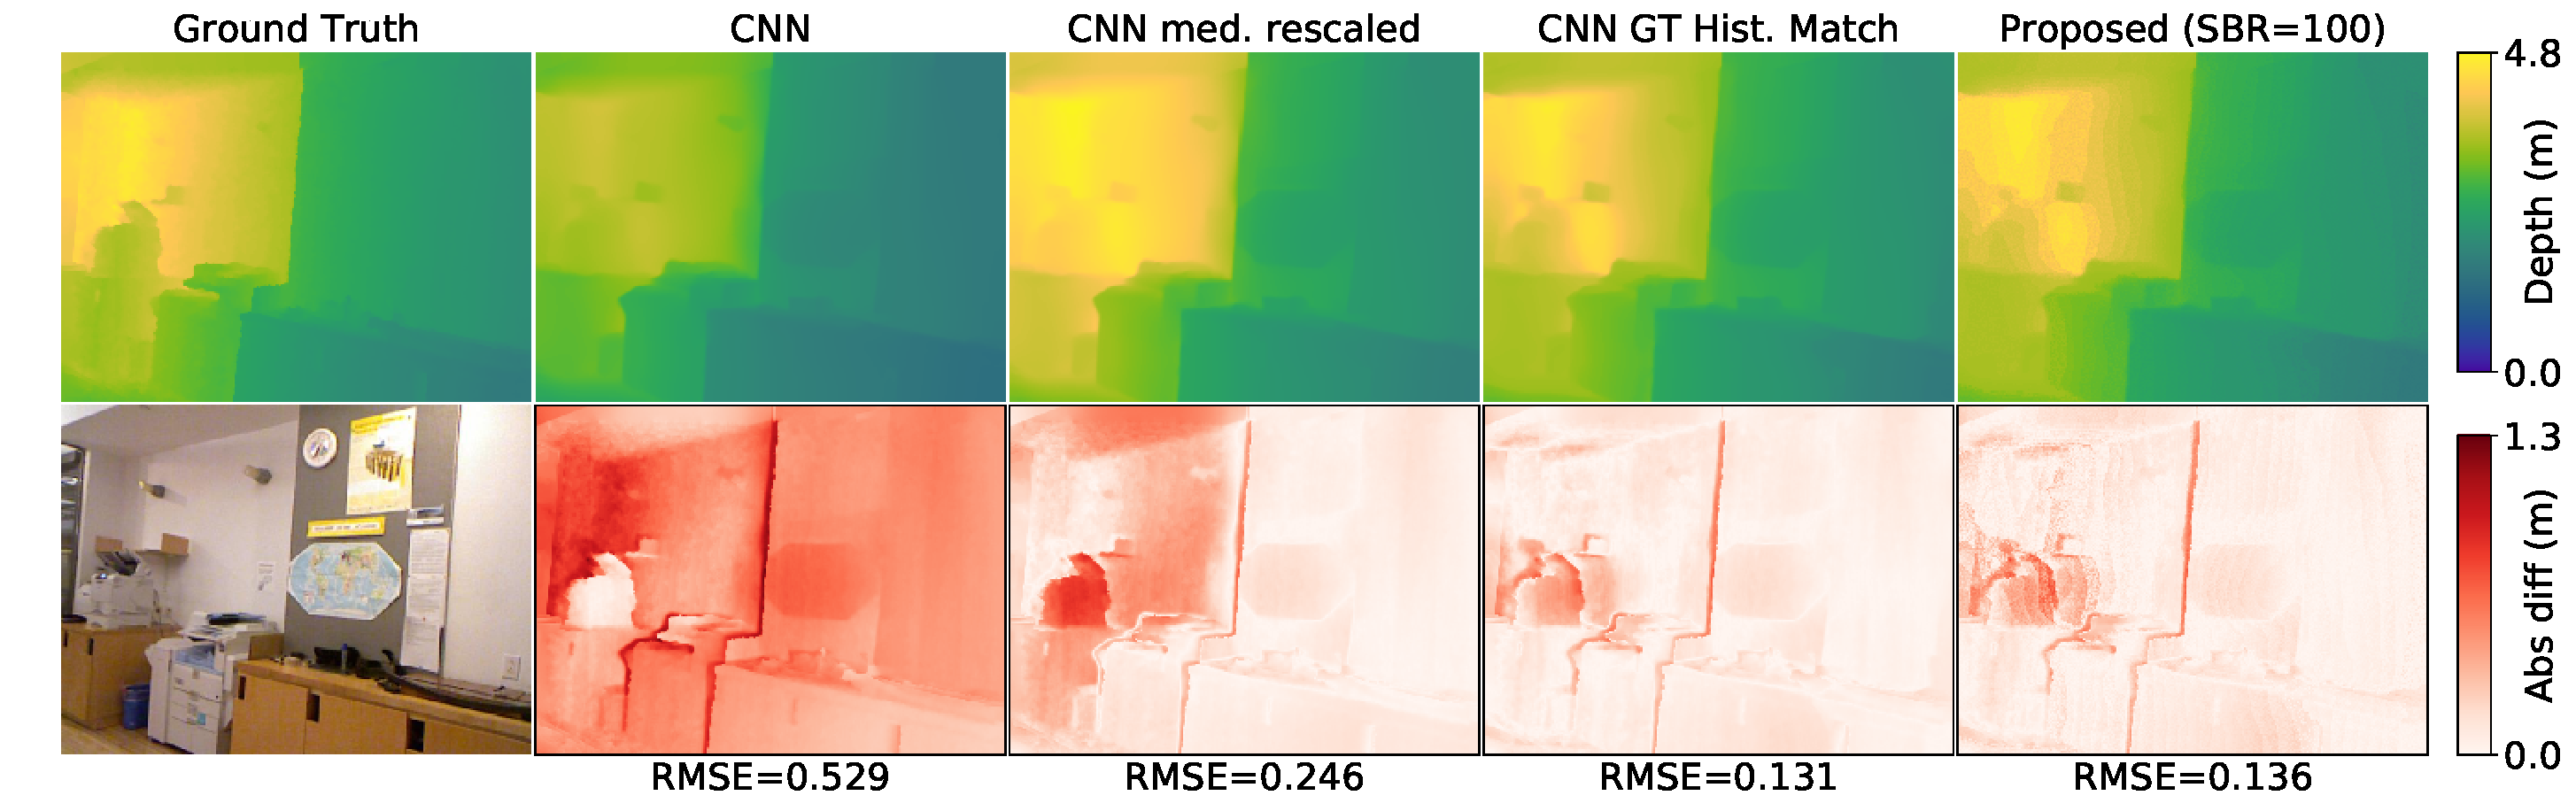
\includegraphics[width=\textwidth]{comparison/densedepth_18_comparison.pdf}
%   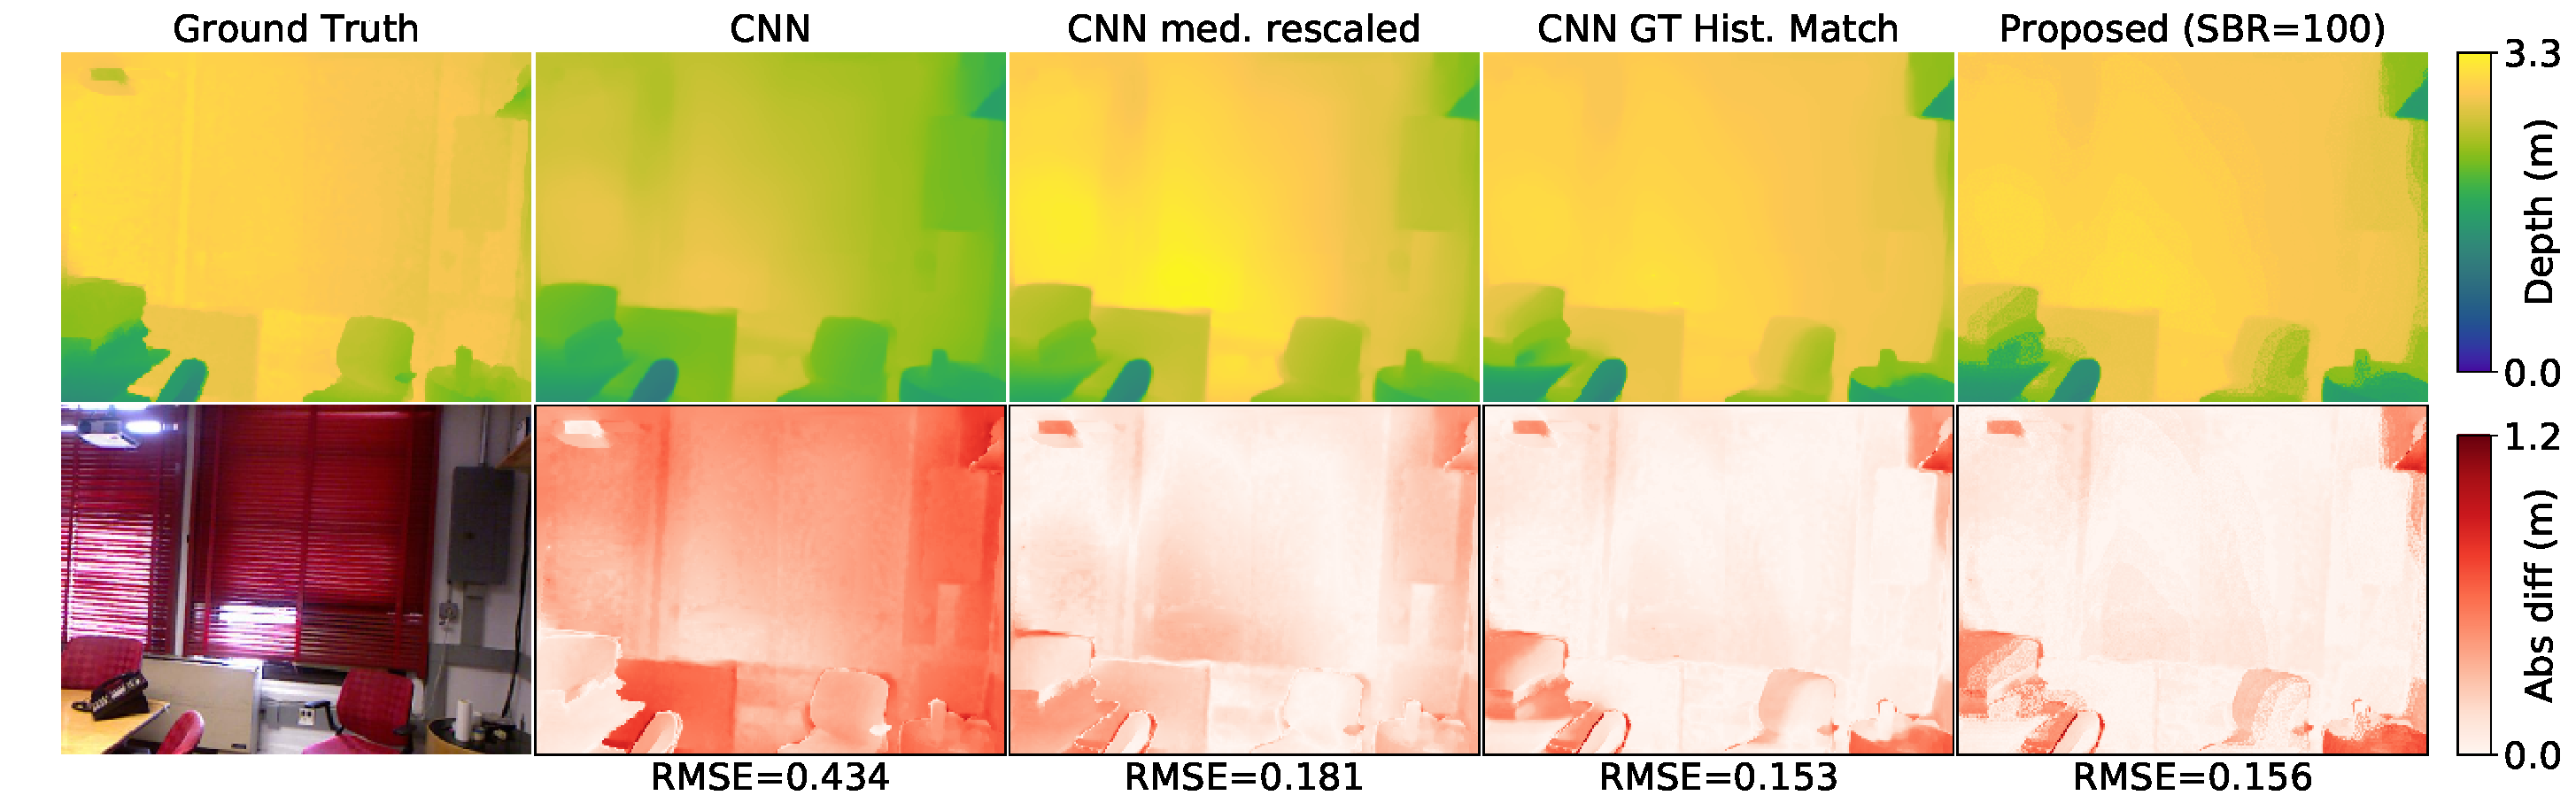
\includegraphics[width=\textwidth]{comparison/densedepth_21_comparison.pdf}
%   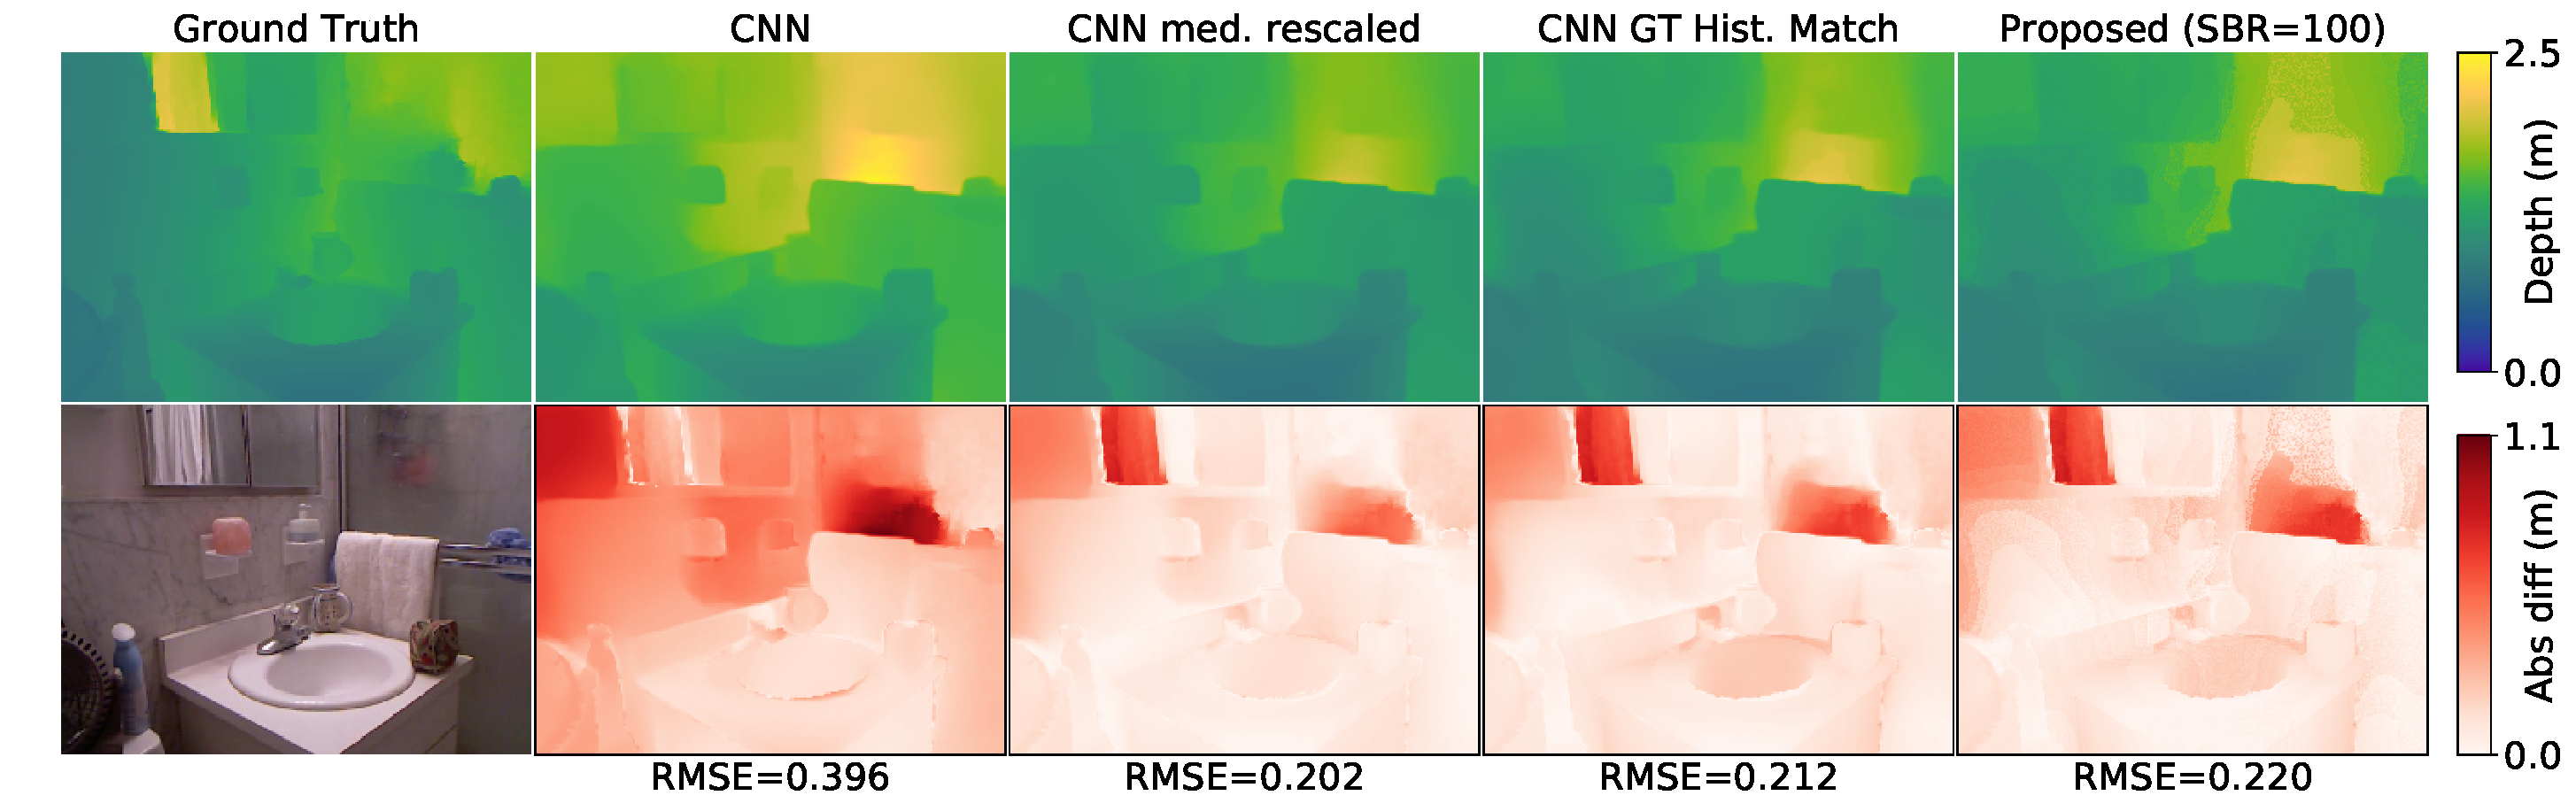
\includegraphics[width=\textwidth]{comparison/densedepth_25_comparison.pdf}
%   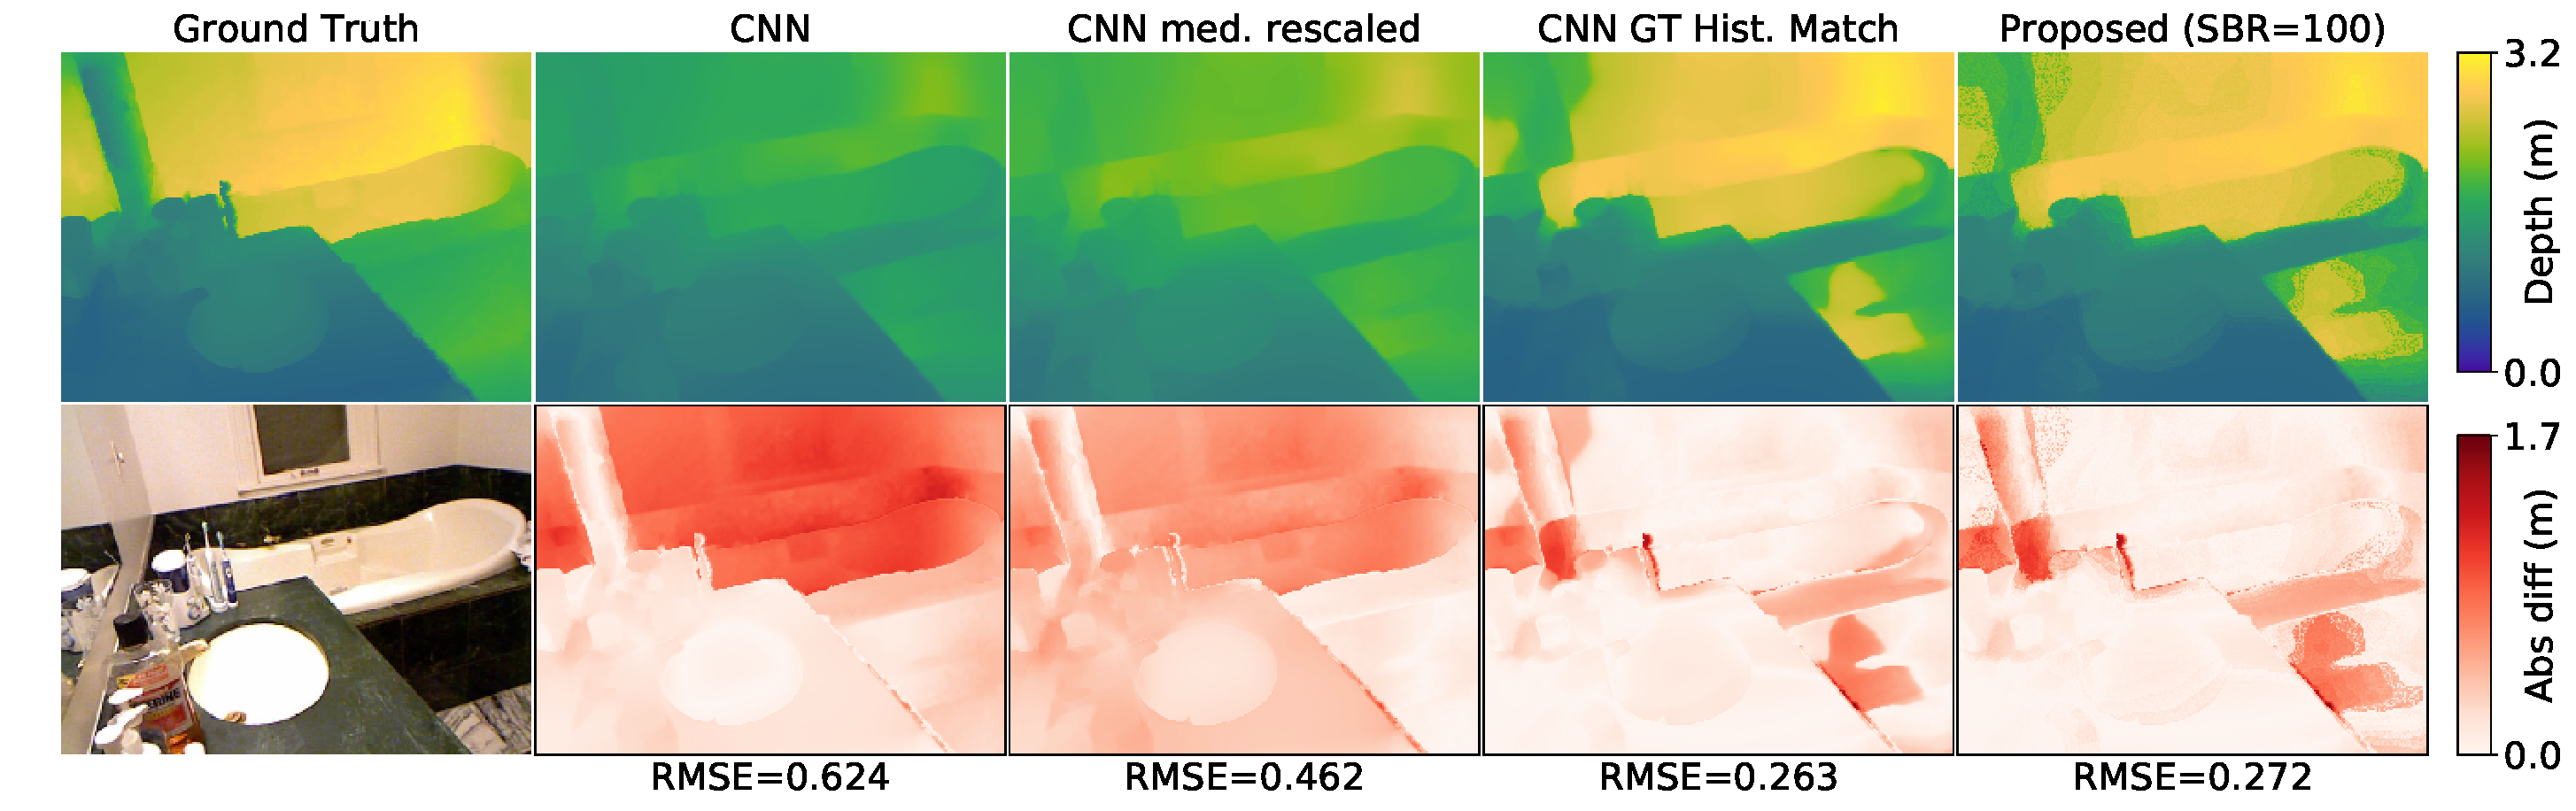
\includegraphics[width=\textwidth]{comparison/densedepth_194_comparison.pdf}
%   \caption{Results with DenseDepth as the MDE. Our method is able to scale and
%     shift the depth maps to mitigate gross errors in depth scaling.}
%   \label{fig:densedepth_1}
% \end{figure}
\begin{figure}[H]
  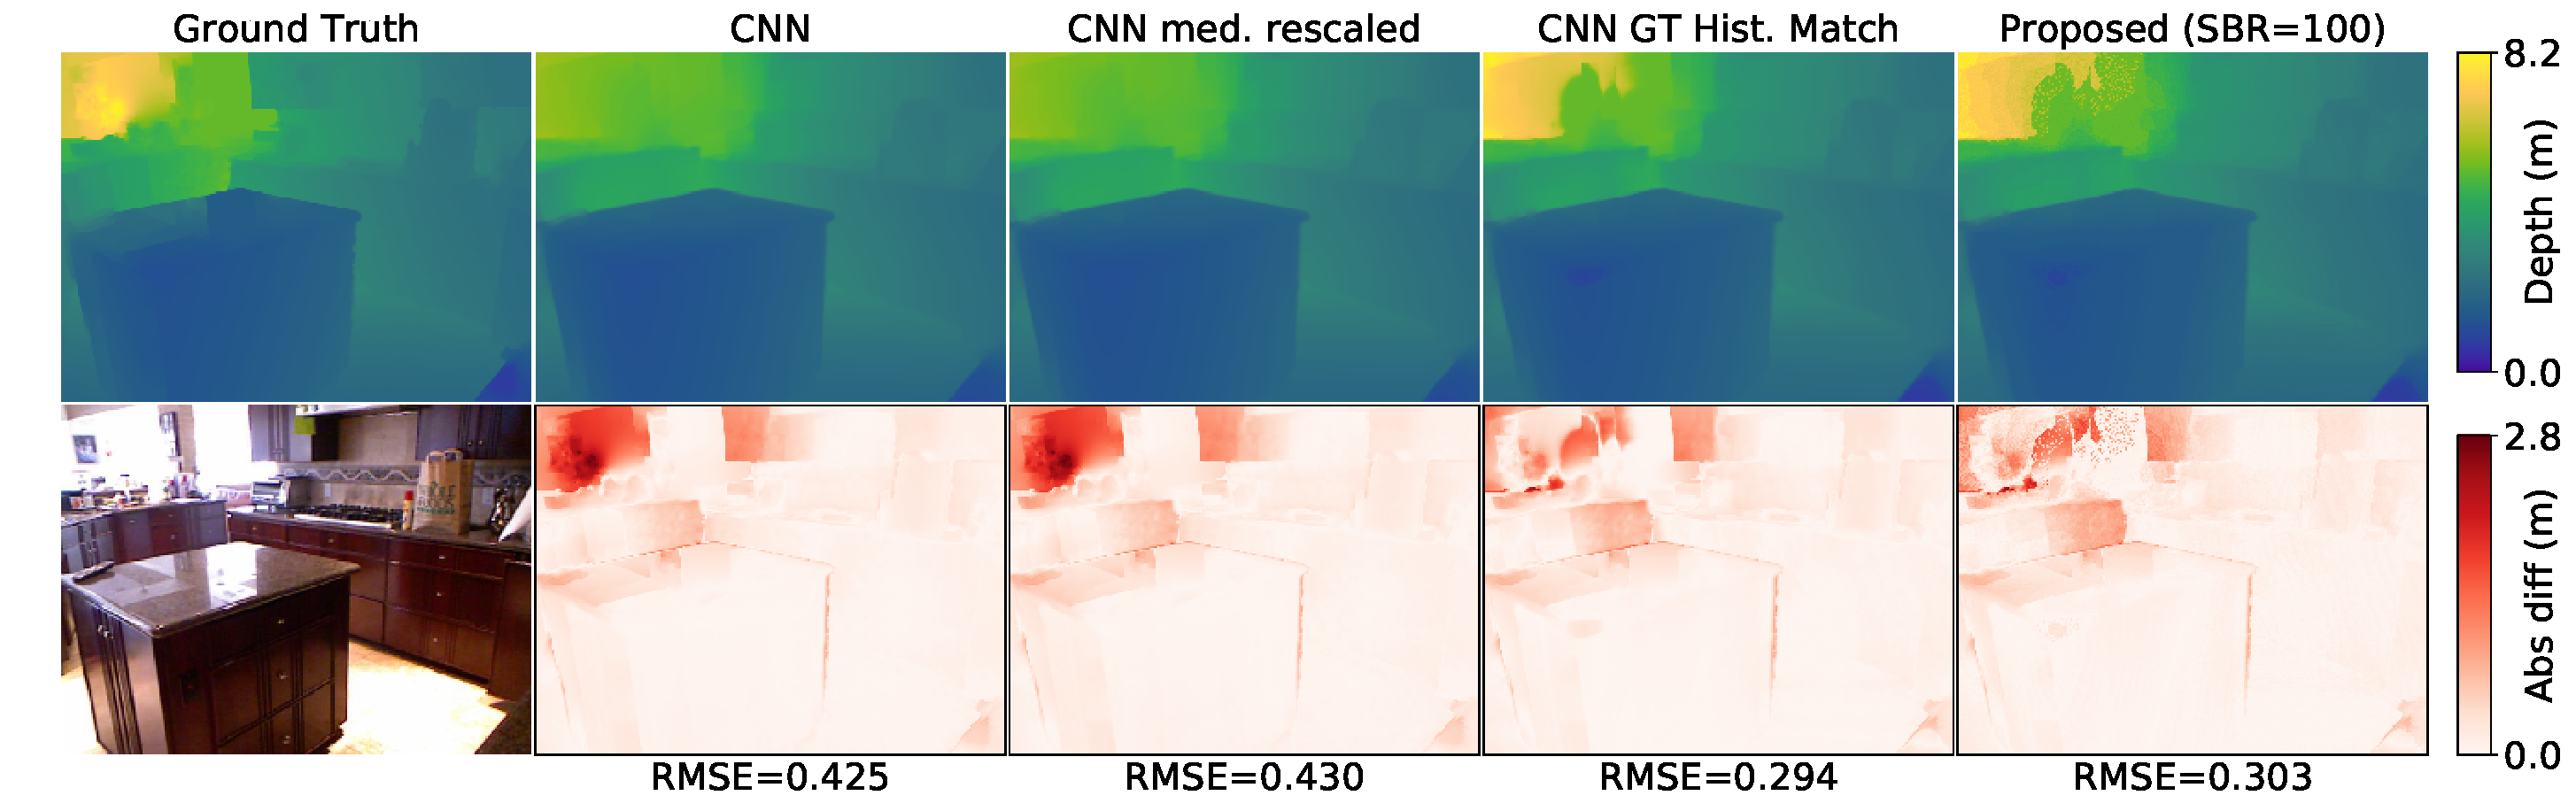
\includegraphics[width=\textwidth]{comparison/densedepth_362_comparison.pdf}
  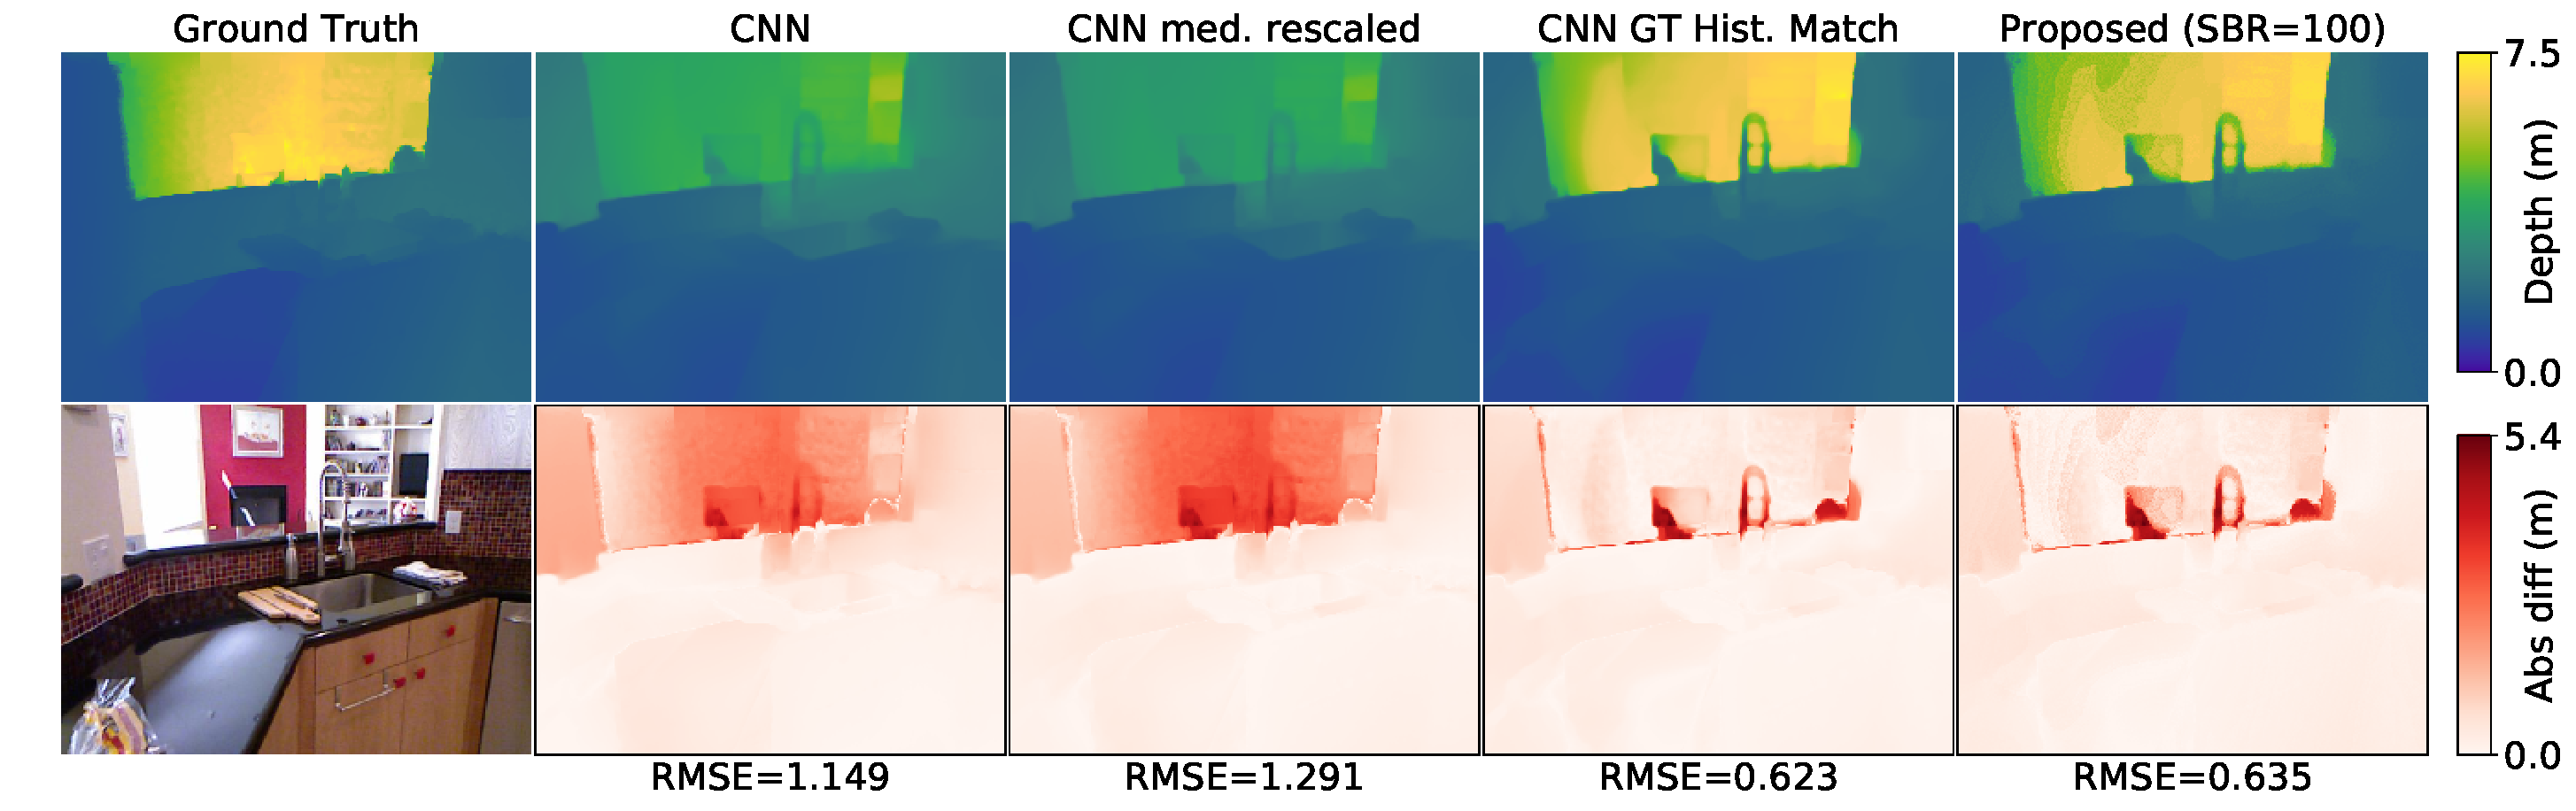
\includegraphics[width=\textwidth]{comparison/densedepth_379_comparison.pdf}
  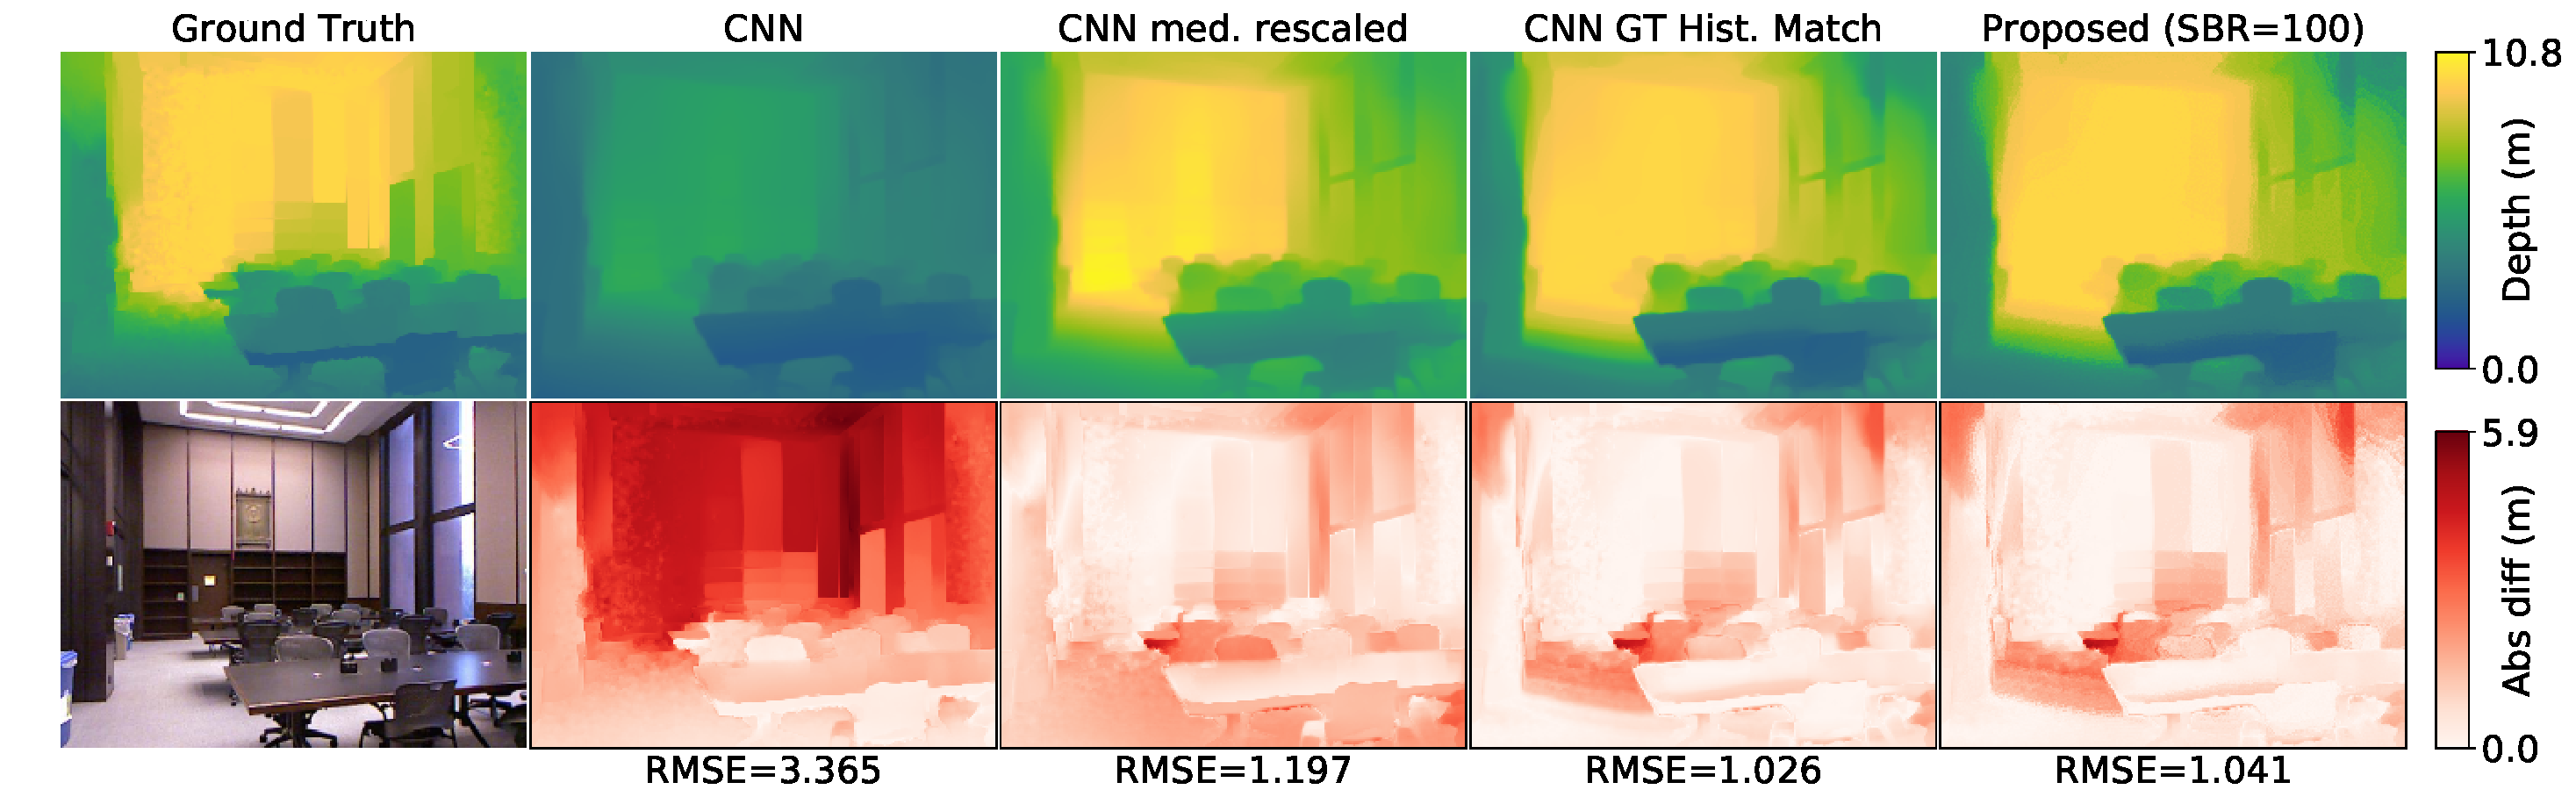
\includegraphics[width=\textwidth]{comparison/densedepth_107_comparison.pdf}
  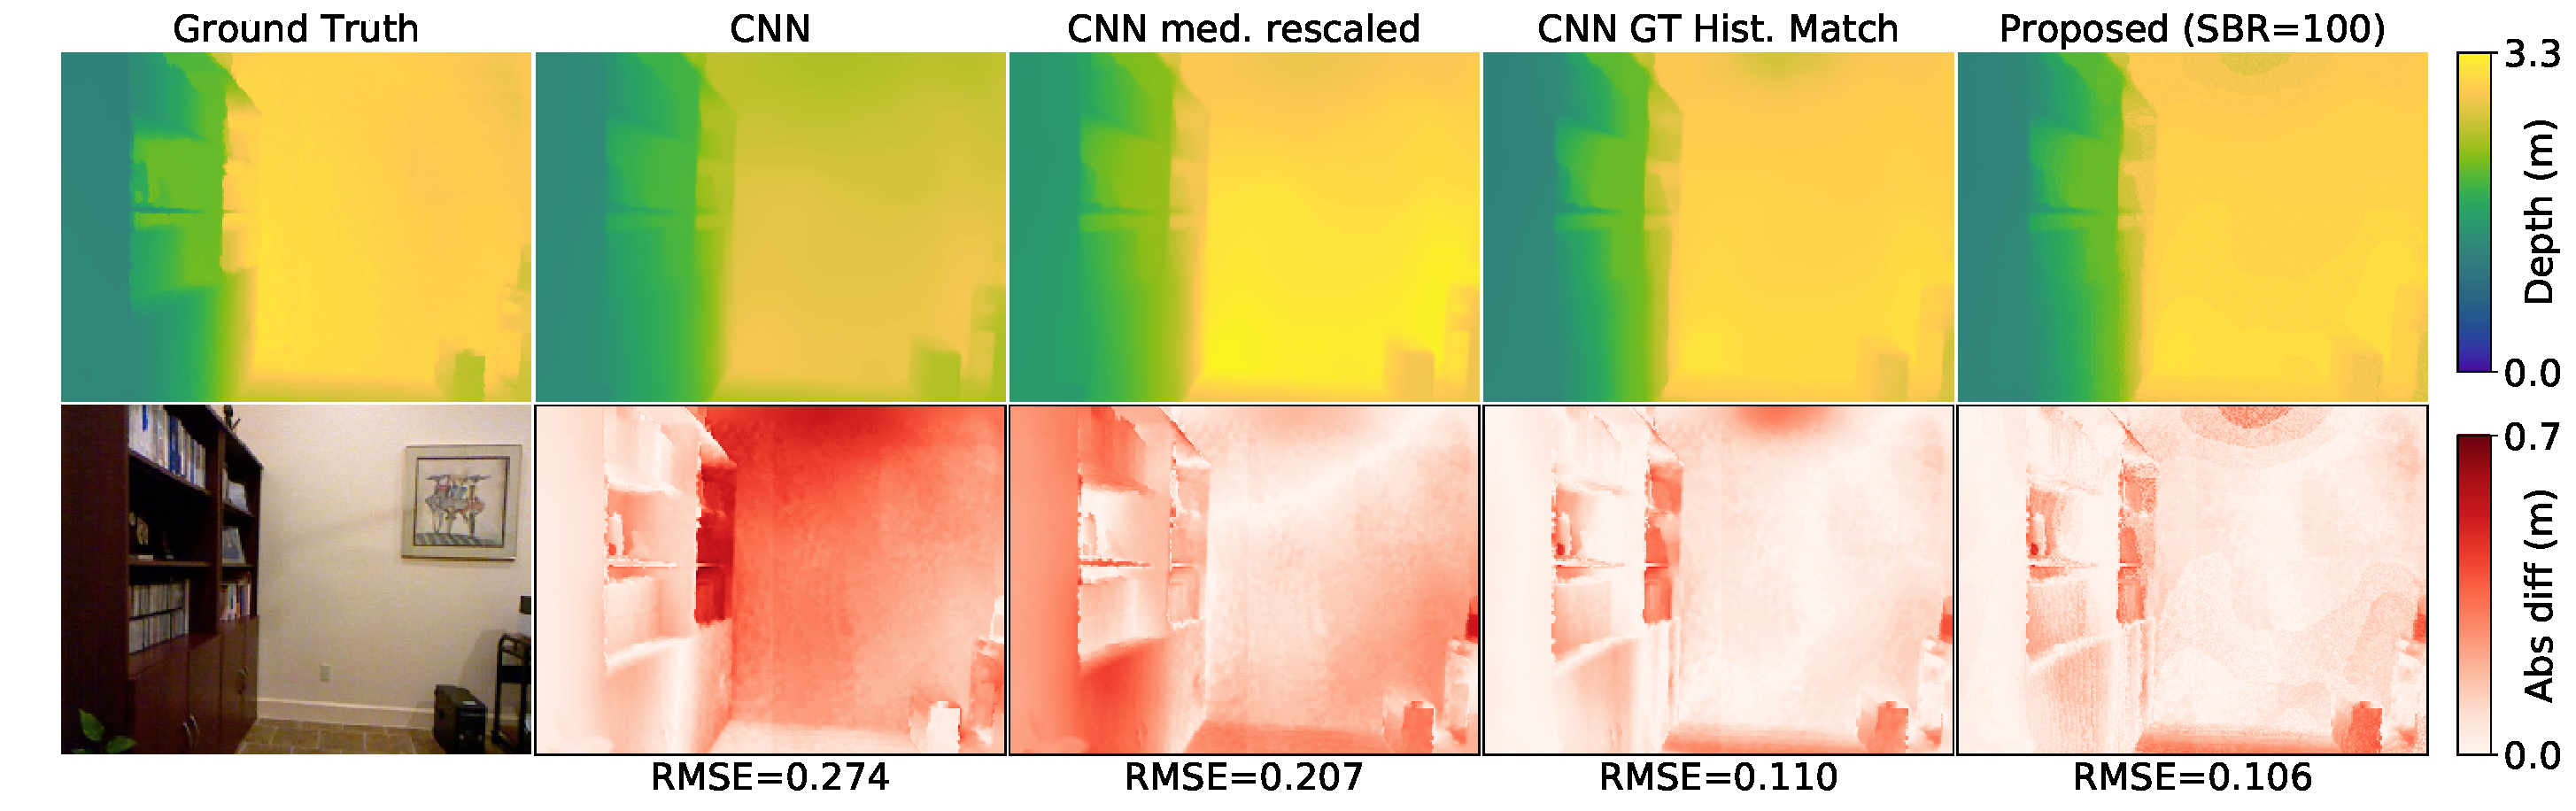
\includegraphics[width=\textwidth]{comparison/densedepth_187_comparison.pdf}
  \caption{Results with DenseDepth as the monocular depth estimator. Our method is able to scale and
    shift the depth maps to mitigate gross errors in depth scaling.}
  \label{fig:densedepth_1}
\end{figure}
\begin{figure}[H]
  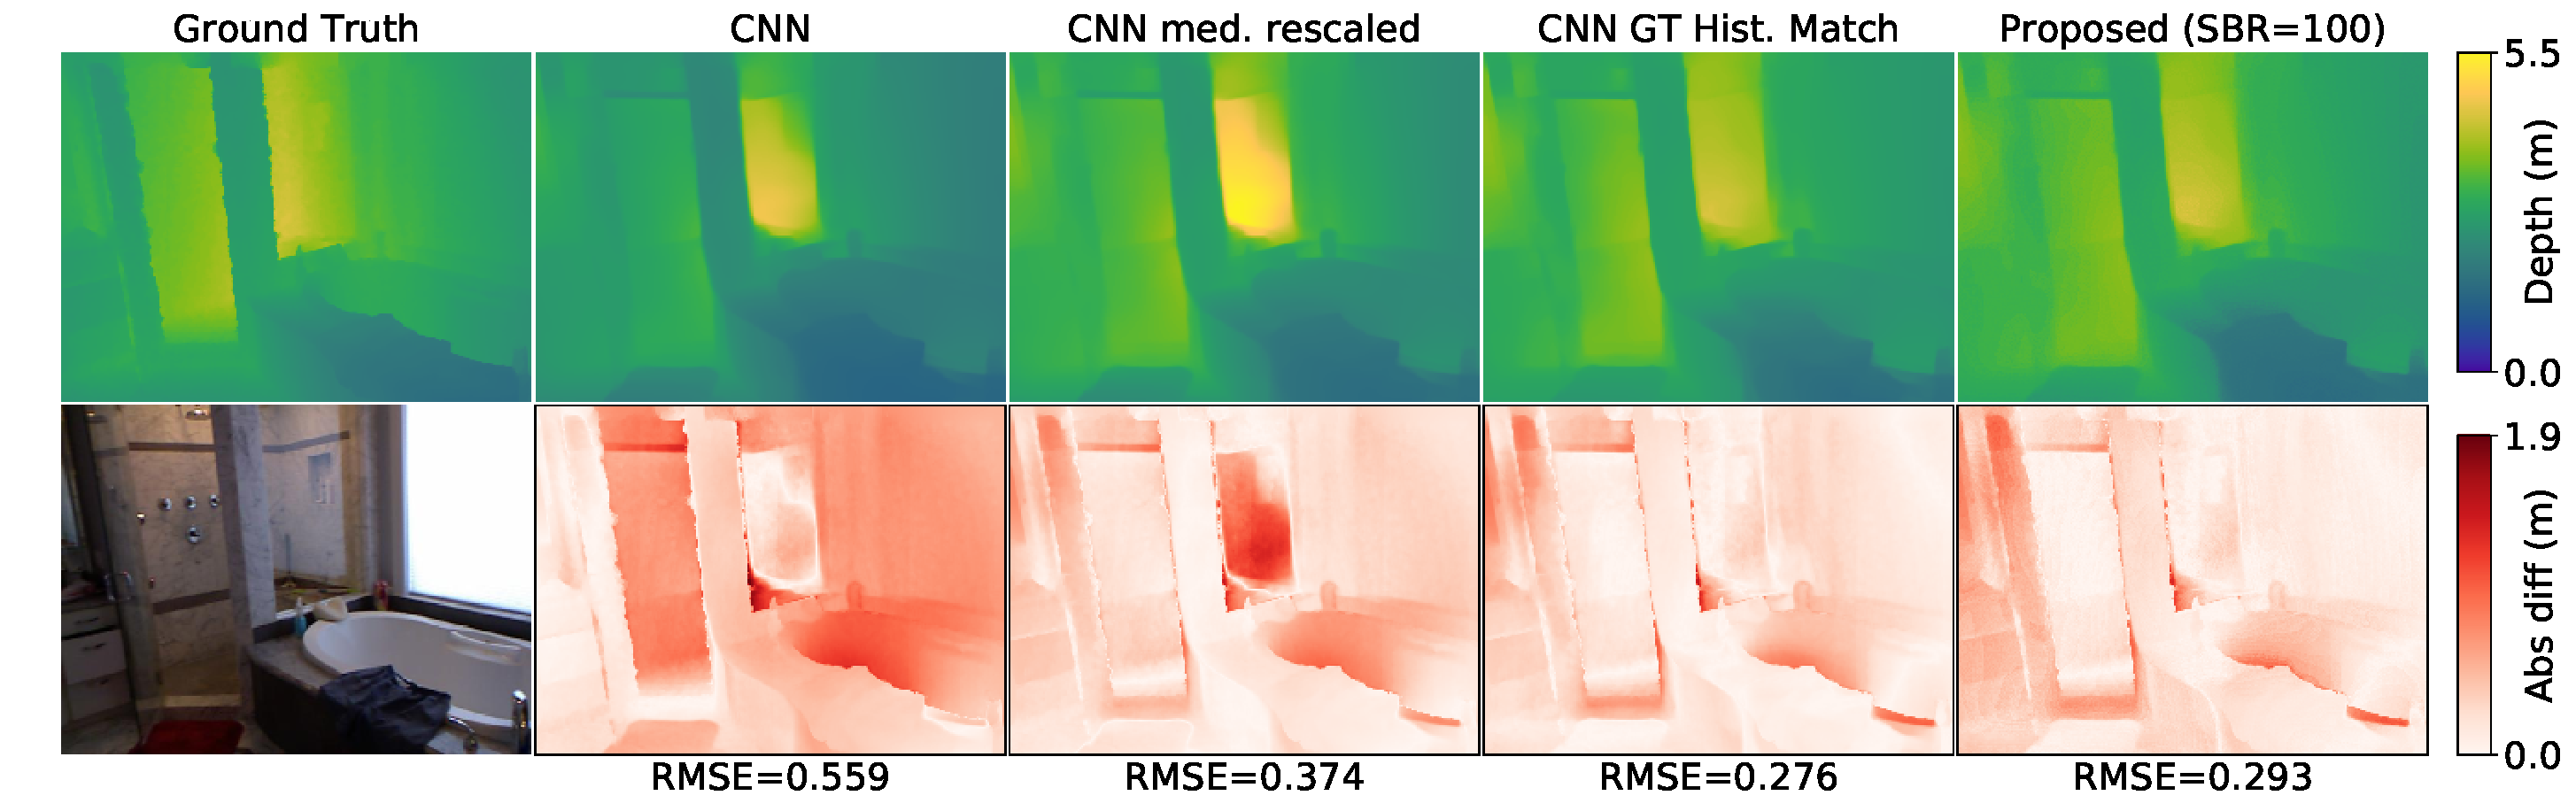
\includegraphics[width=\textwidth]{comparison/densedepth_285_comparison.pdf}
  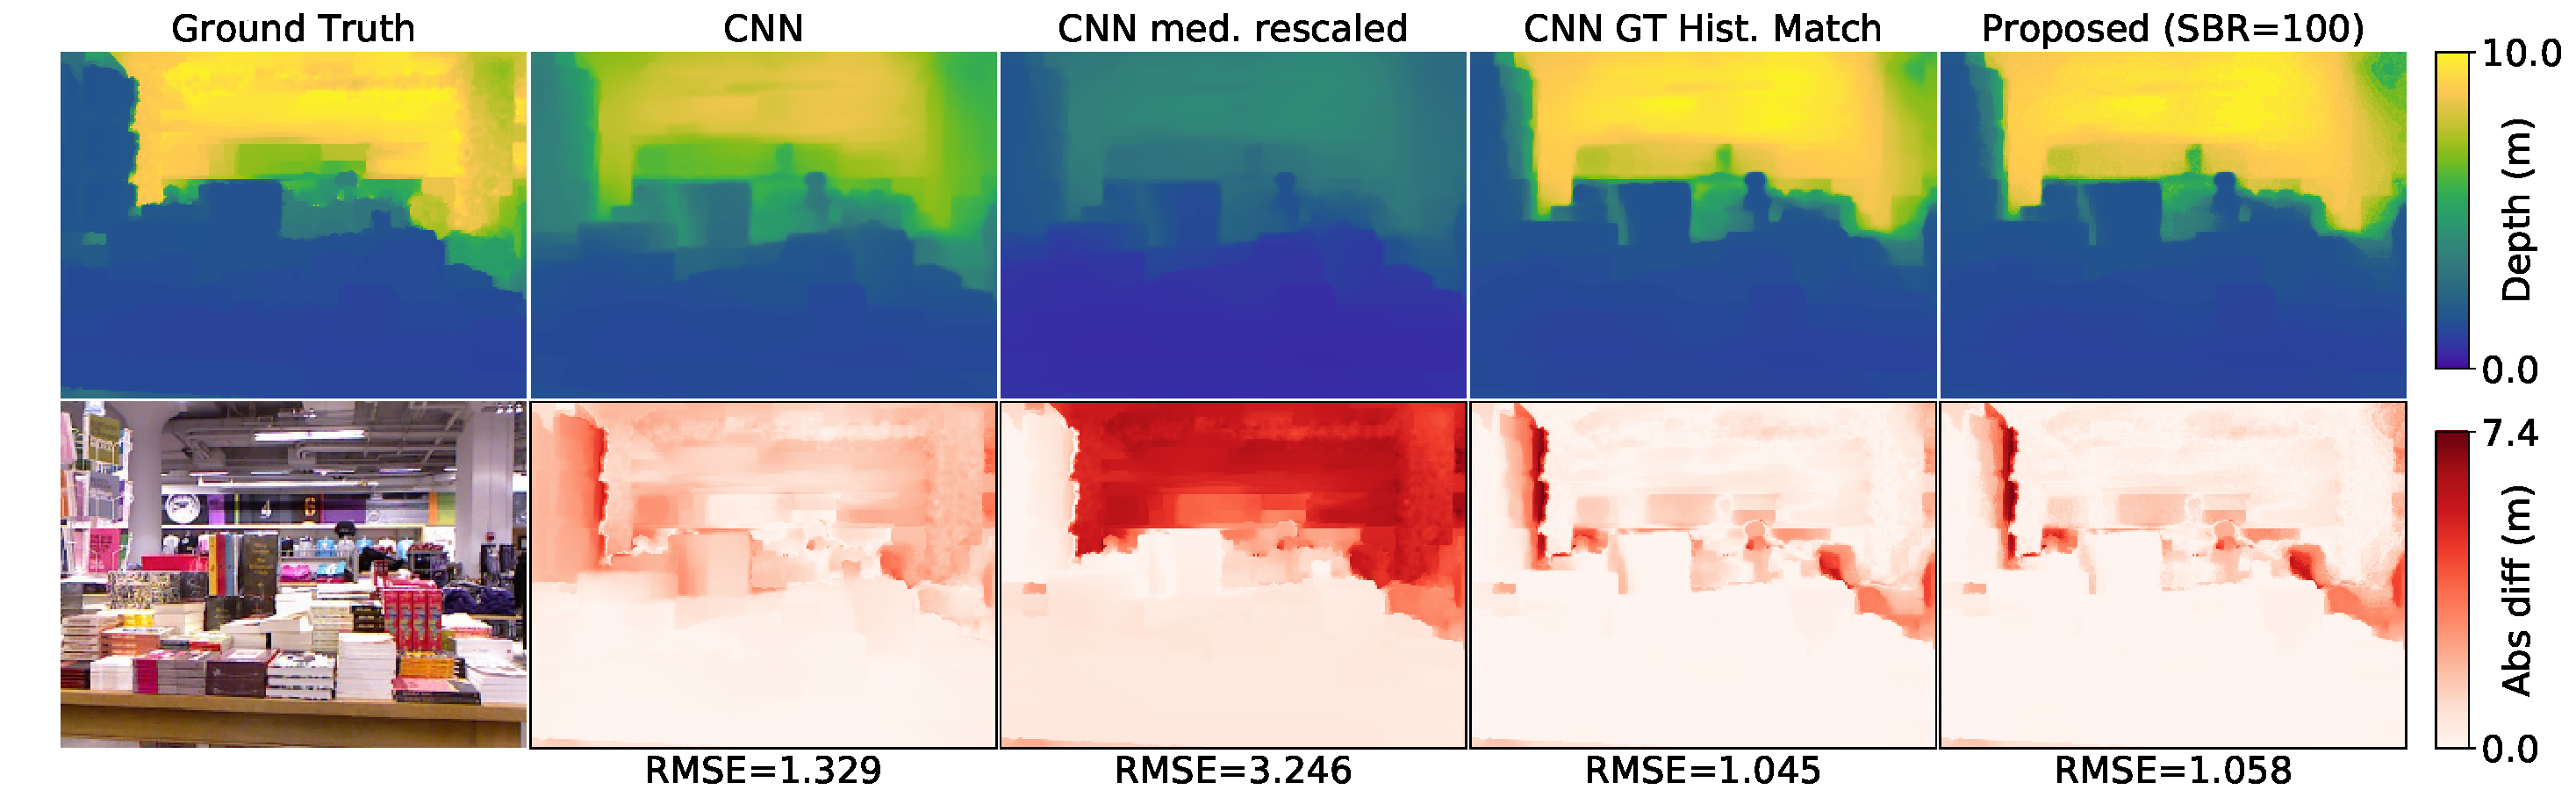
\includegraphics[width=\textwidth]{comparison/densedepth_42_comparison.pdf}
  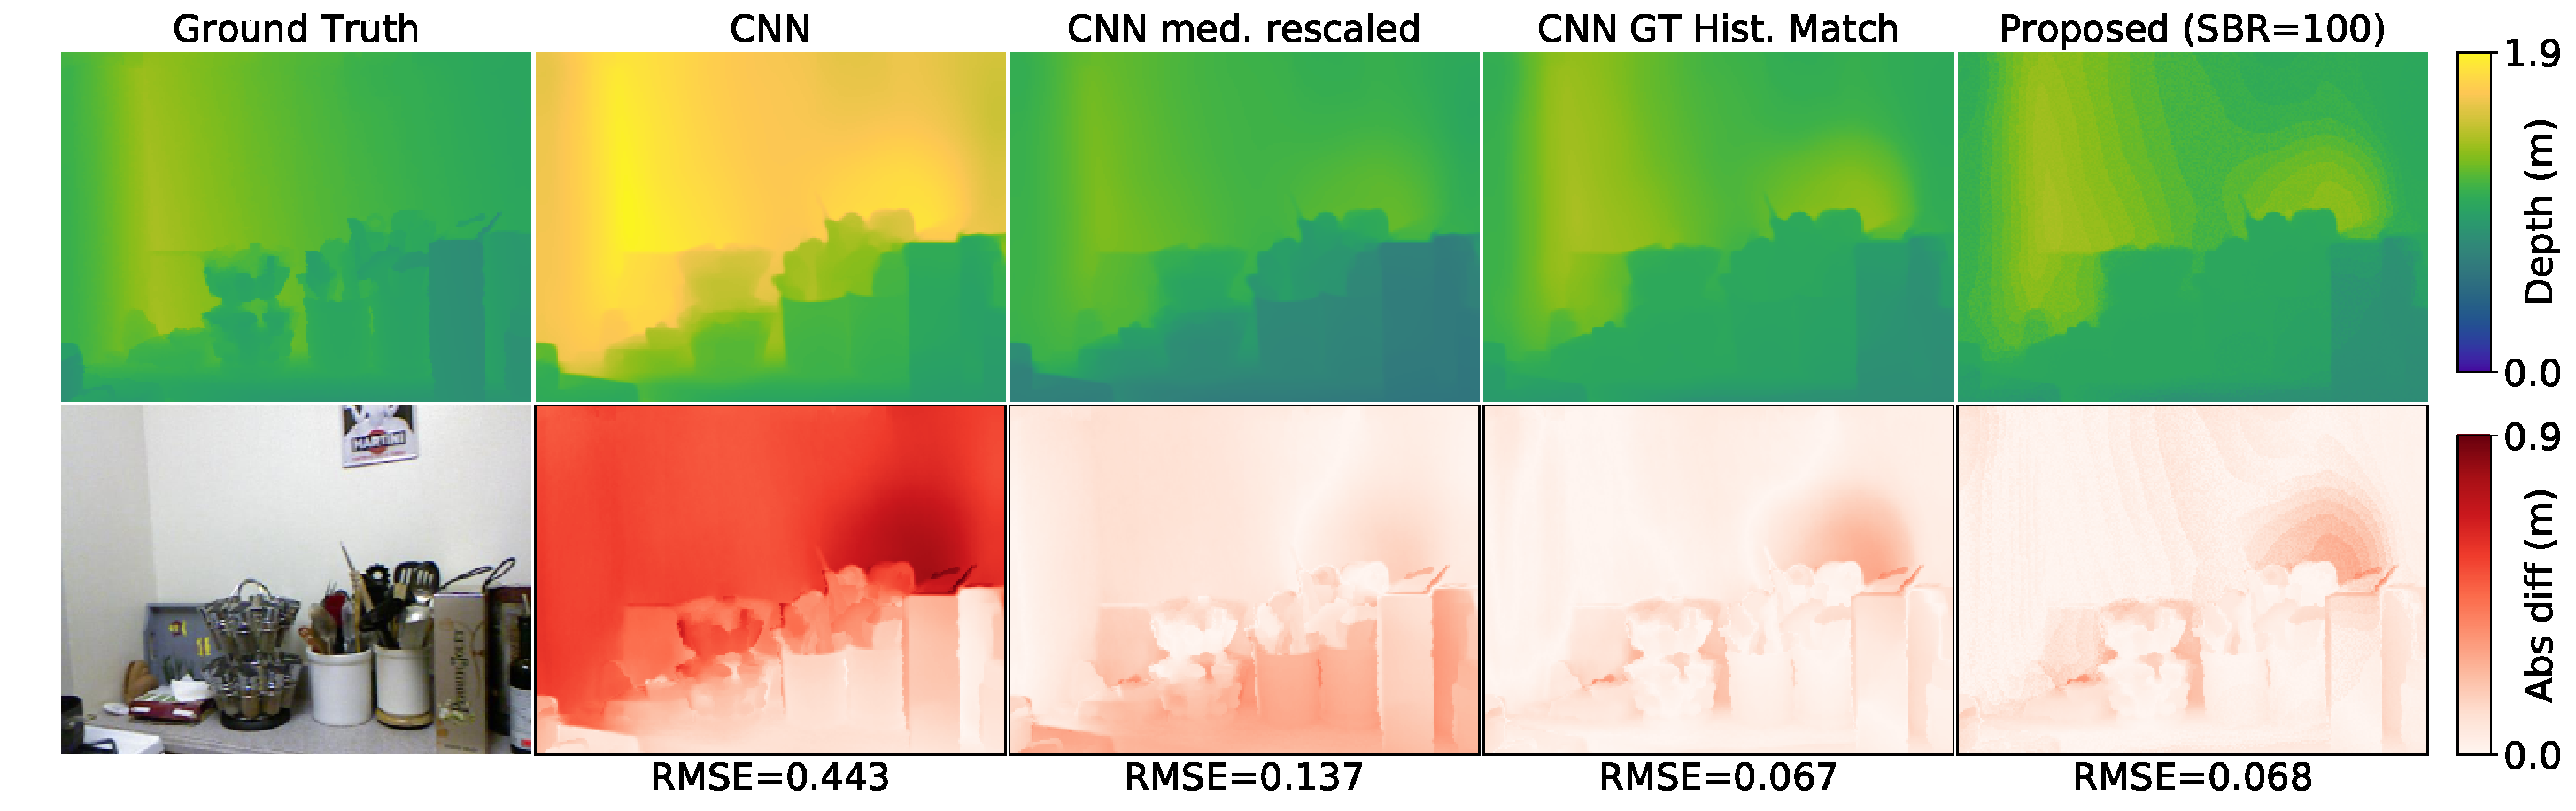
\includegraphics[width=\textwidth]{comparison/densedepth_52_comparison.pdf}
  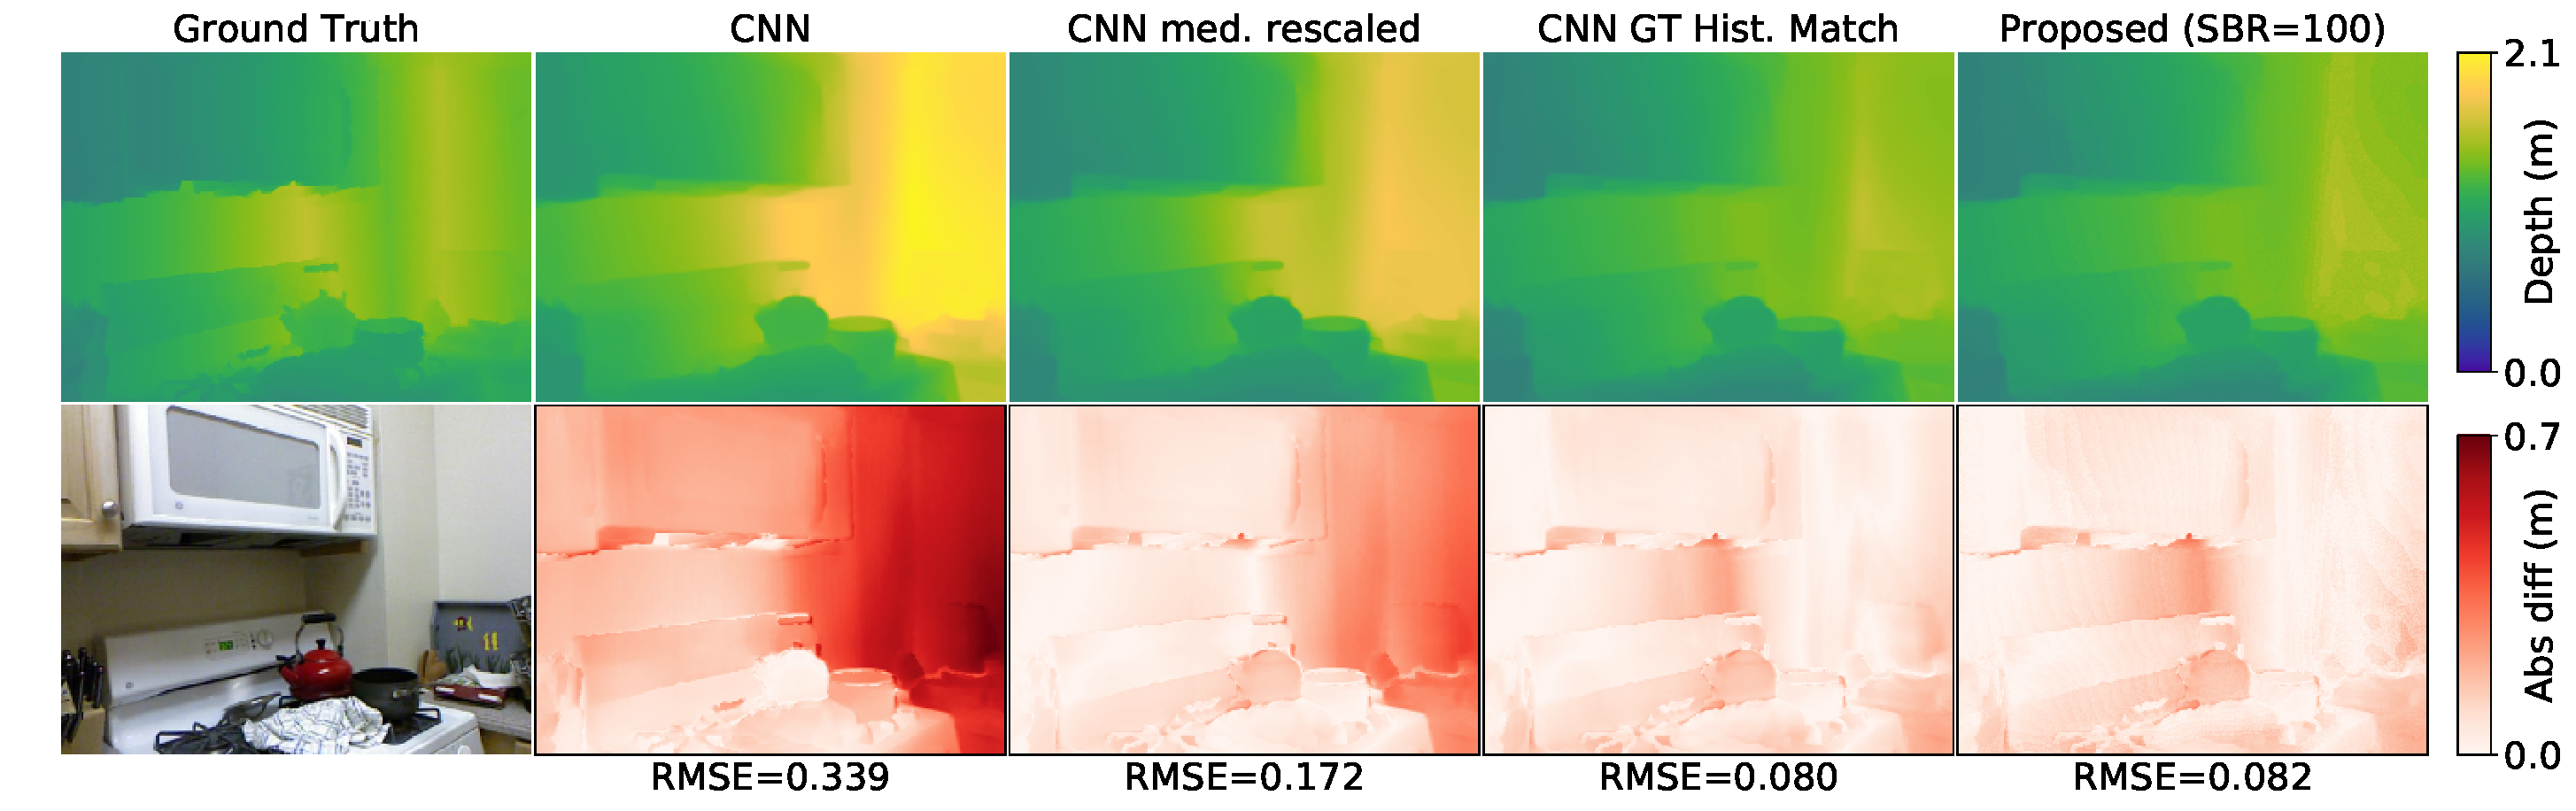
\includegraphics[width=\textwidth]{comparison/densedepth_53_comparison.pdf}
  \caption{Results with DenseDepth as the monocular depth estimator. Our method is able to scale and
    shift the depth maps to mitigate gross errors in depth scaling.}
  \label{fig:densedepth_2}
\end{figure}
\begin{figure}[H]
  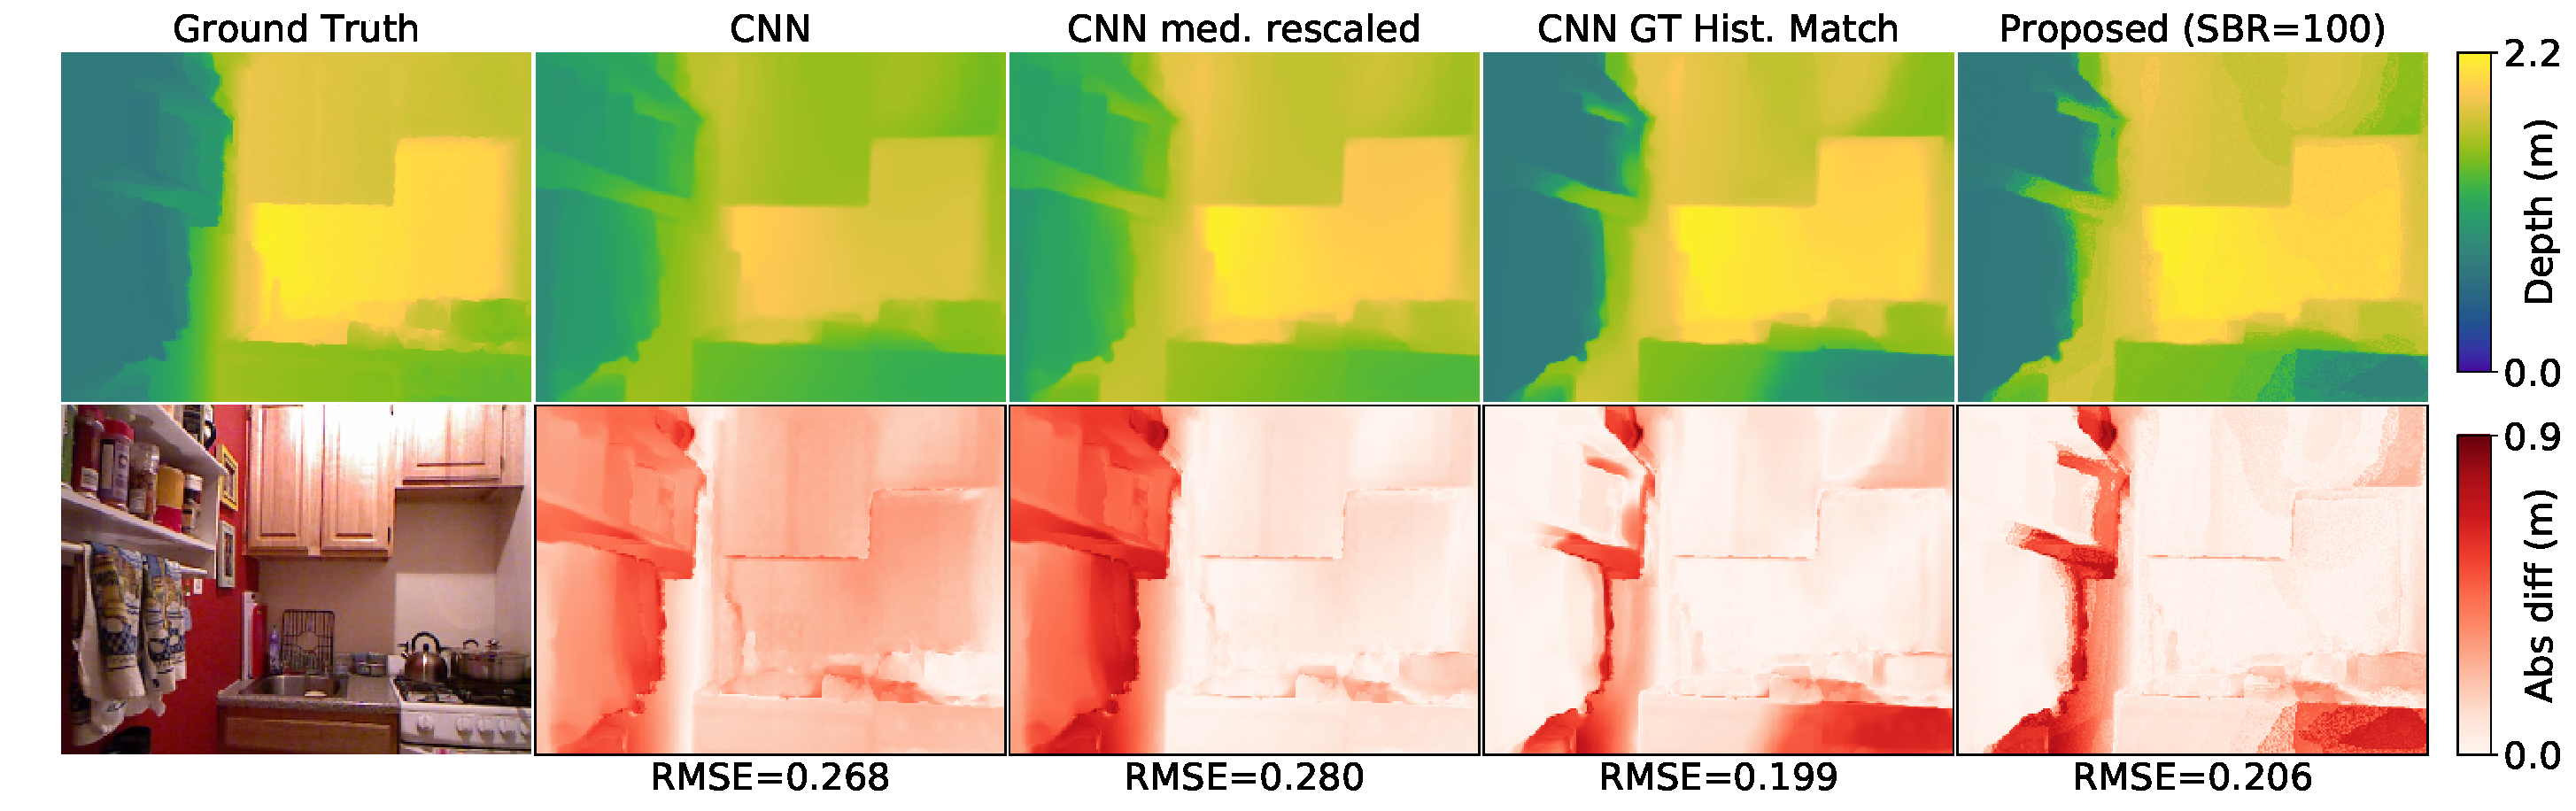
\includegraphics[width=\textwidth]{comparison/densedepth_103_comparison.pdf}
  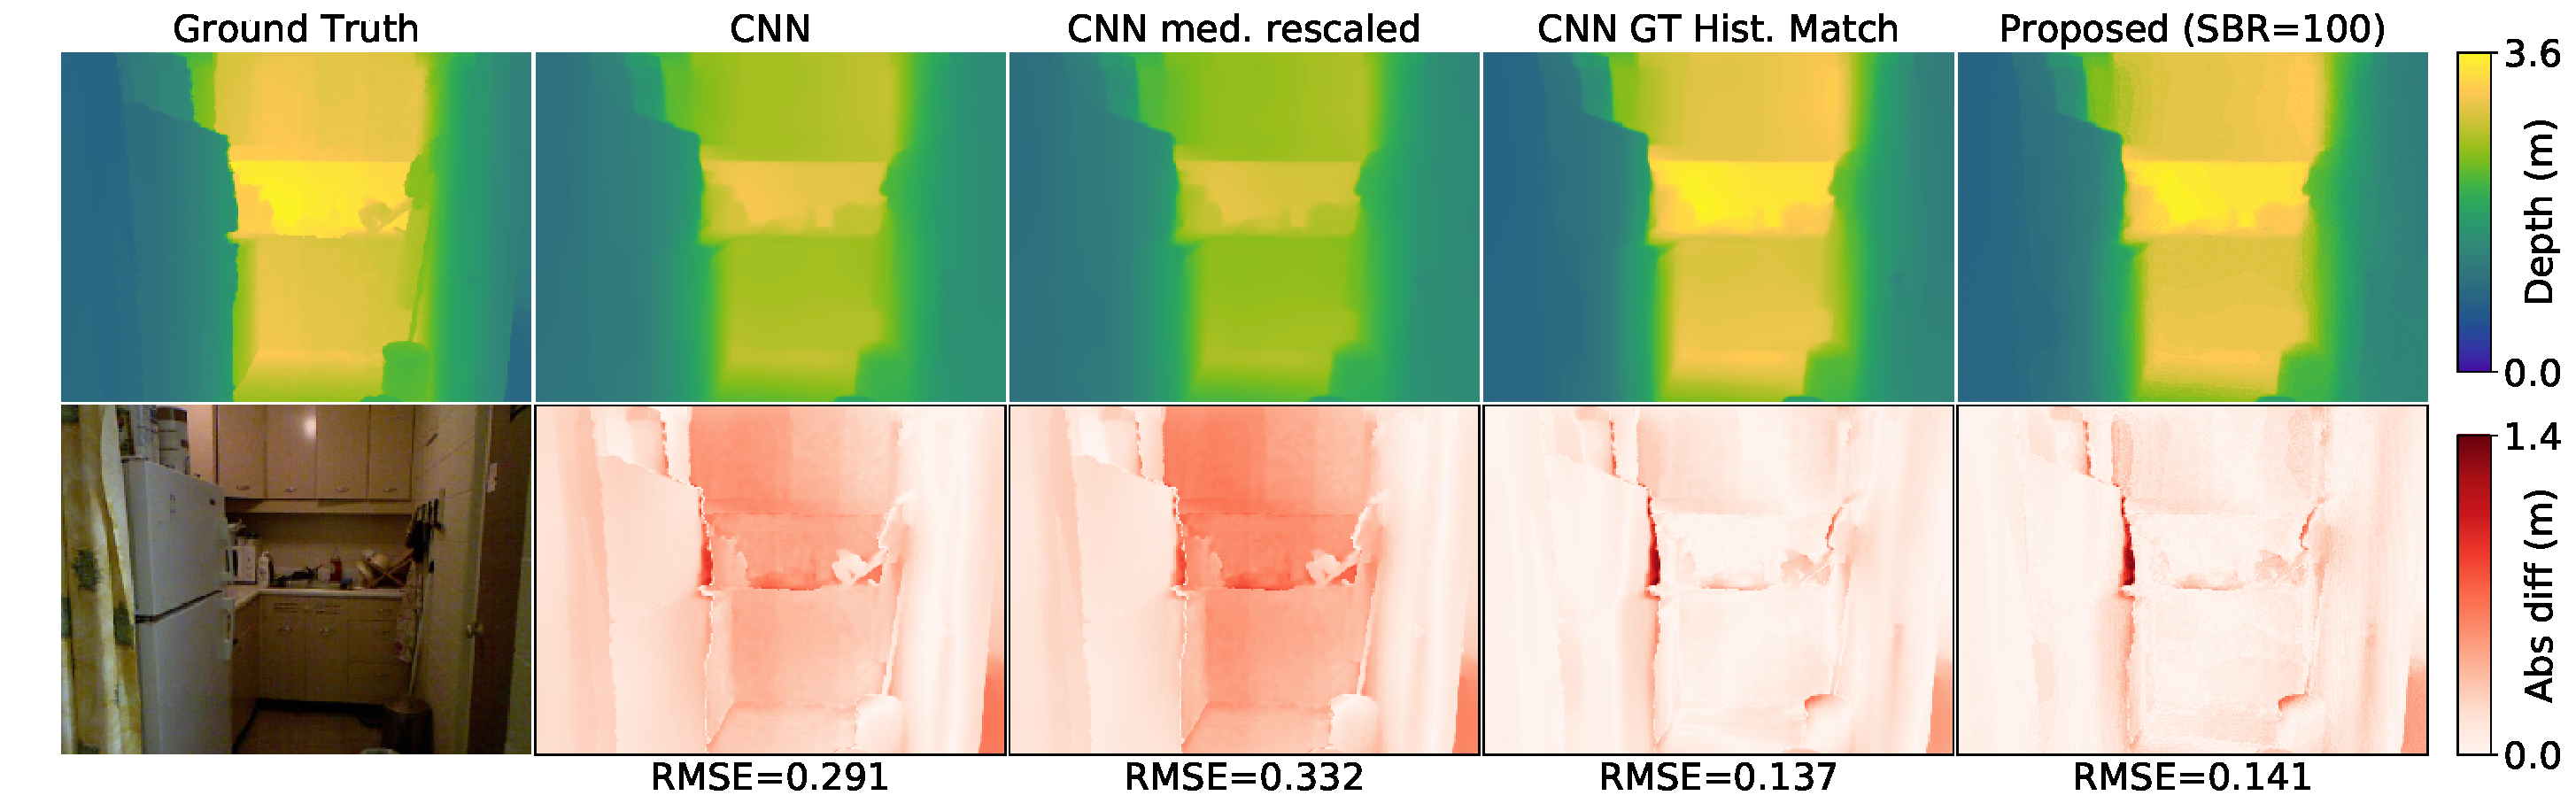
\includegraphics[width=\textwidth]{comparison/densedepth_224_comparison.pdf}
  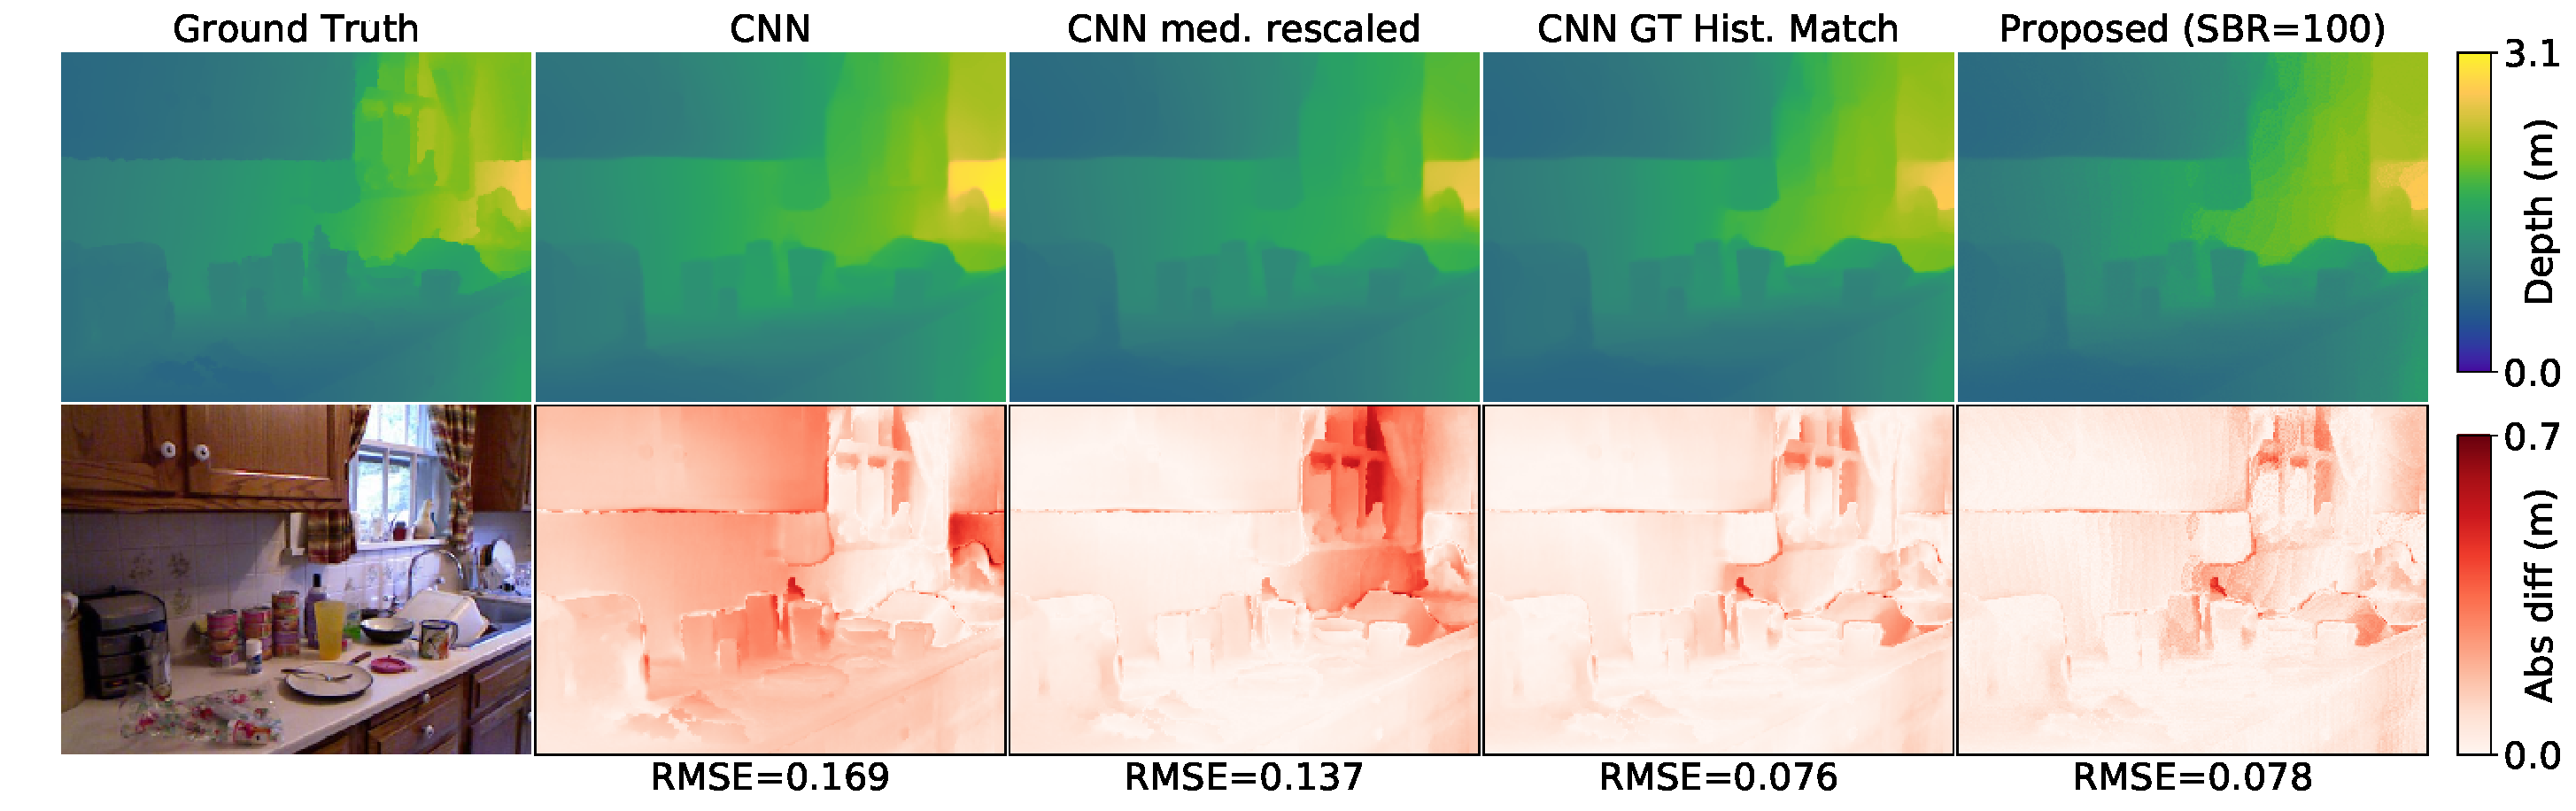
\includegraphics[width=\textwidth]{comparison/densedepth_226_comparison.pdf}
  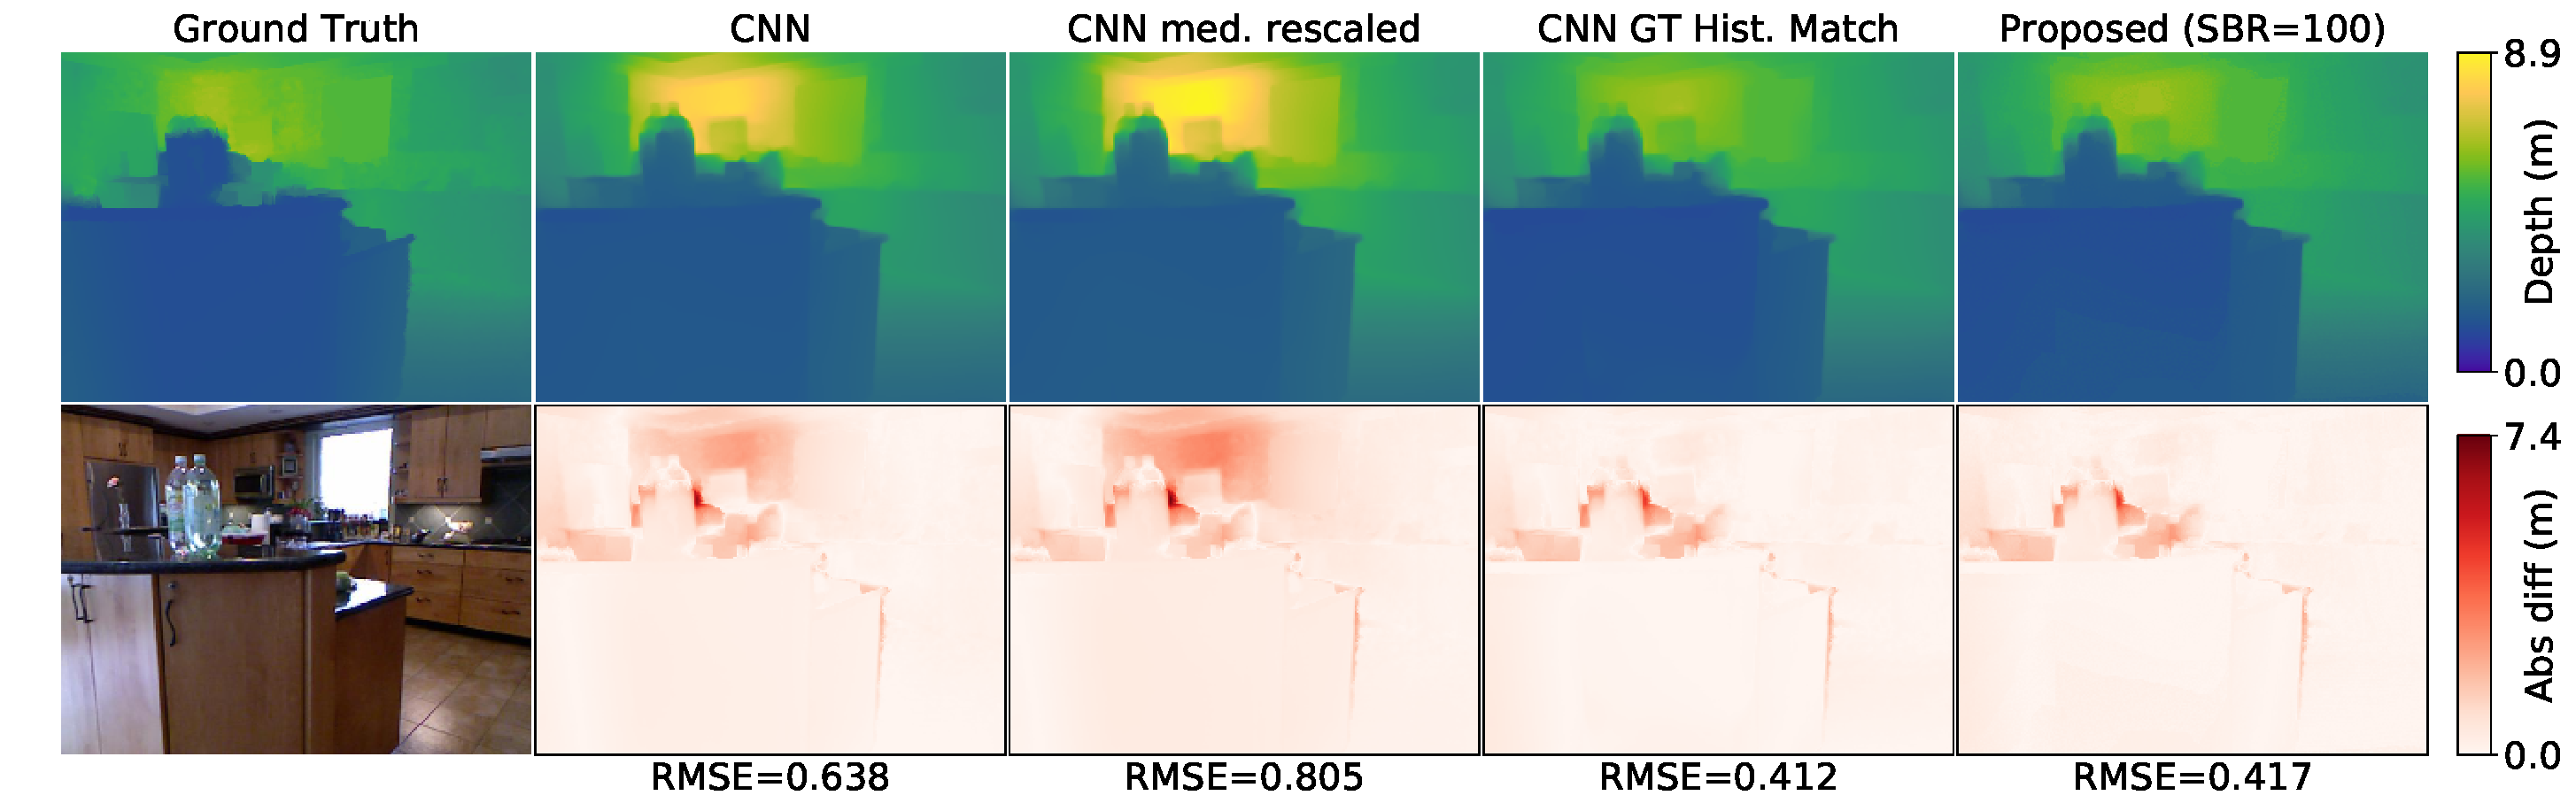
\includegraphics[width=\textwidth]{comparison/densedepth_352_comparison.pdf}
  \caption{Results with DenseDepth as the monocular depth estimator. Our method is able to scale and
    shift the depth maps to mitigate gross errors in depth scaling.}
  \label{fig:densedepth_3}
\end{figure}
% \begin{figure}
%   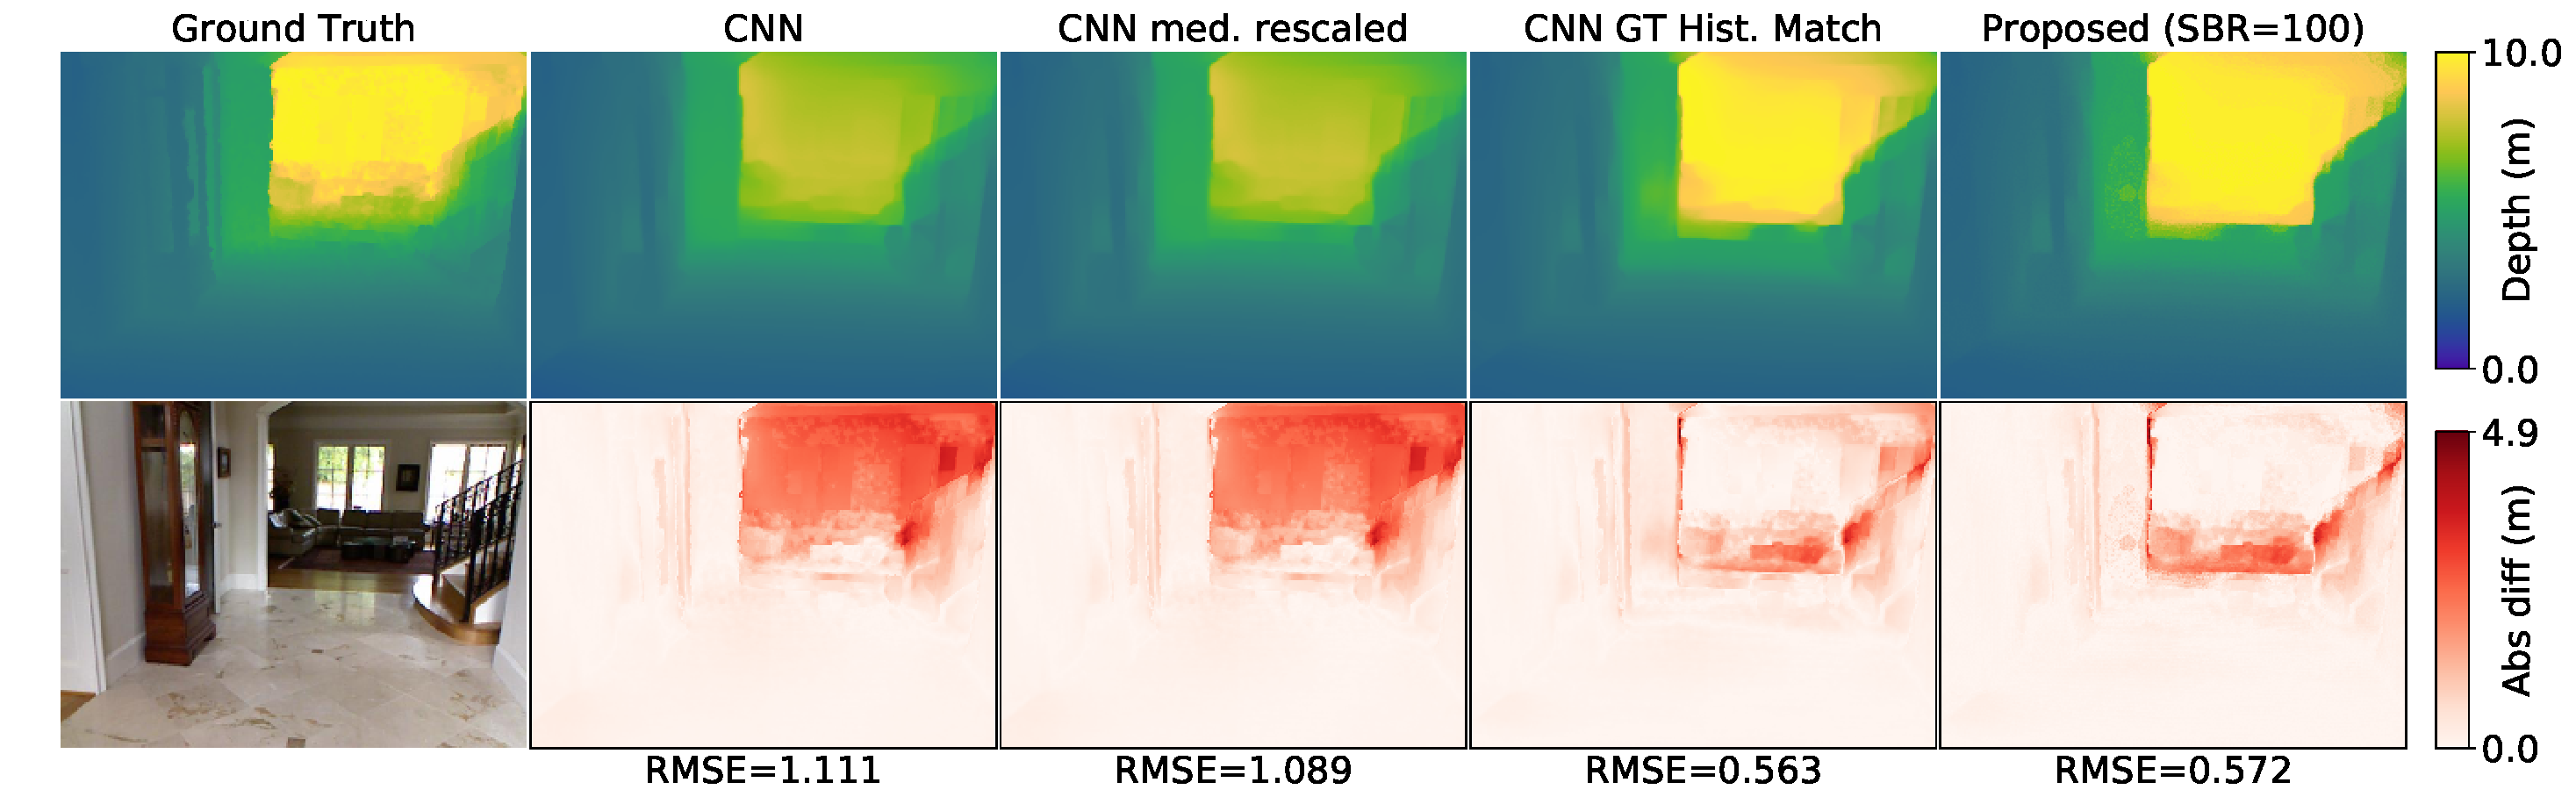
\includegraphics[width=\textwidth]{comparison/densedepth_140_comparison.pdf}
%   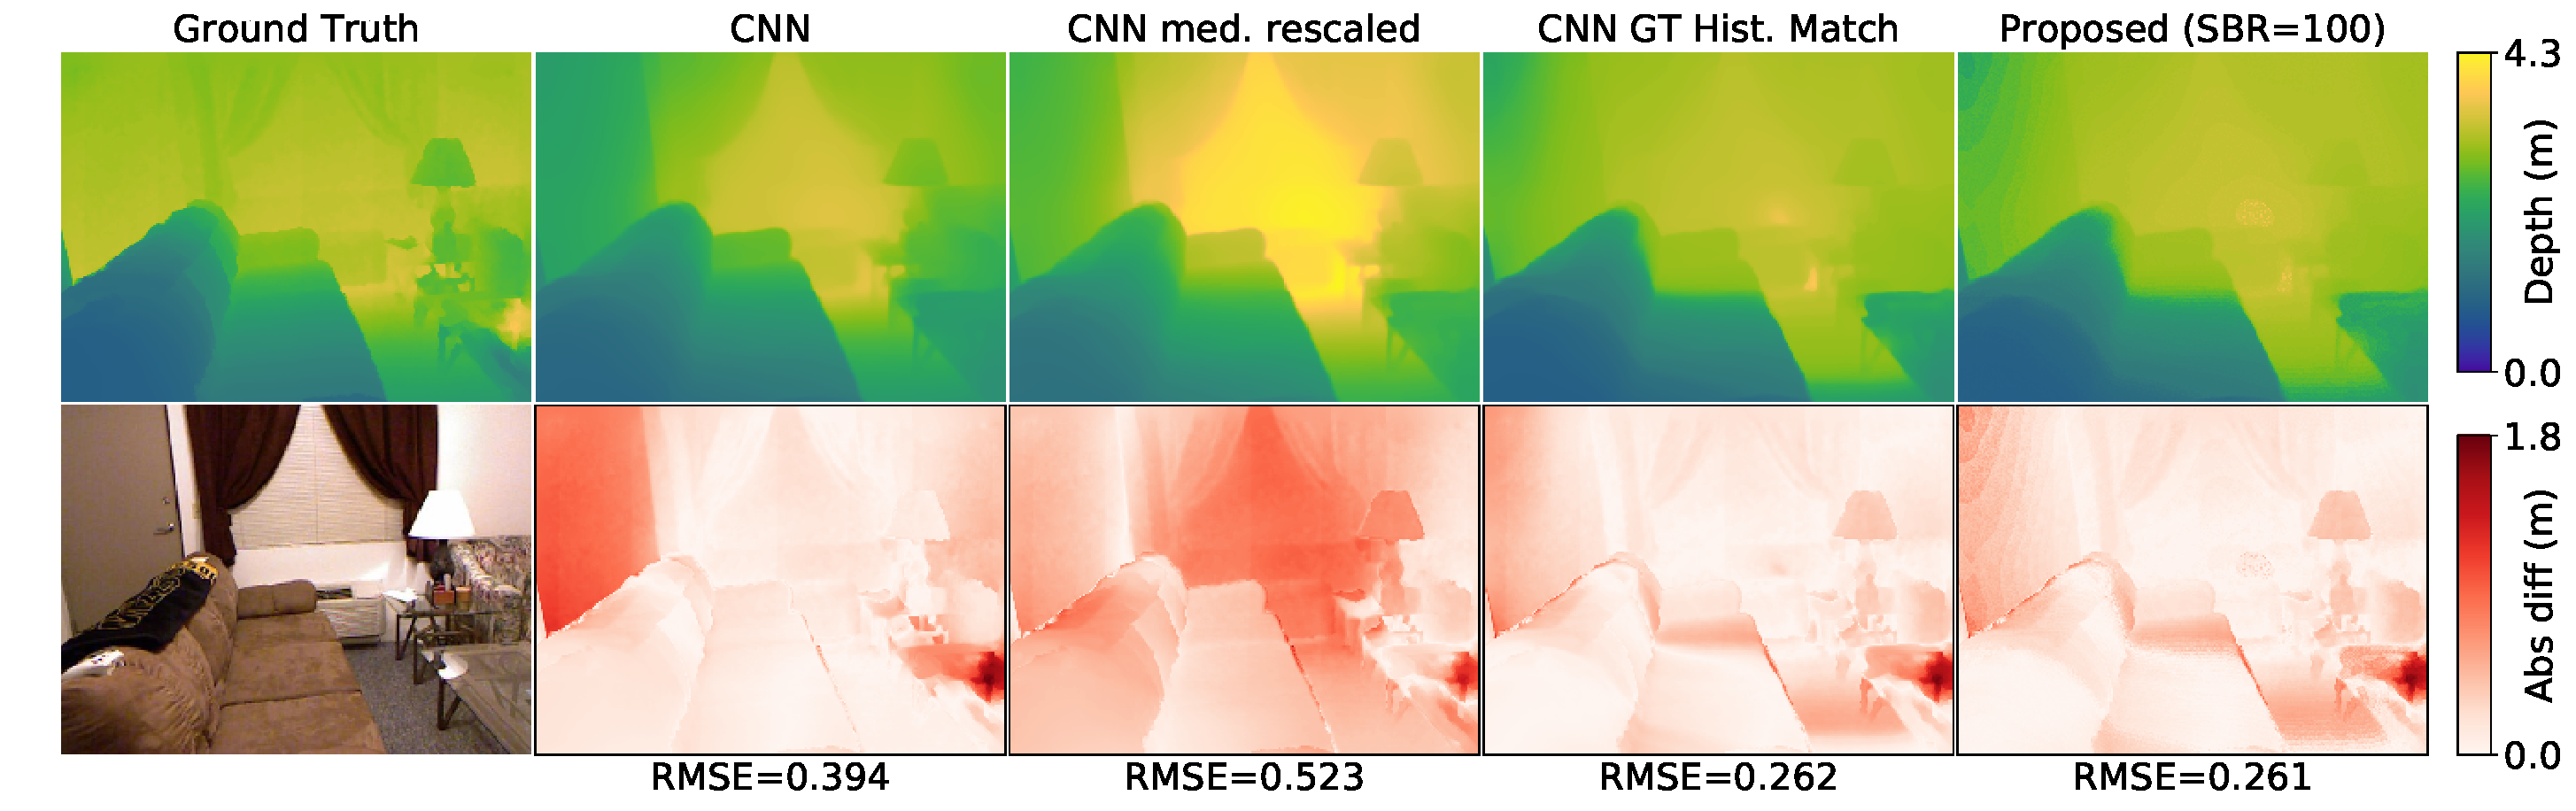
\includegraphics[width=\textwidth]{comparison/densedepth_244_comparison.pdf}
%   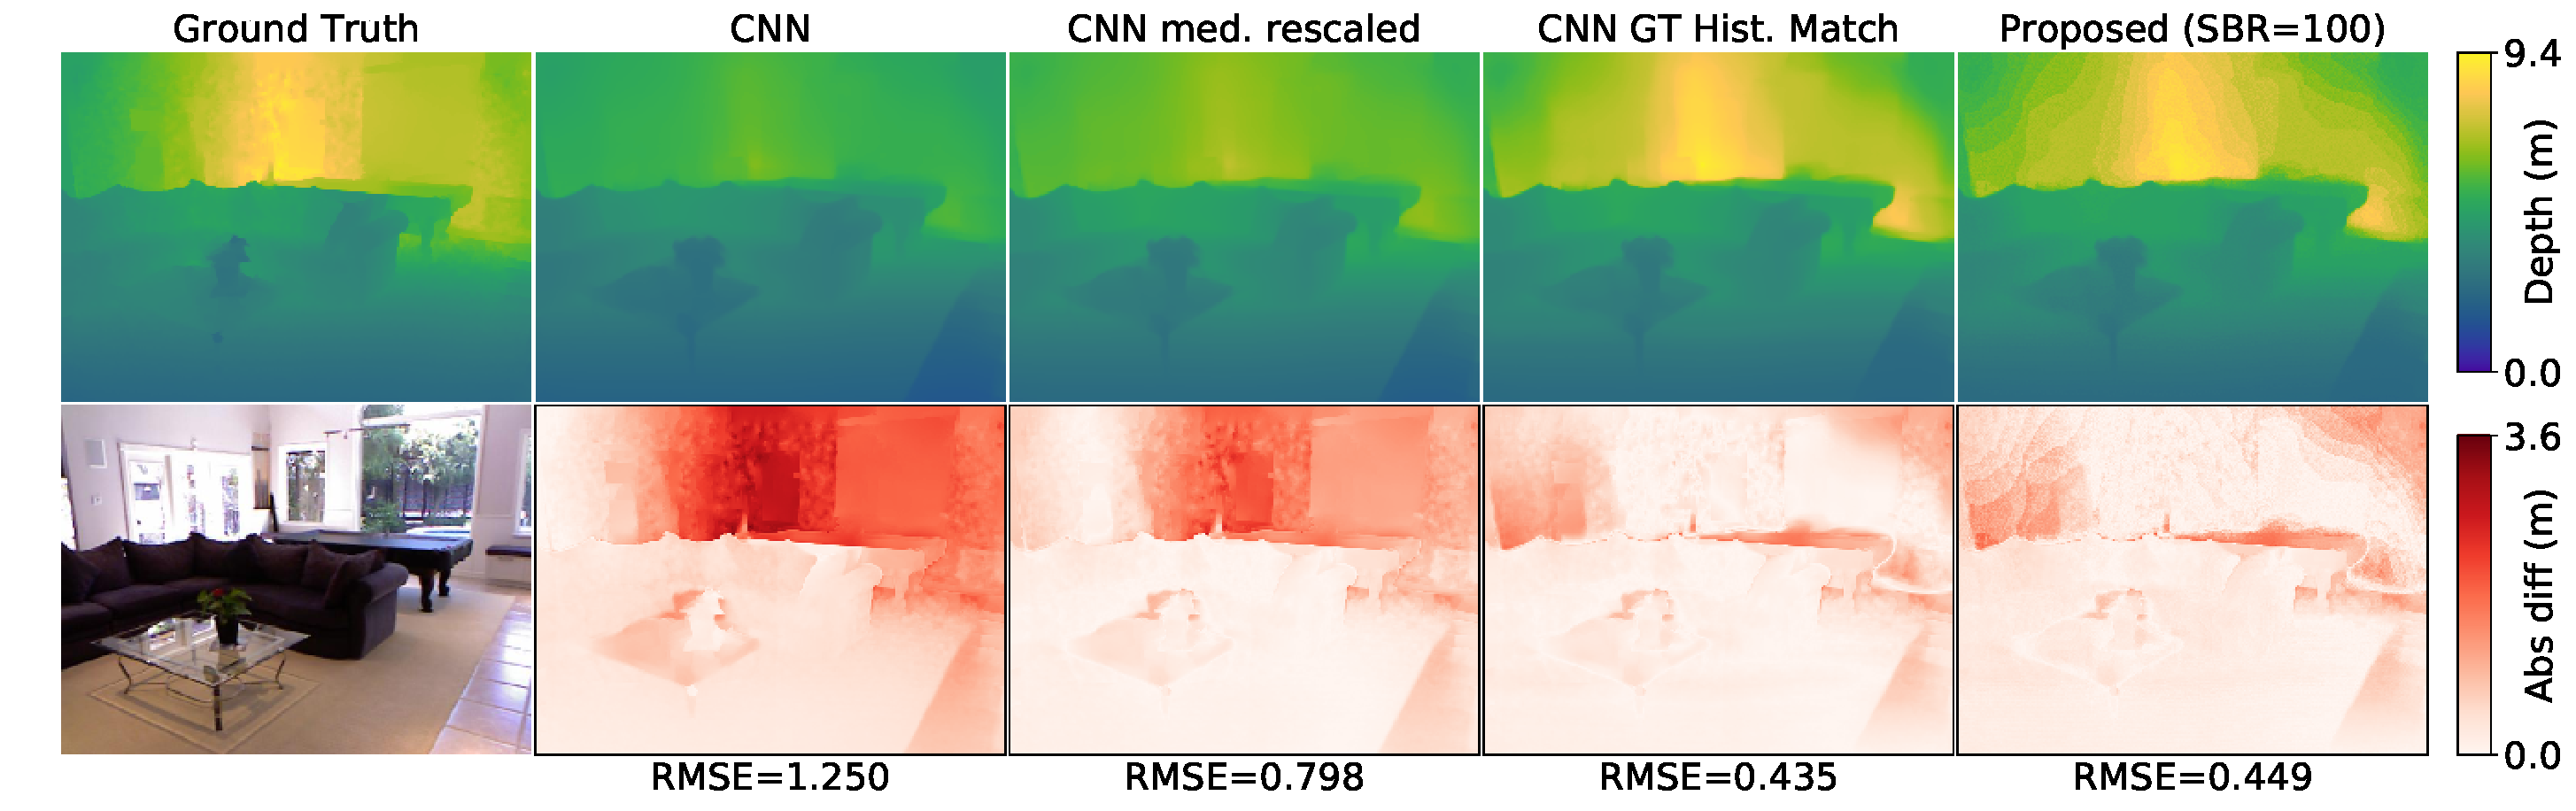
\includegraphics[width=\textwidth]{comparison/densedepth_527_comparison.pdf}
%   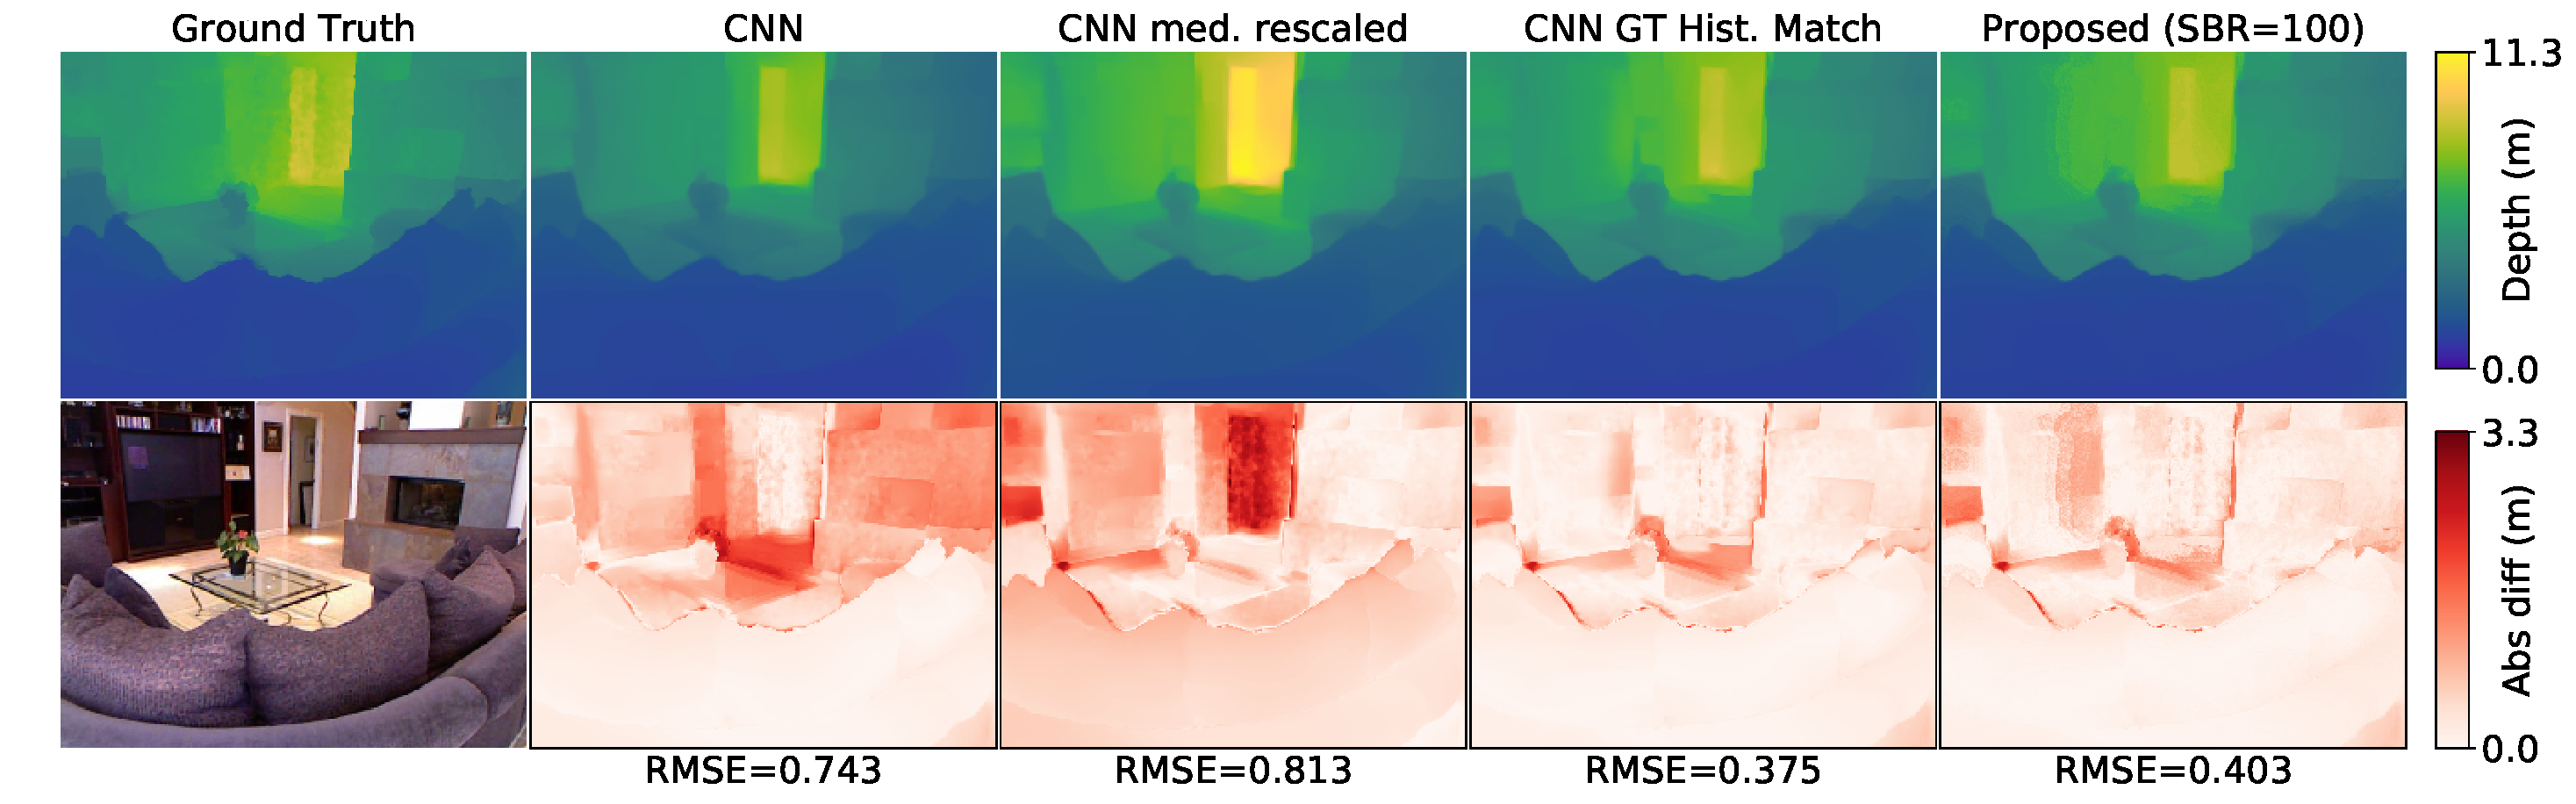
\includegraphics[width=\textwidth]{comparison/densedepth_529_comparison.pdf}
%   \caption{Results on DenseDepth}
% \end{figure}
% \begin{figure}
%   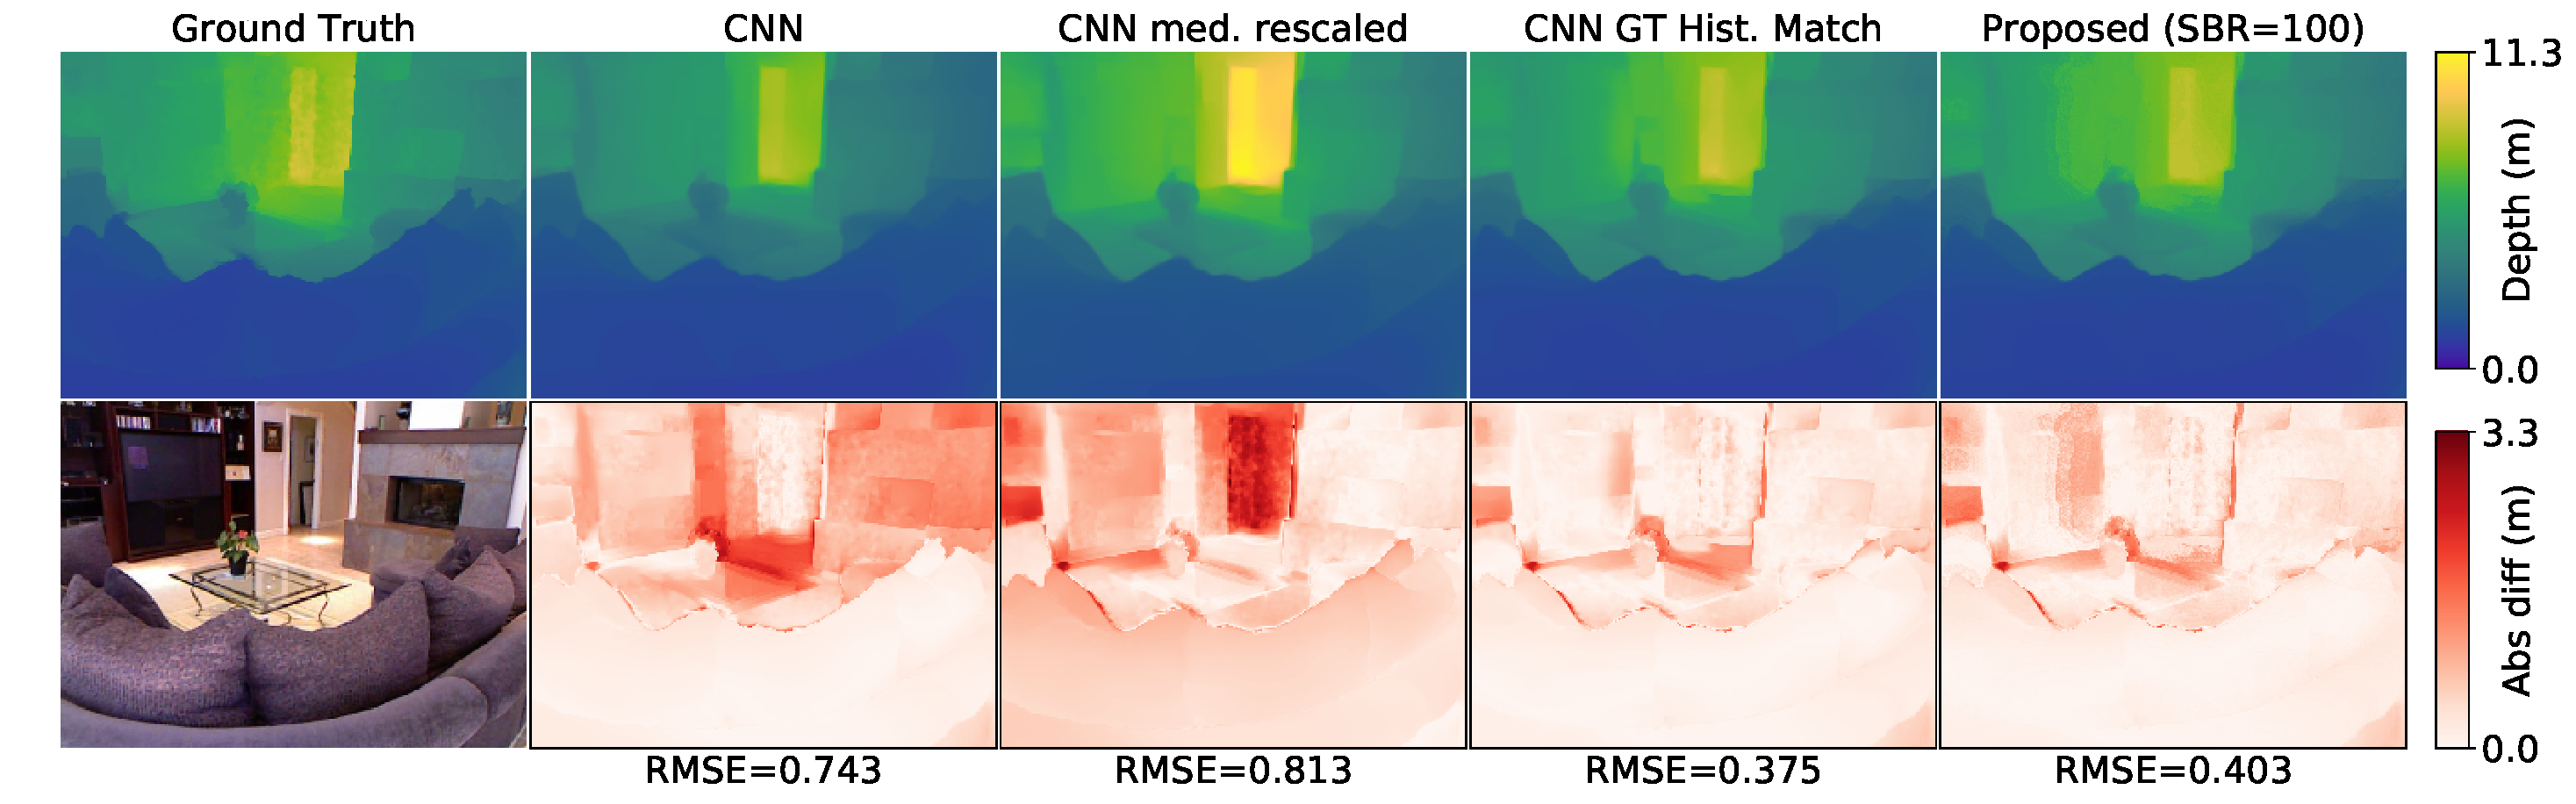
\includegraphics[width=\textwidth]{comparison/densedepth_529_comparison.pdf}
%   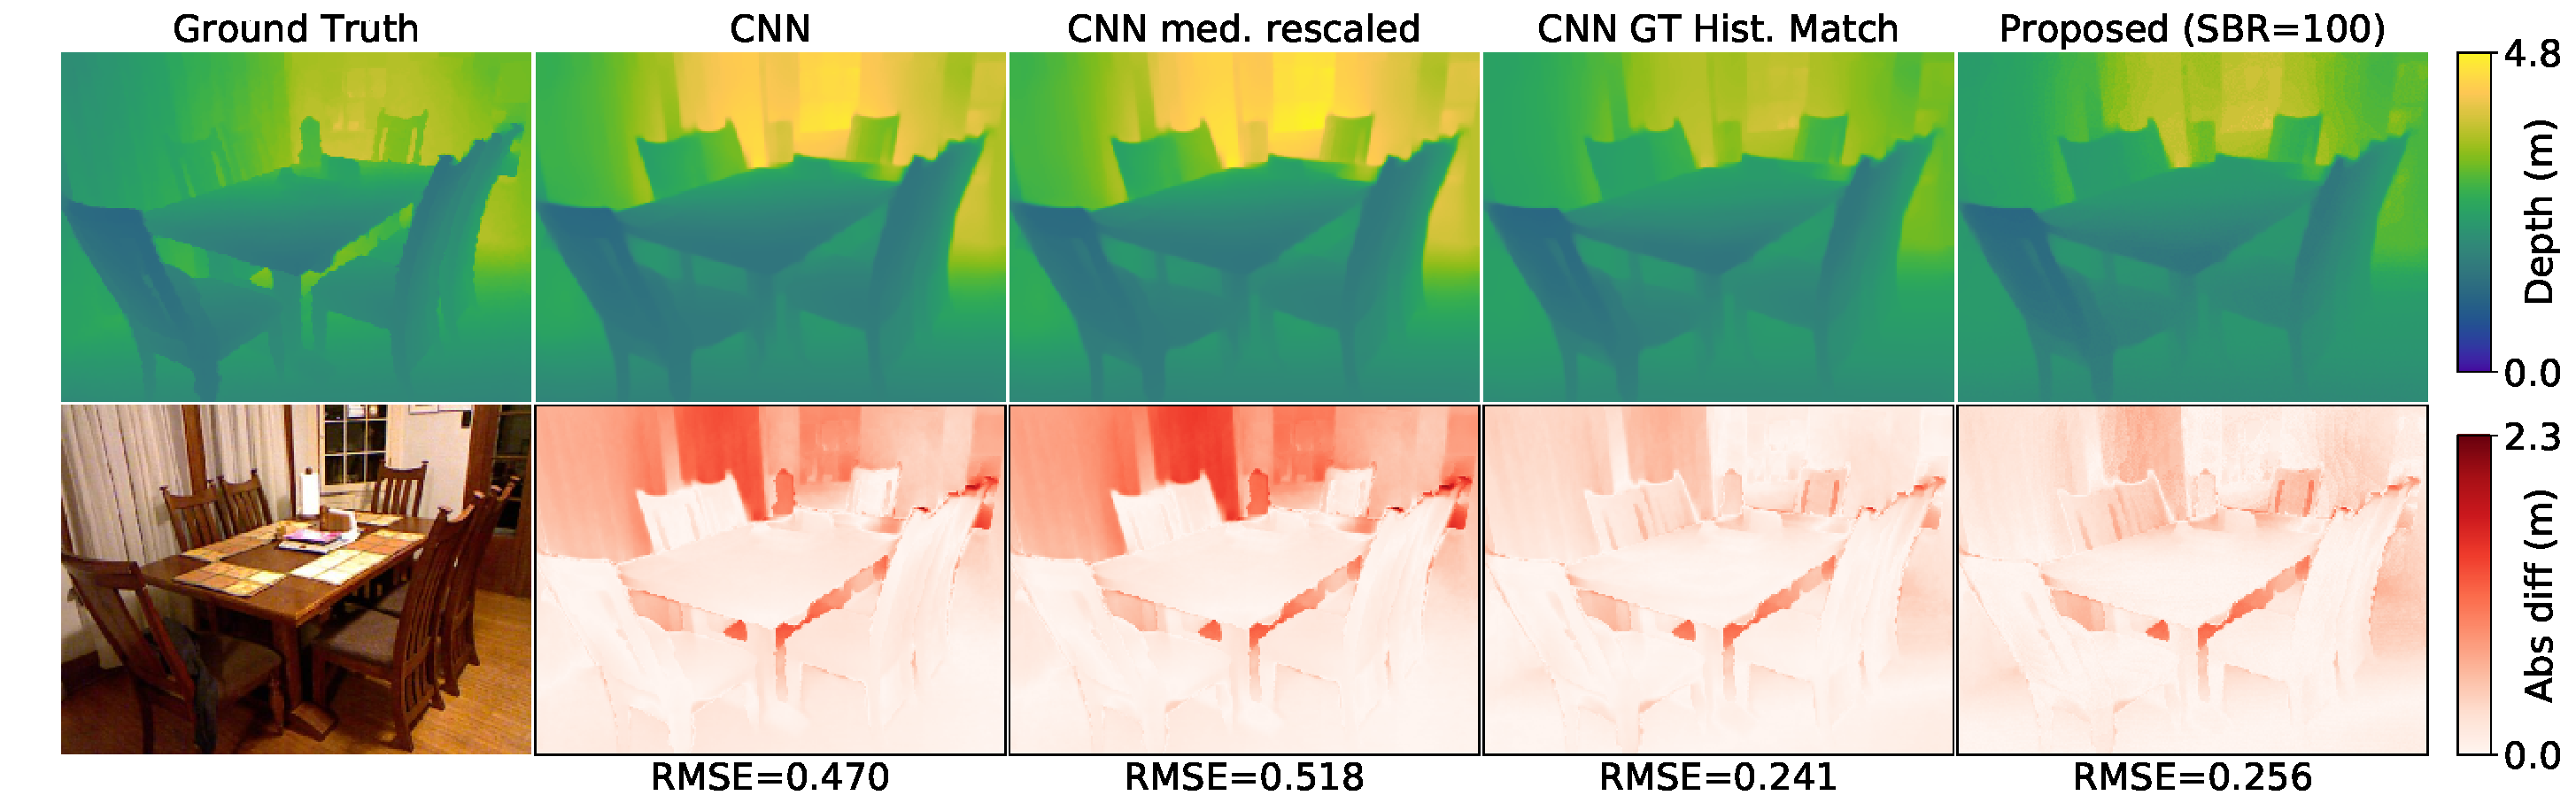
\includegraphics[width=\textwidth]{comparison/densedepth_219_comparison.pdf}
%   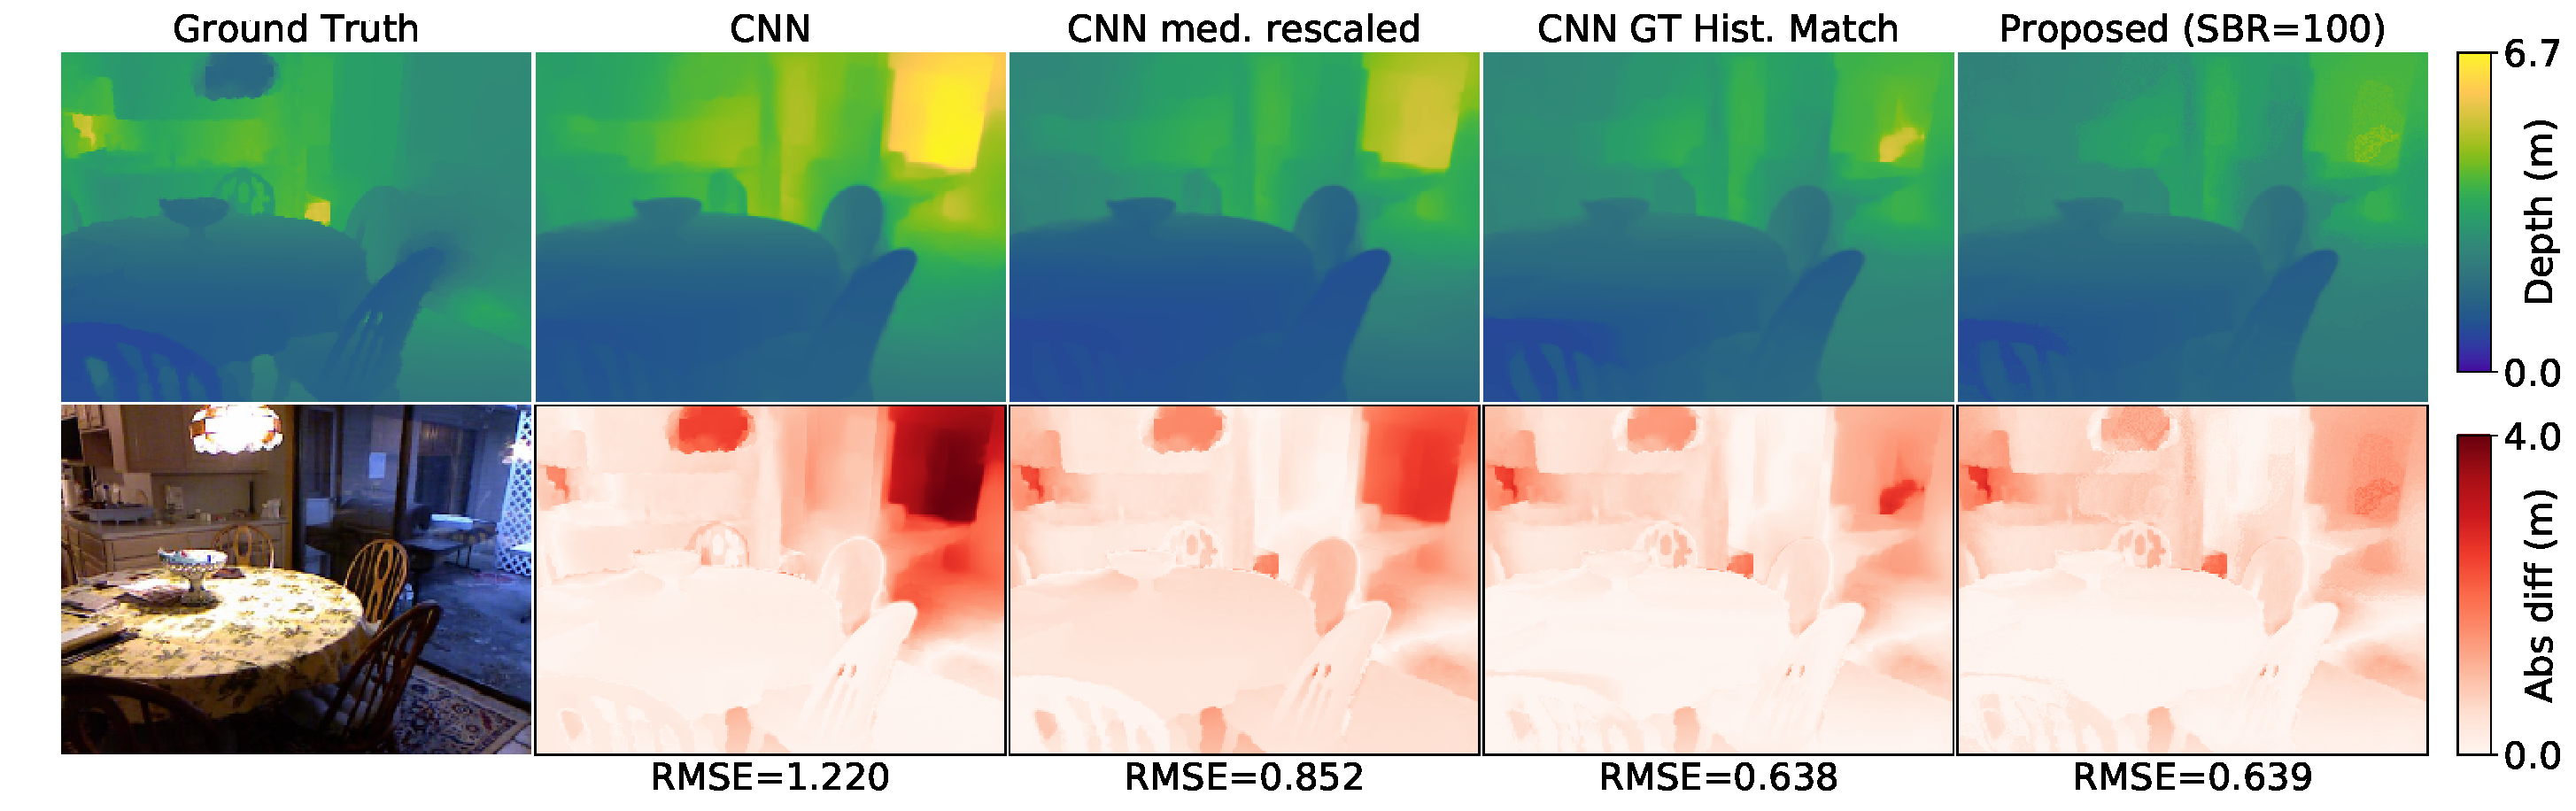
\includegraphics[width=\textwidth]{comparison/densedepth_329_comparison.pdf}
%   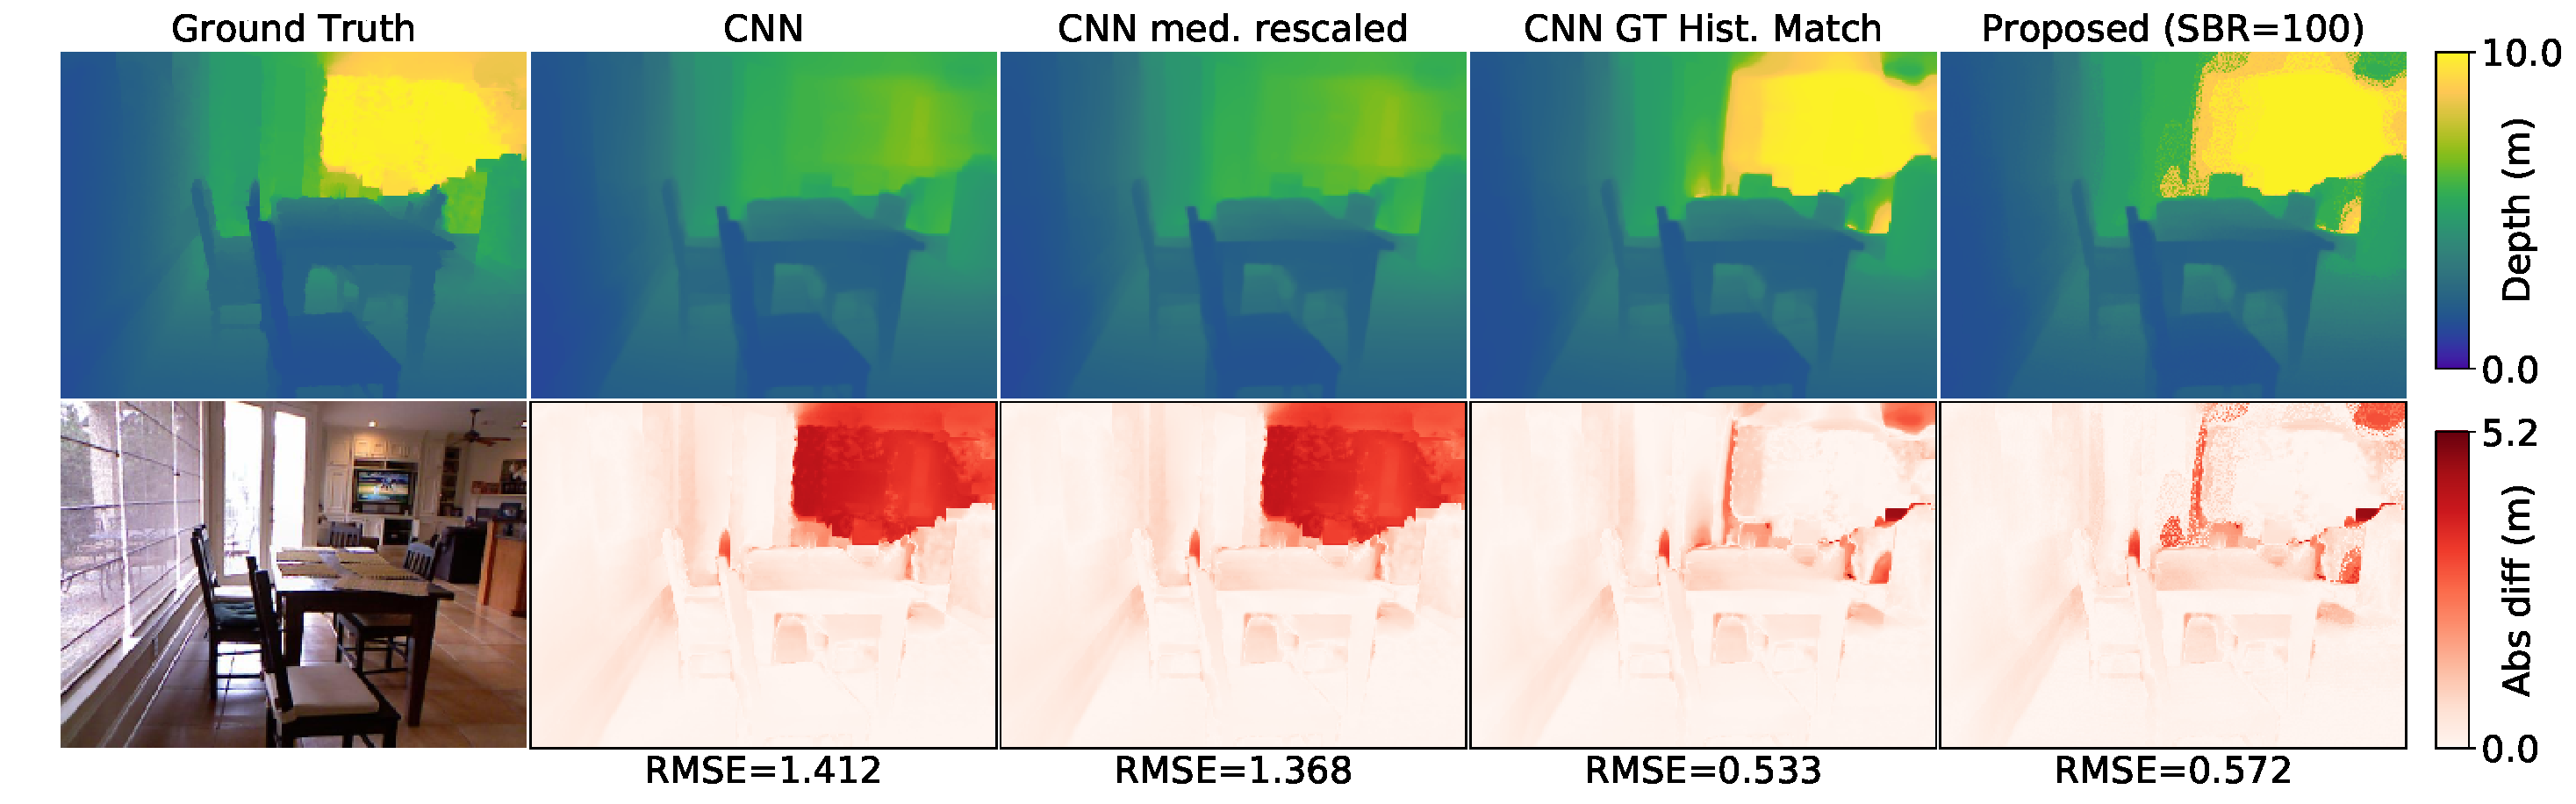
\includegraphics[width=\textwidth]{comparison/densedepth_346_comparison.pdf}
%   \caption{Results on DenseDepth}
% \end{figure}
% \begin{figure}
%   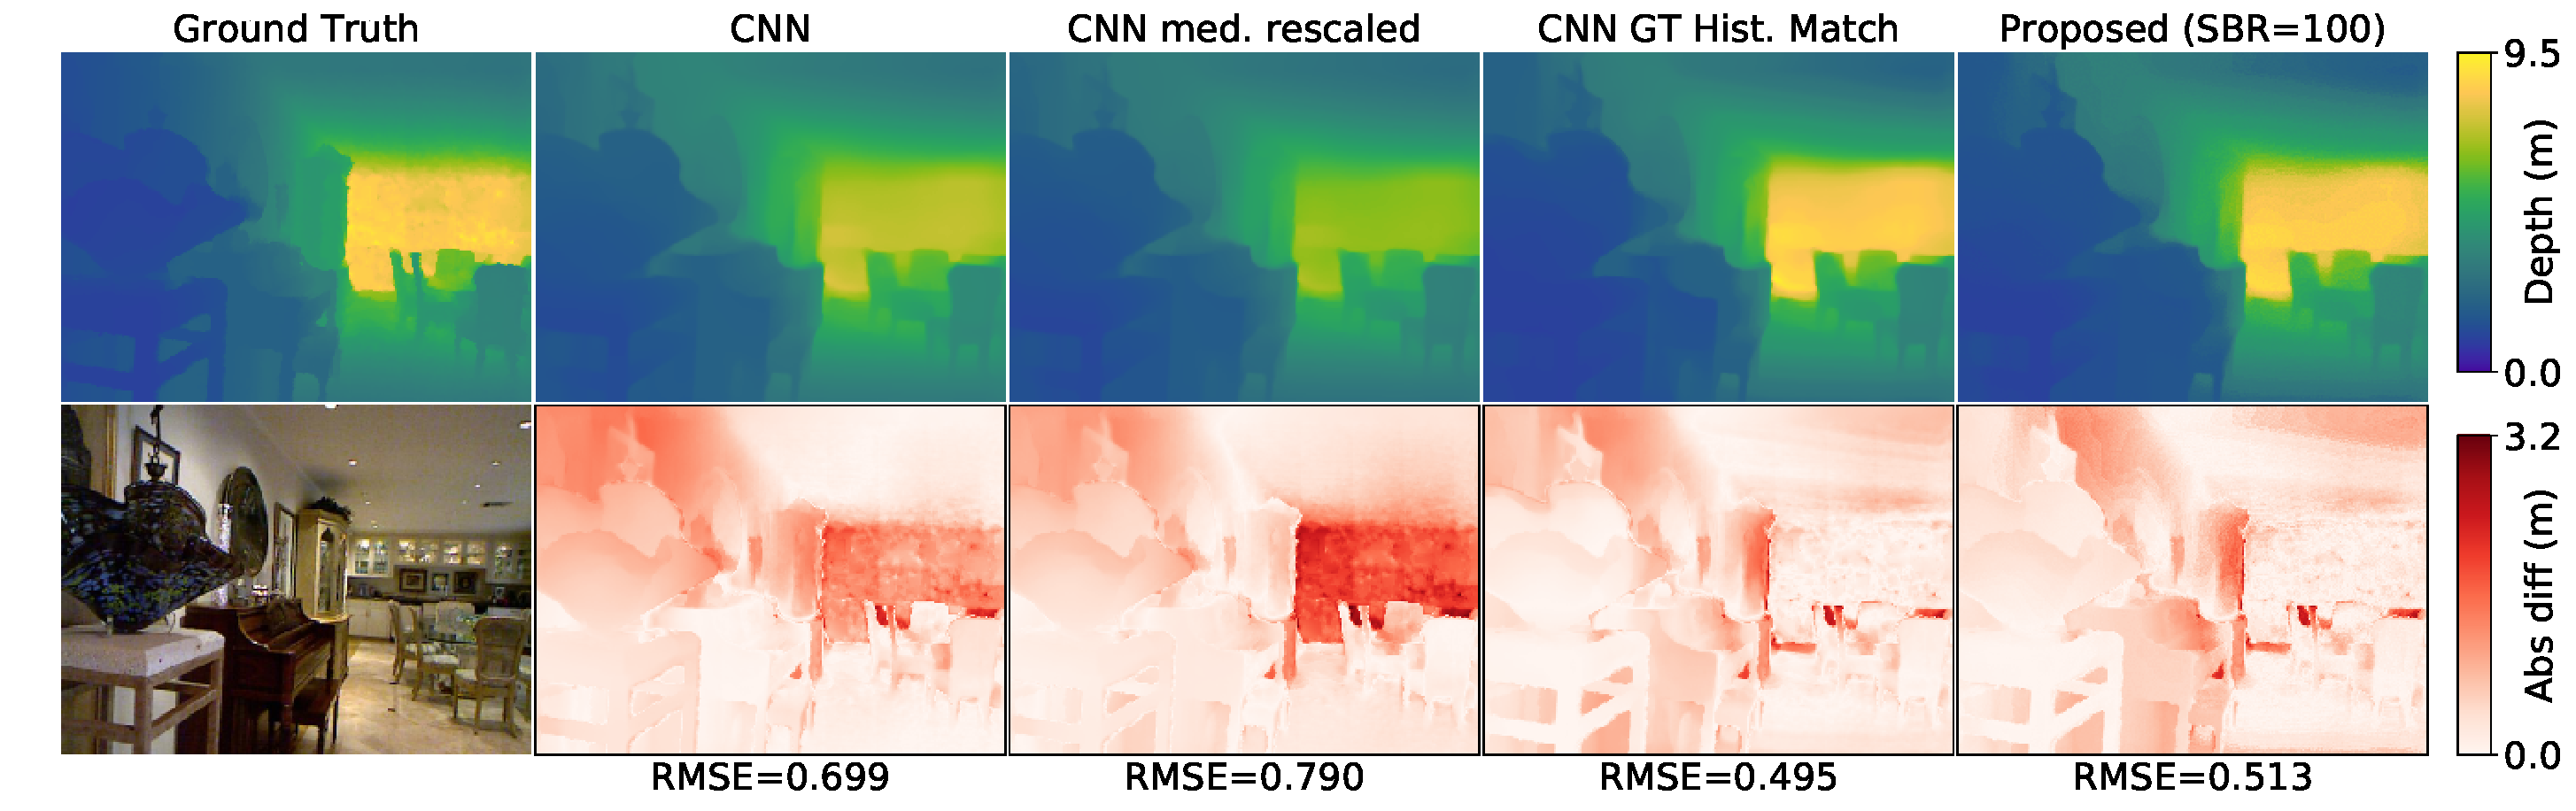
\includegraphics[width=\textwidth]{comparison/densedepth_616_comparison.pdf}
%   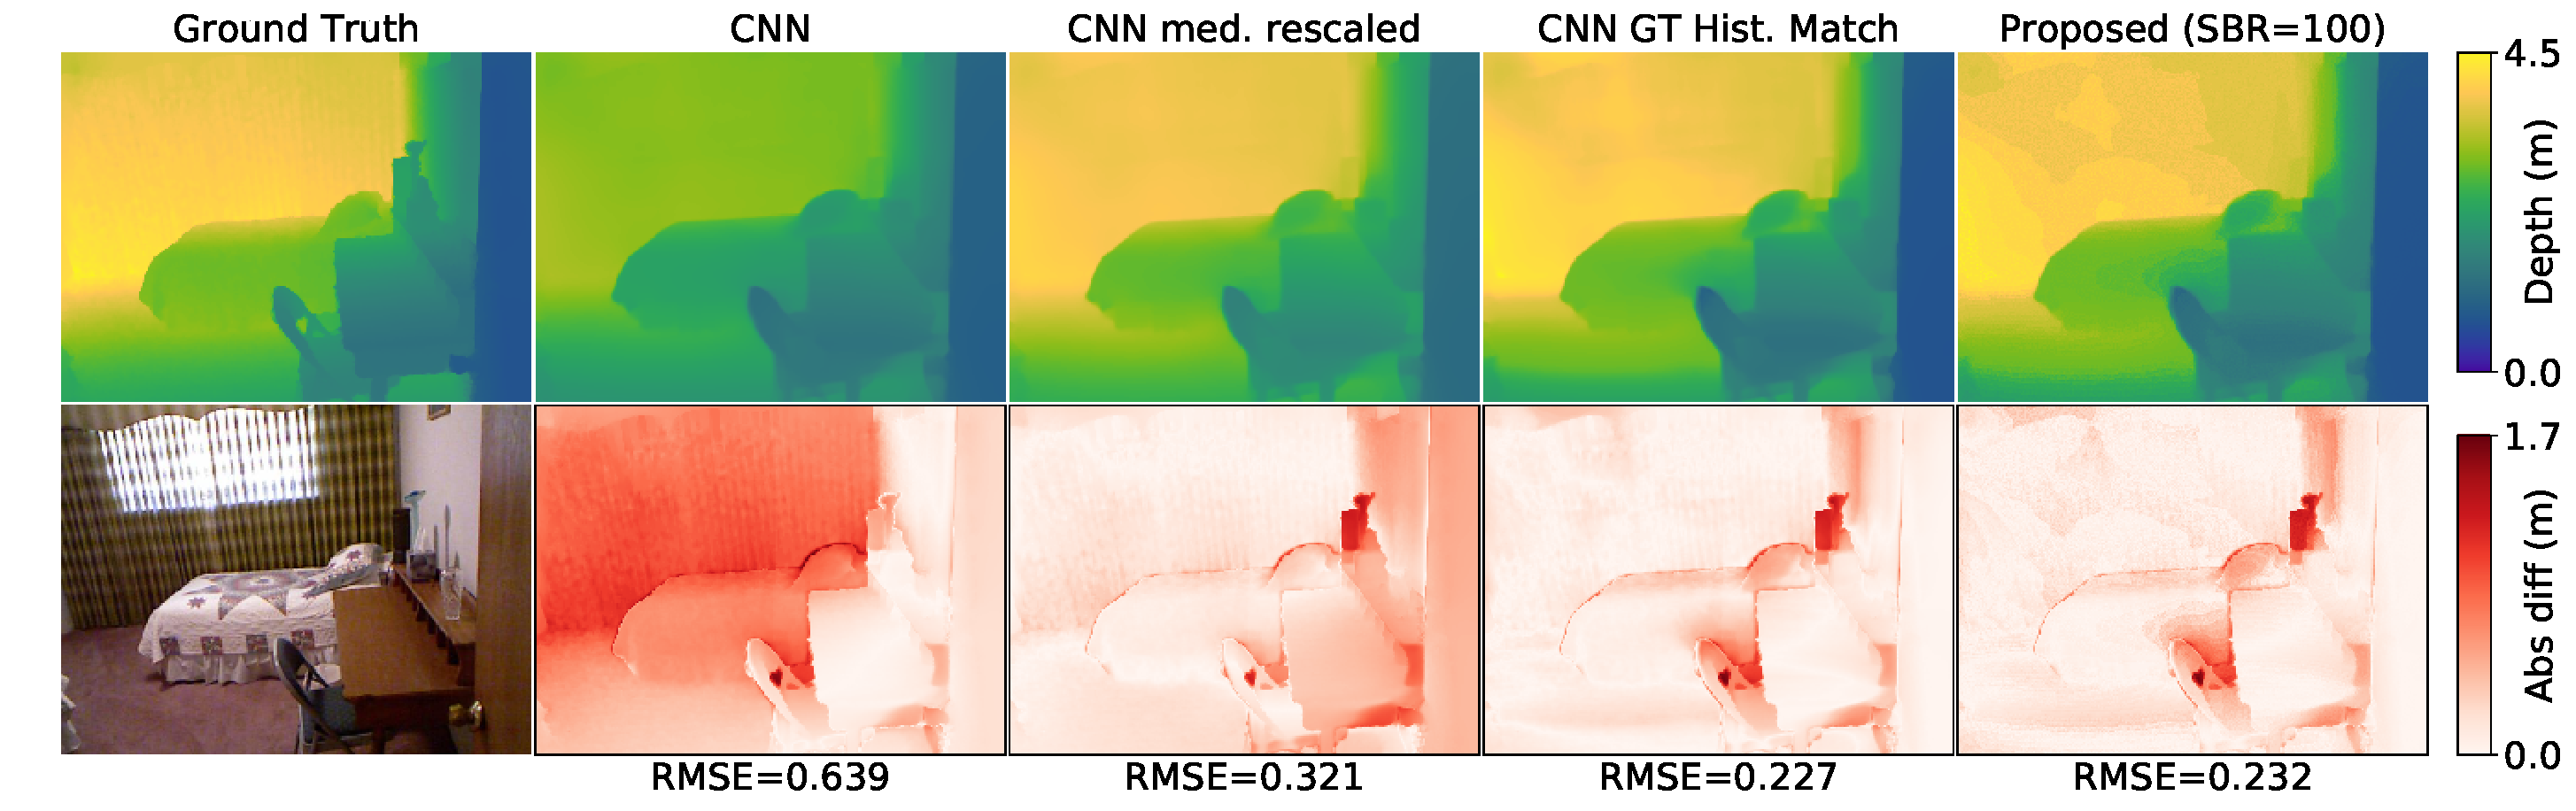
\includegraphics[width=\textwidth]{comparison/densedepth_390_comparison.pdf}
%   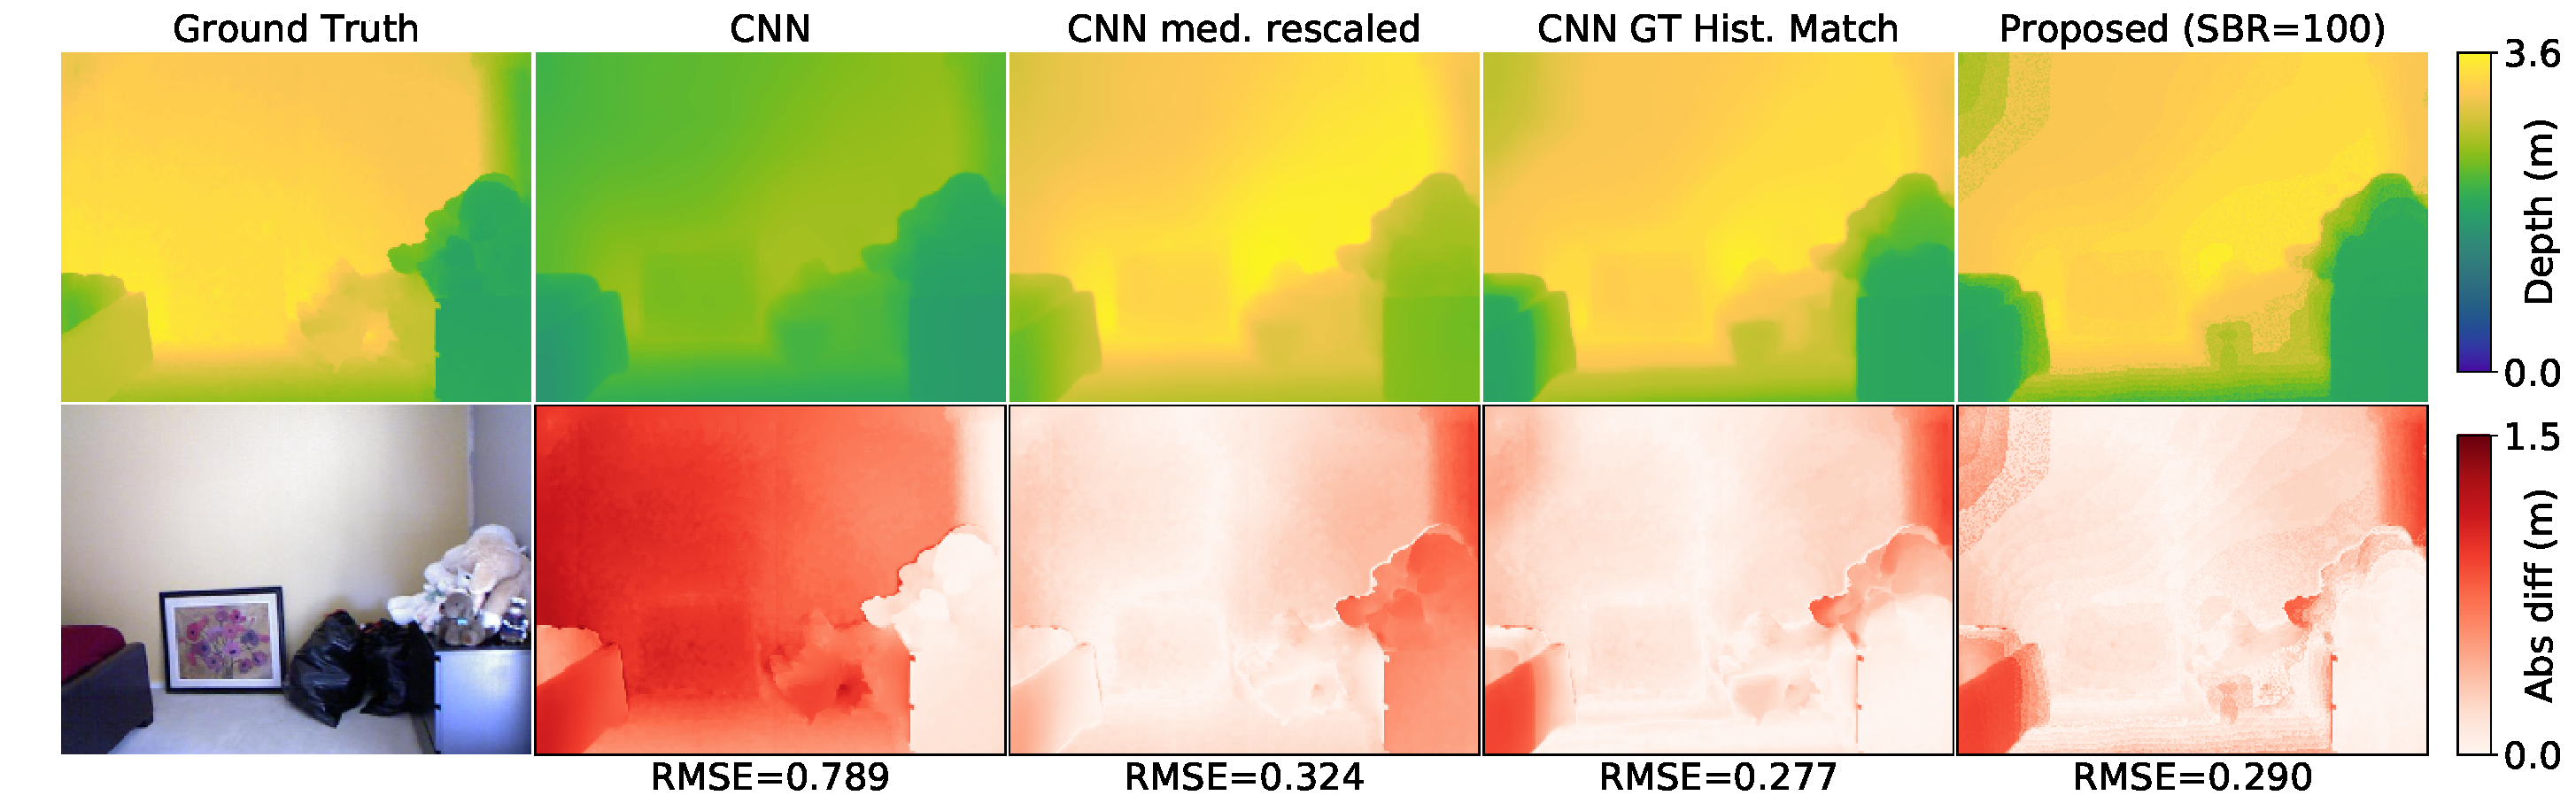
\includegraphics[width=\textwidth]{comparison/densedepth_412_comparison.pdf}
%   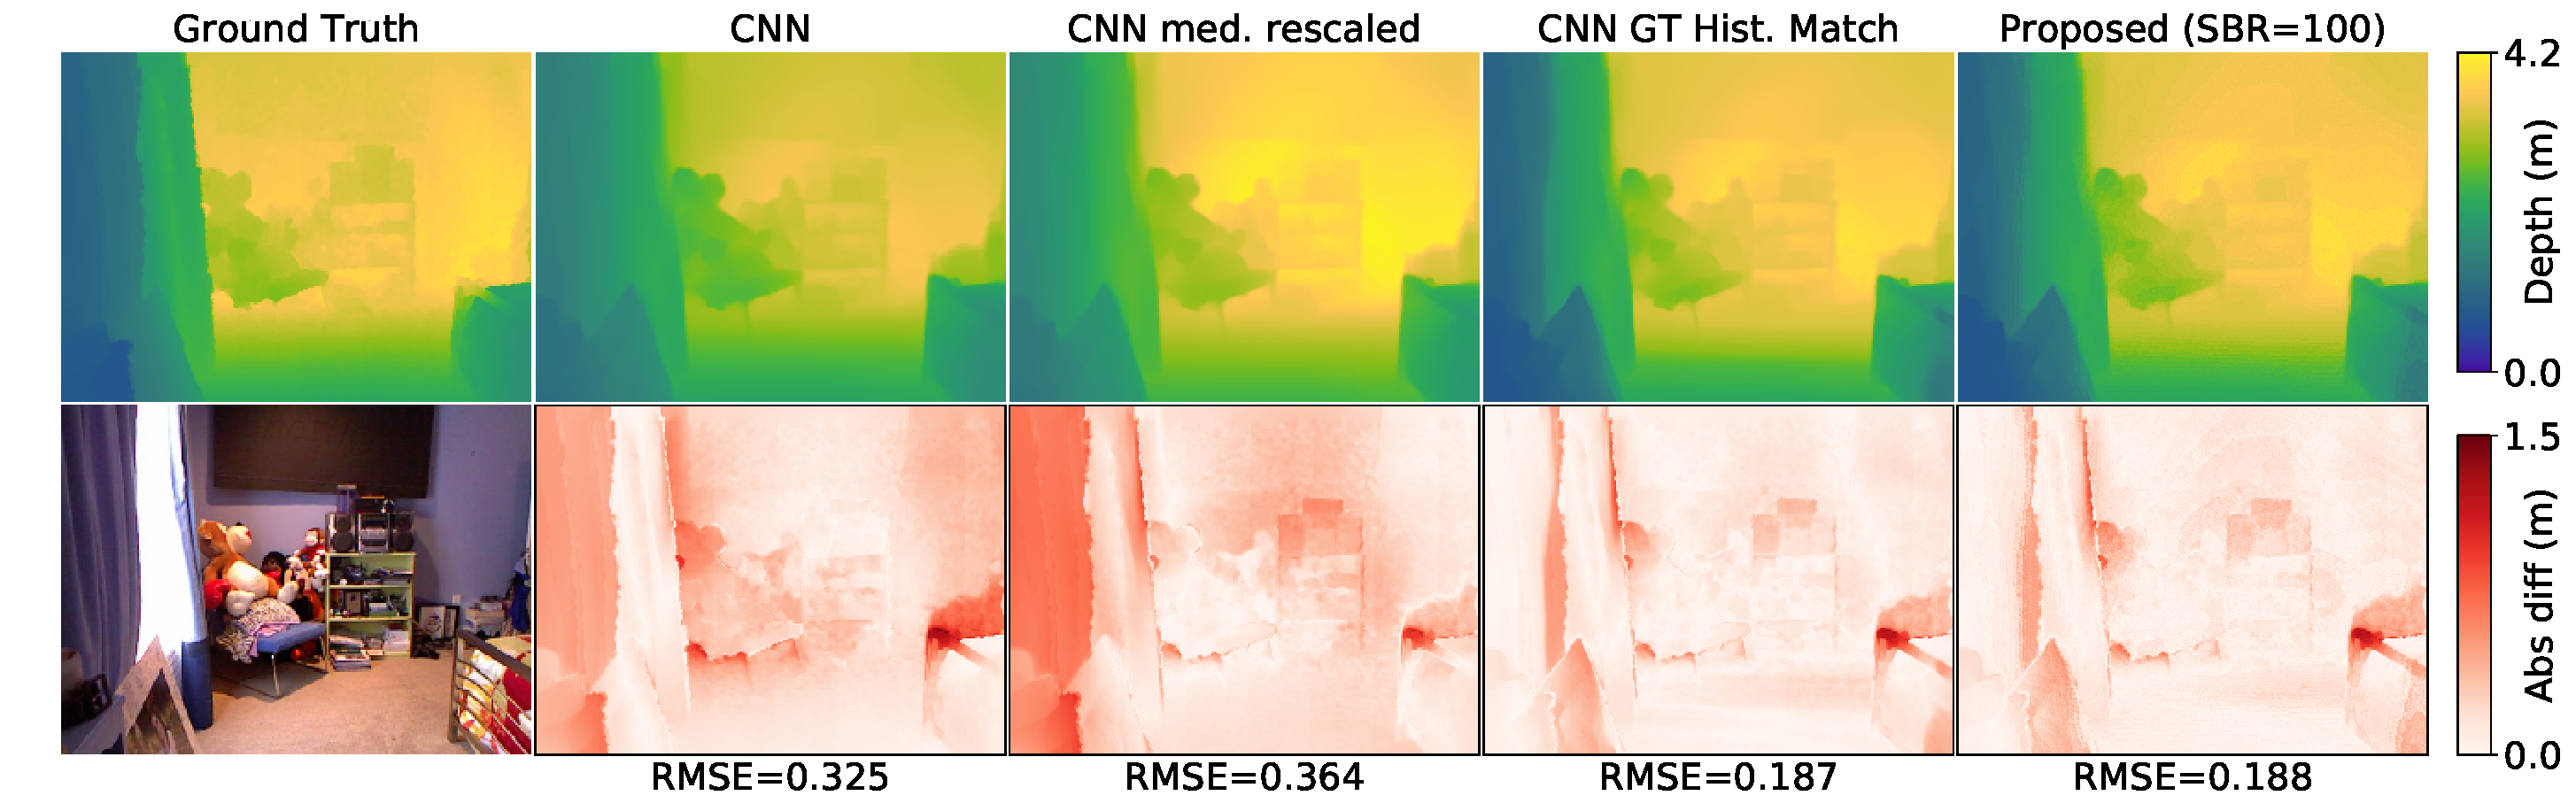
\includegraphics[width=\textwidth]{comparison/densedepth_420_comparison.pdf}
%   \caption{Results on DenseDepth}
% \end{figure}
% \begin{figure}
%   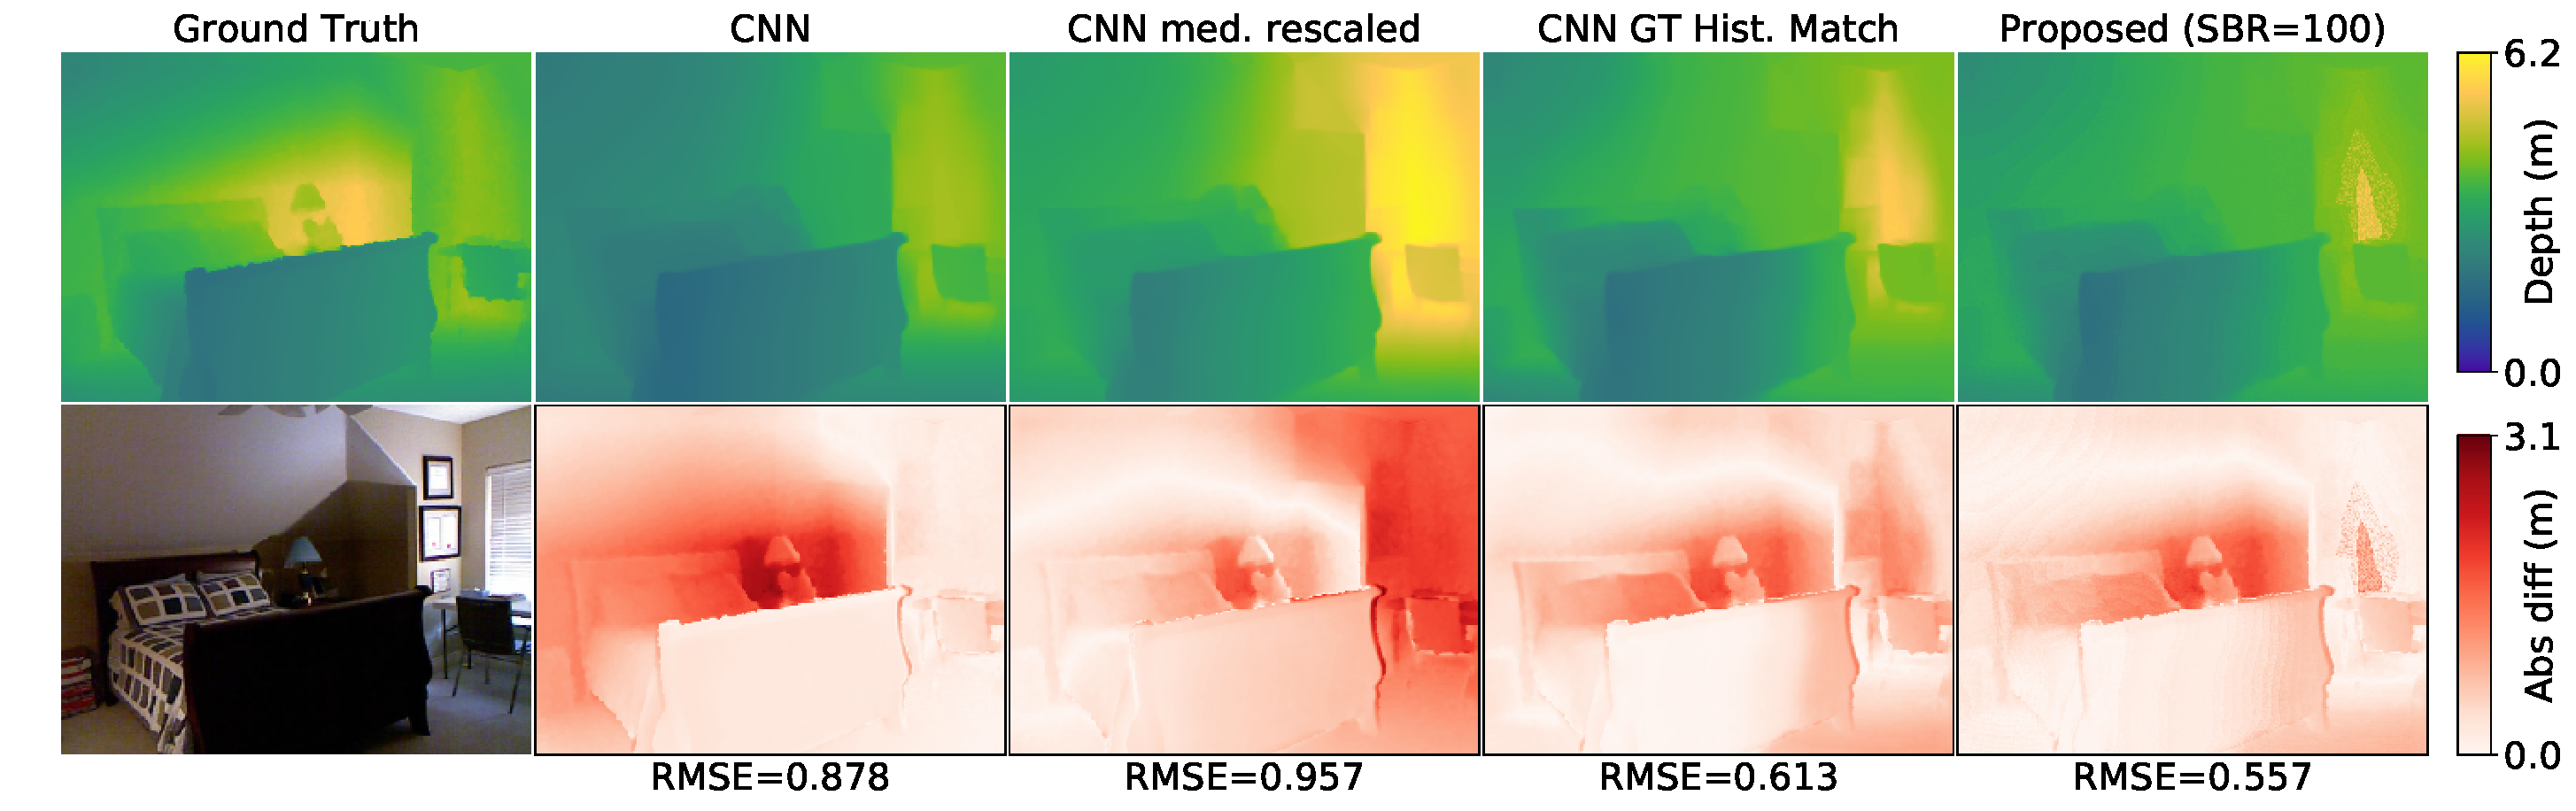
\includegraphics[width=\textwidth]{comparison/densedepth_428_comparison.pdf}
%   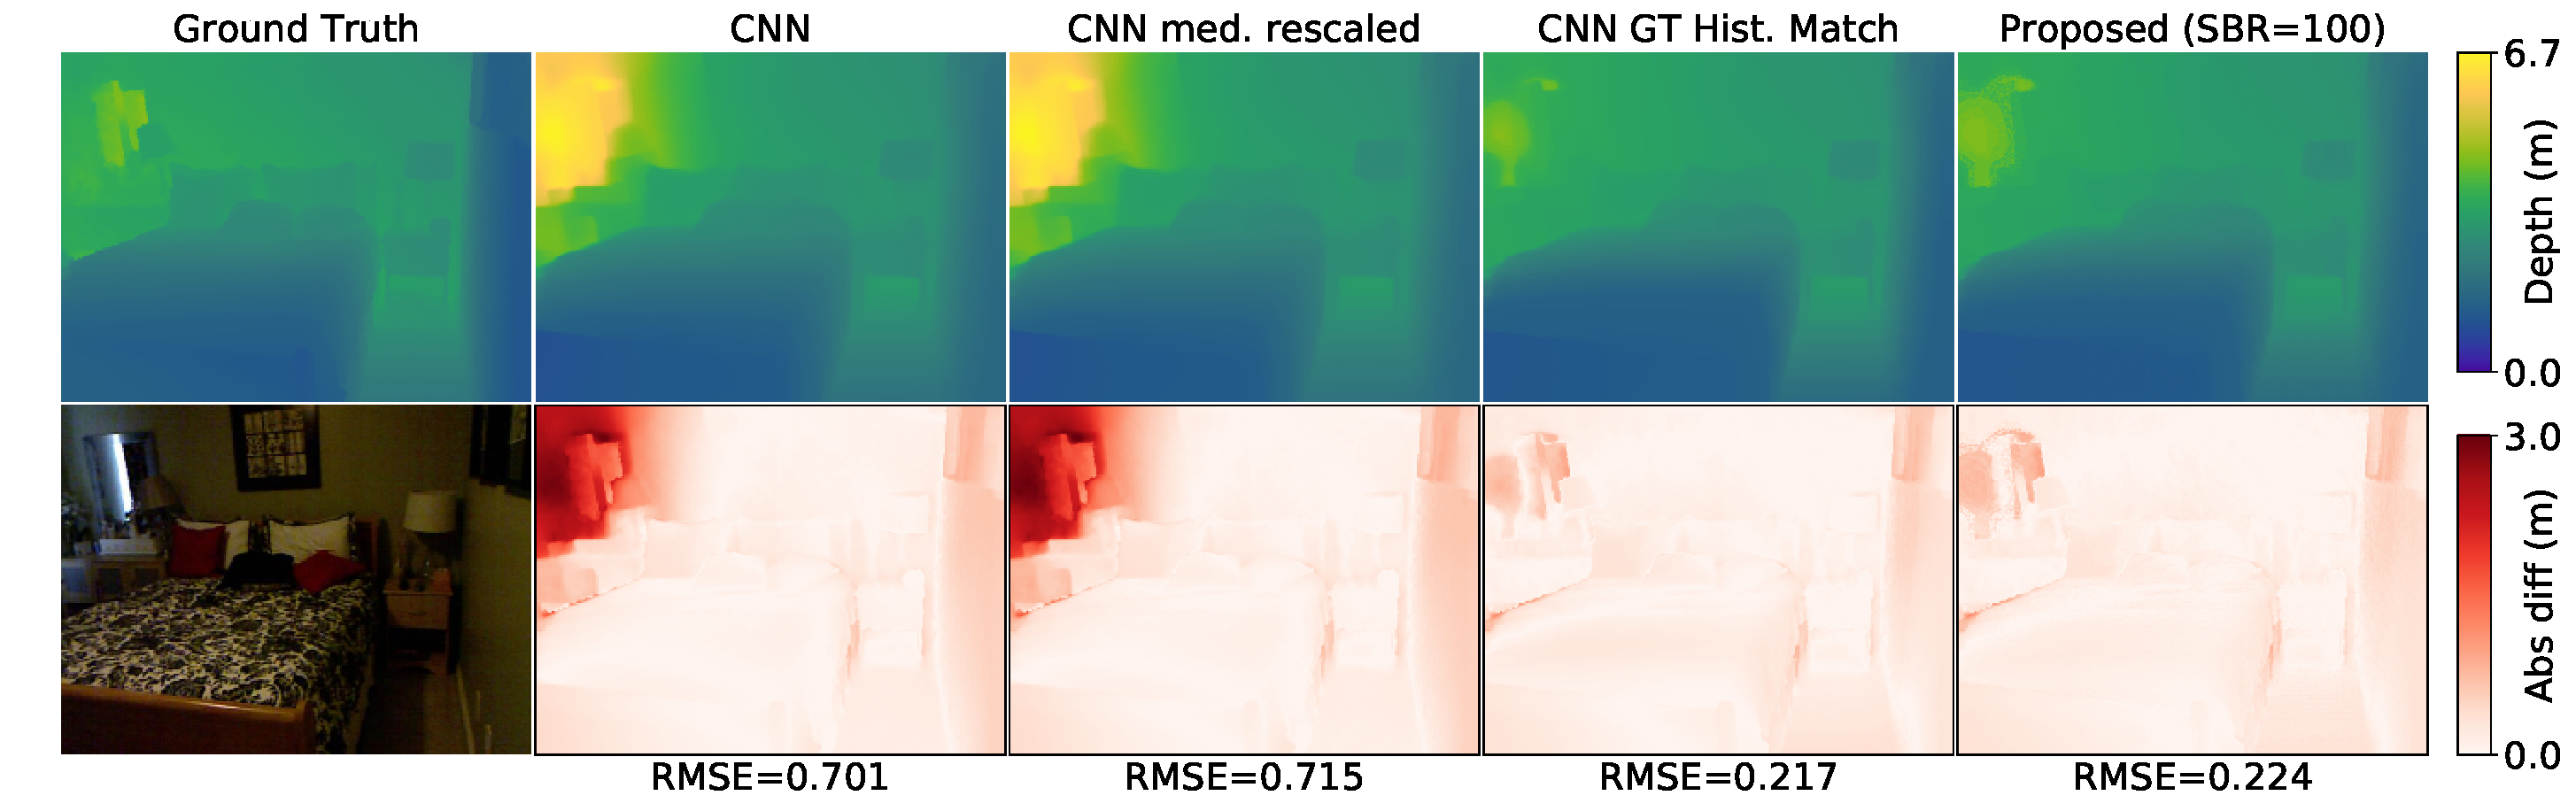
\includegraphics[width=\textwidth]{comparison/densedepth_457_comparison.pdf}
%   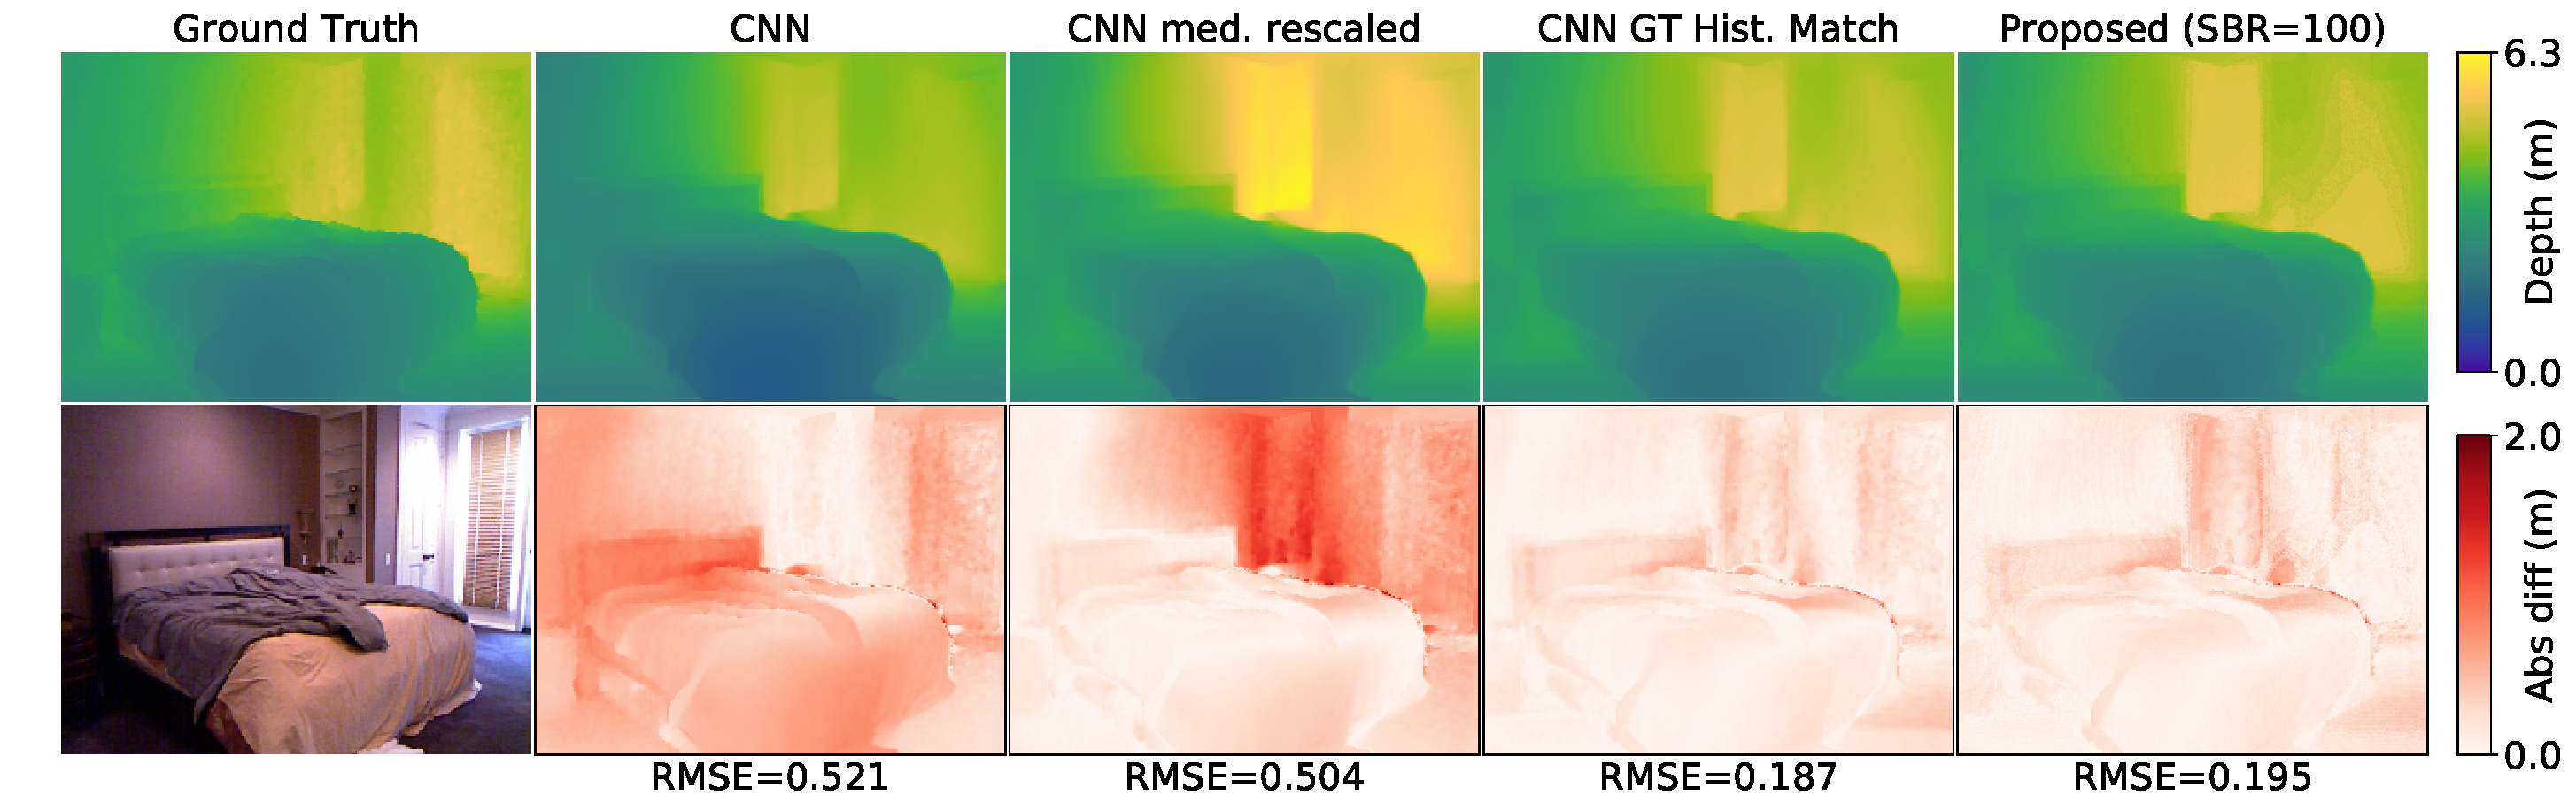
\includegraphics[width=\textwidth]{comparison/densedepth_468_comparison.pdf}
%   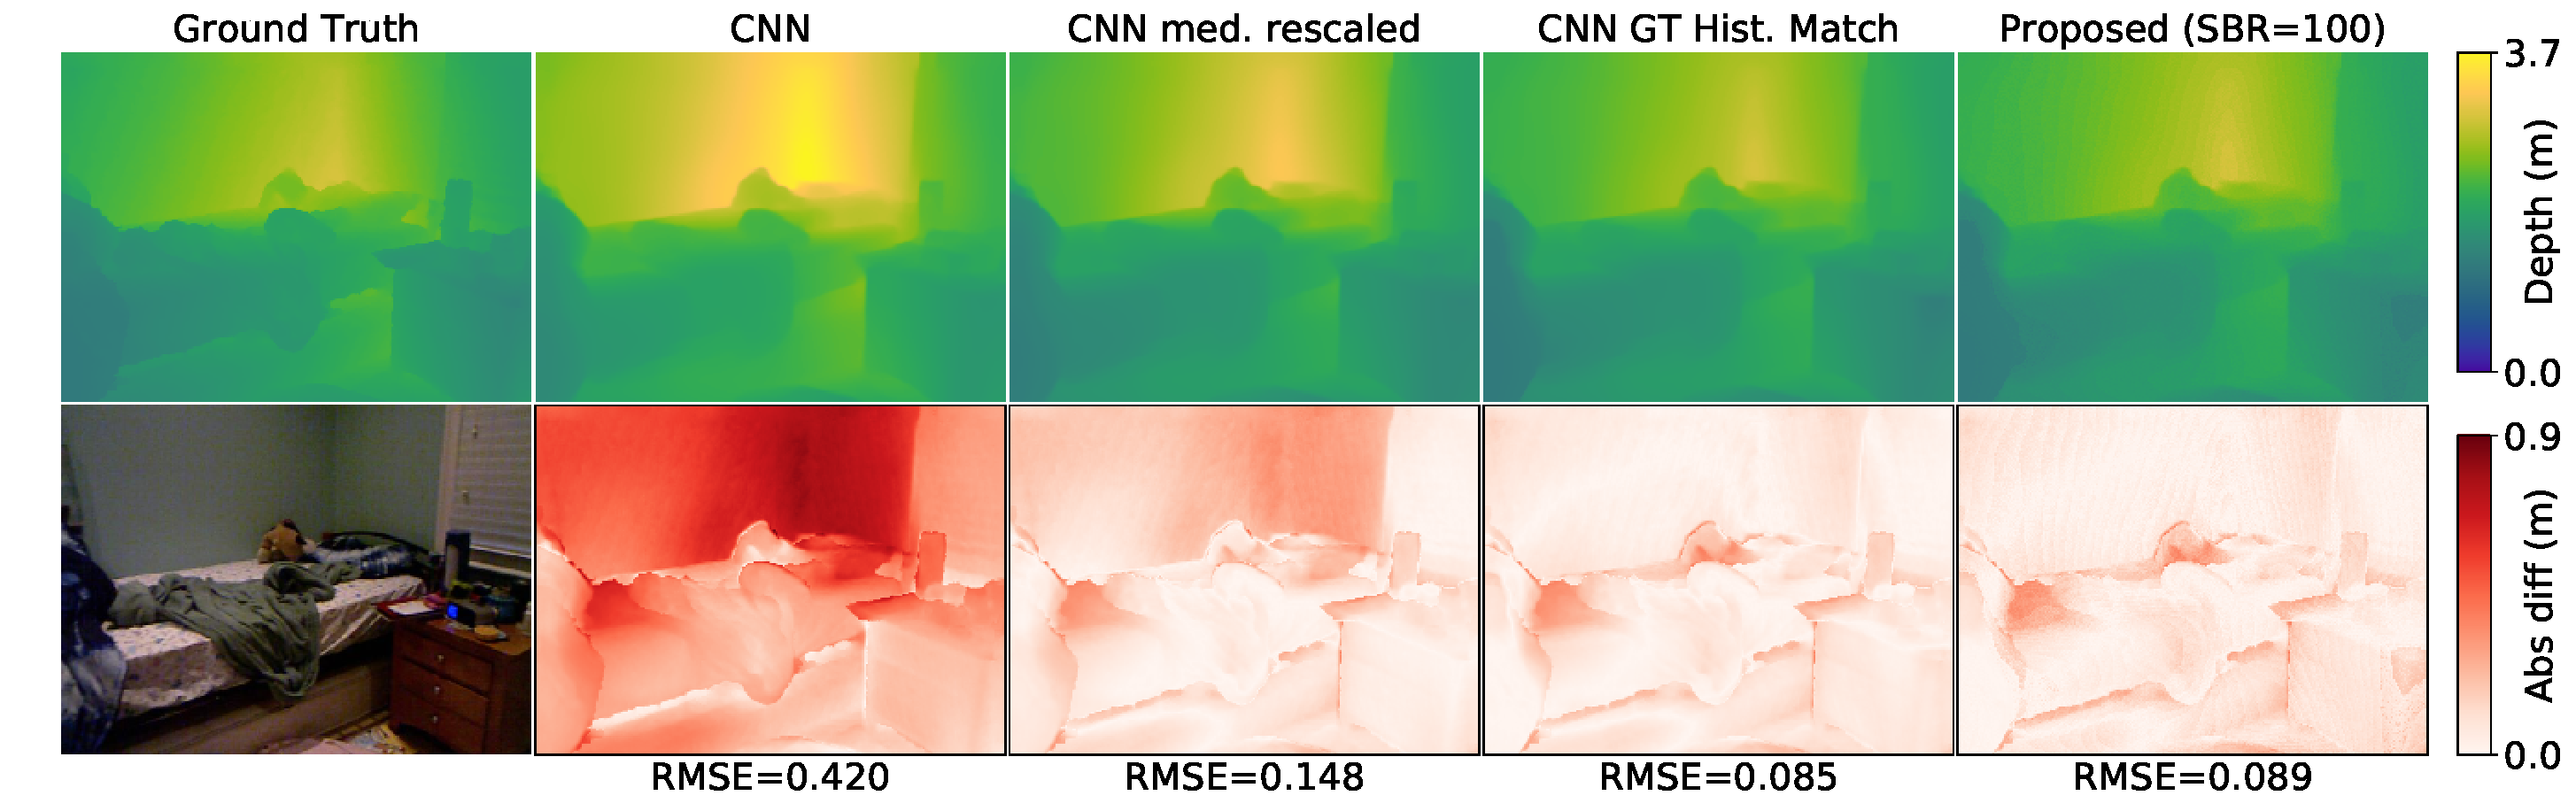
\includegraphics[width=\textwidth]{comparison/densedepth_477_comparison.pdf}
%   \caption{Results on DenseDepth}
% \end{figure}
%   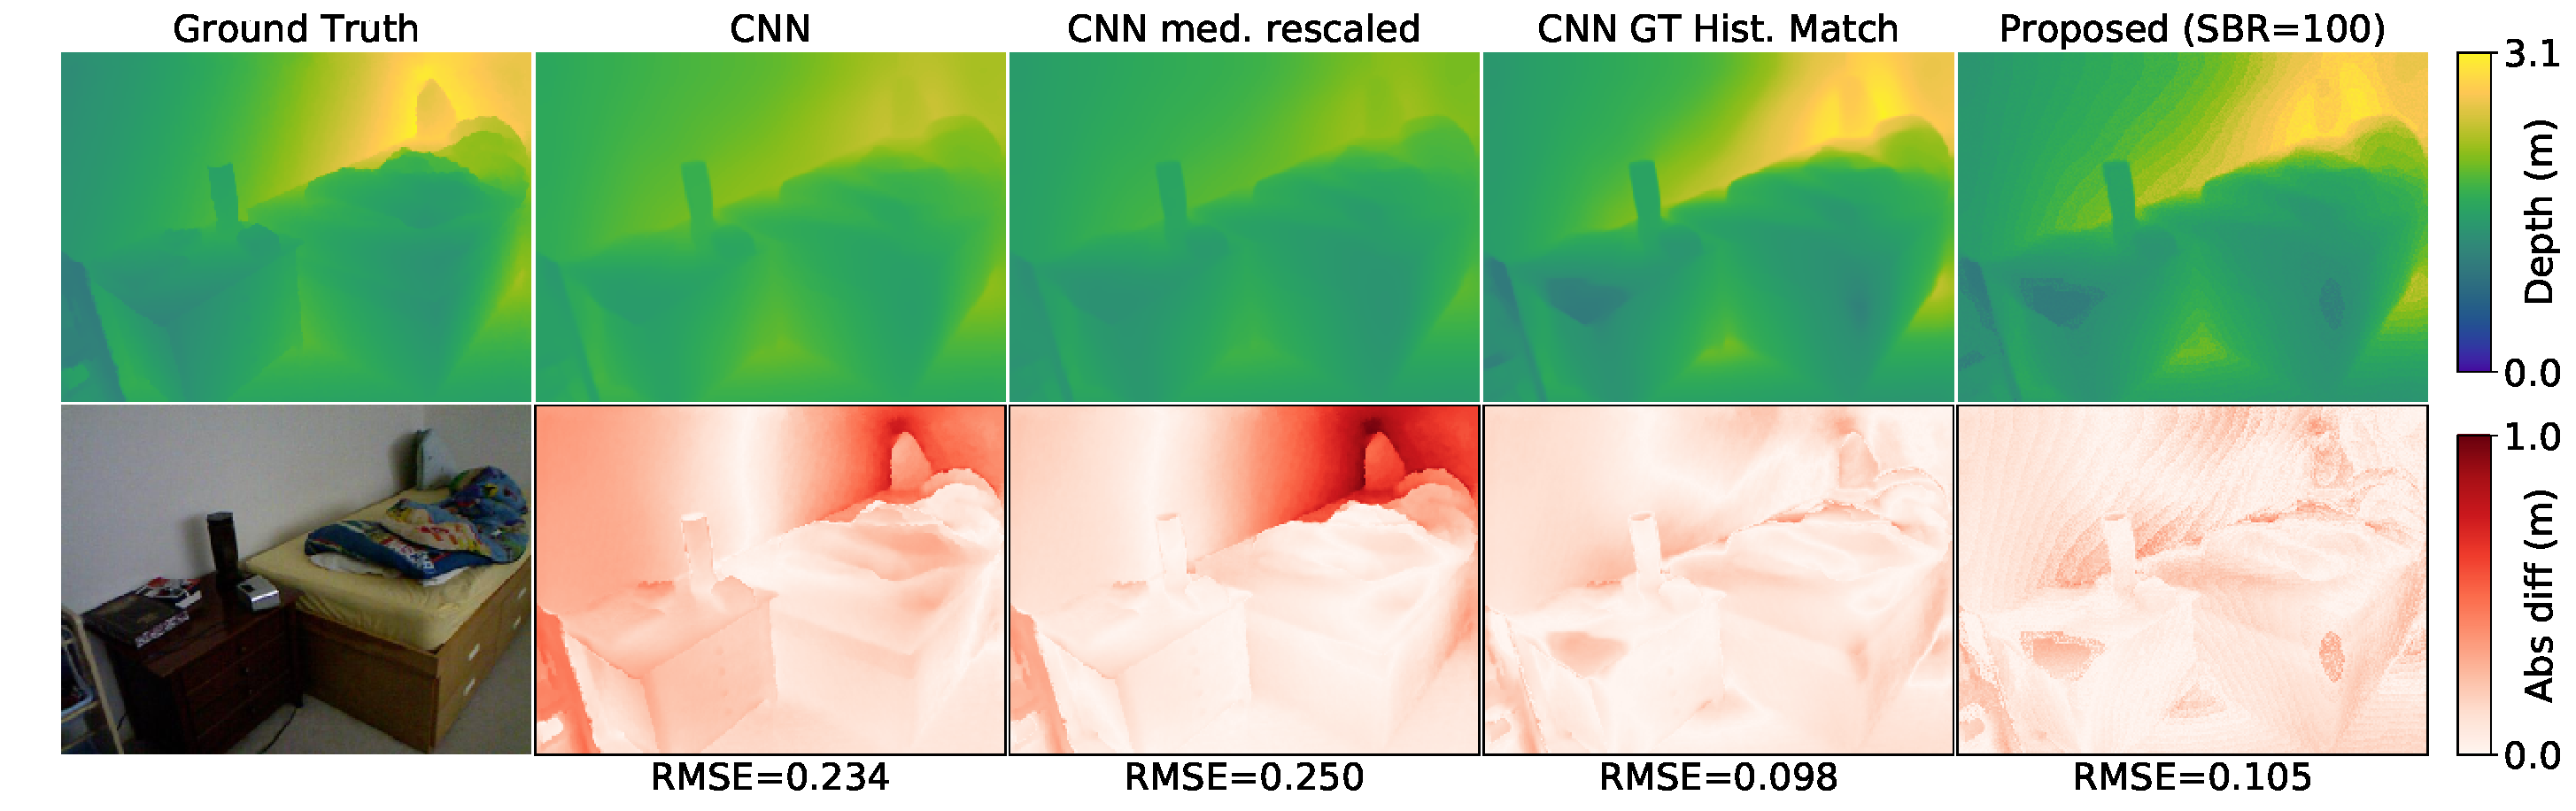
\includegraphics[height=3cm]{comparison/densedepth_499_comparison.pdf}
%   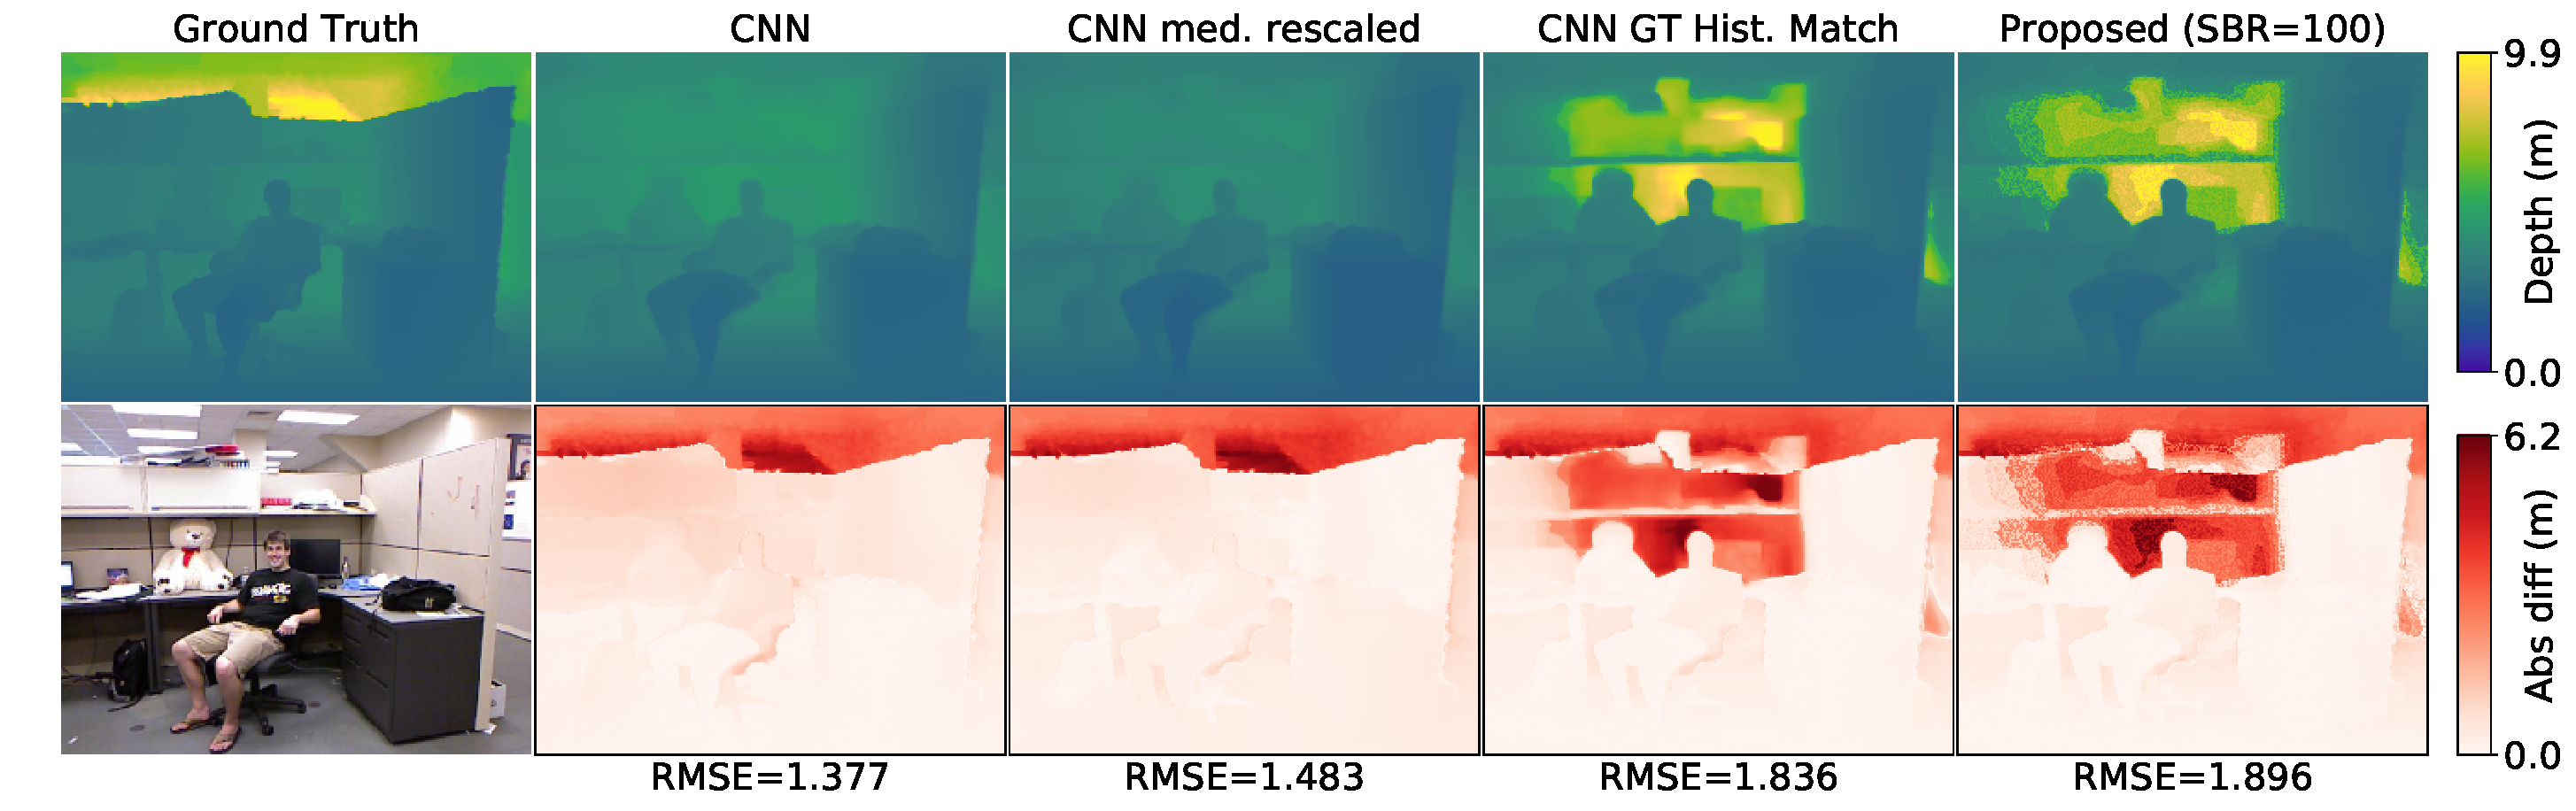
\includegraphics[height=3cm]{comparison/densedepth_258_comparison.pdf}
%   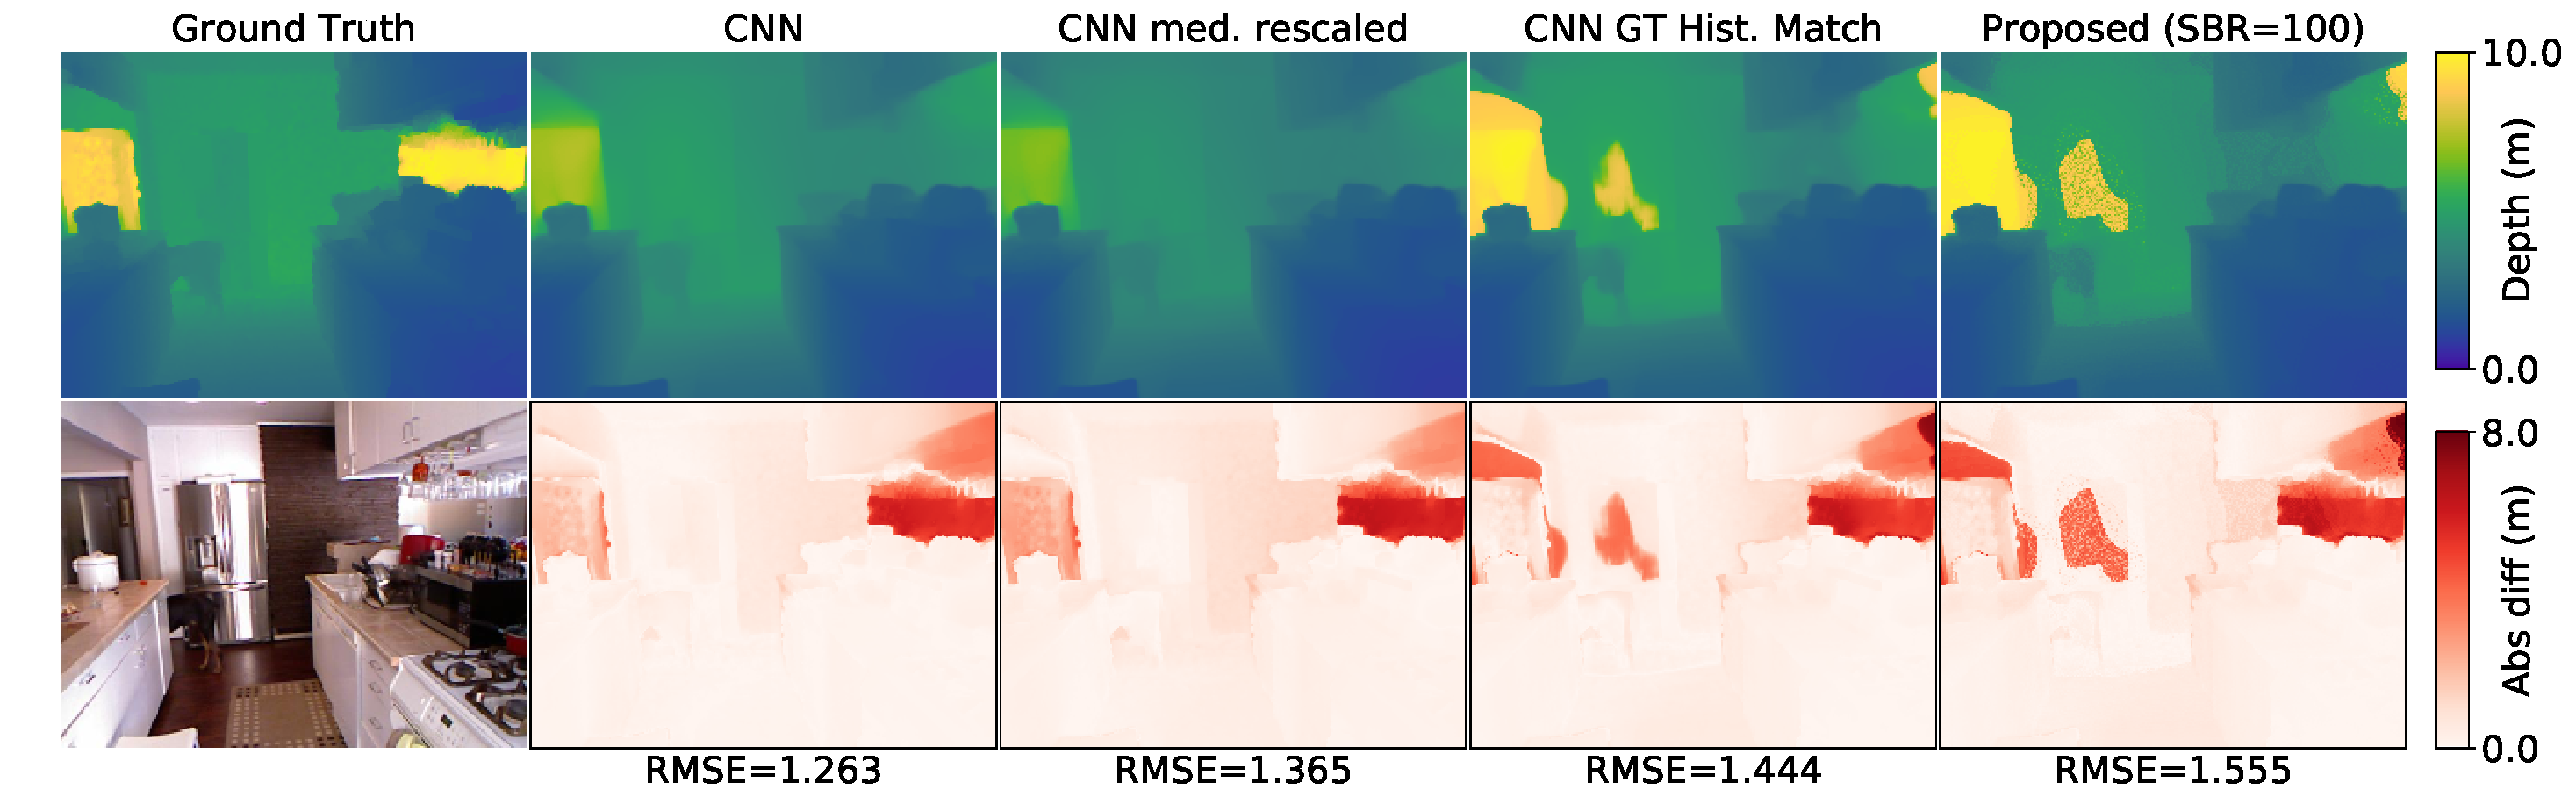
\includegraphics[height=3cm]{comparison/densedepth_341_comparison.pdf}
\begin{figure}[H]
  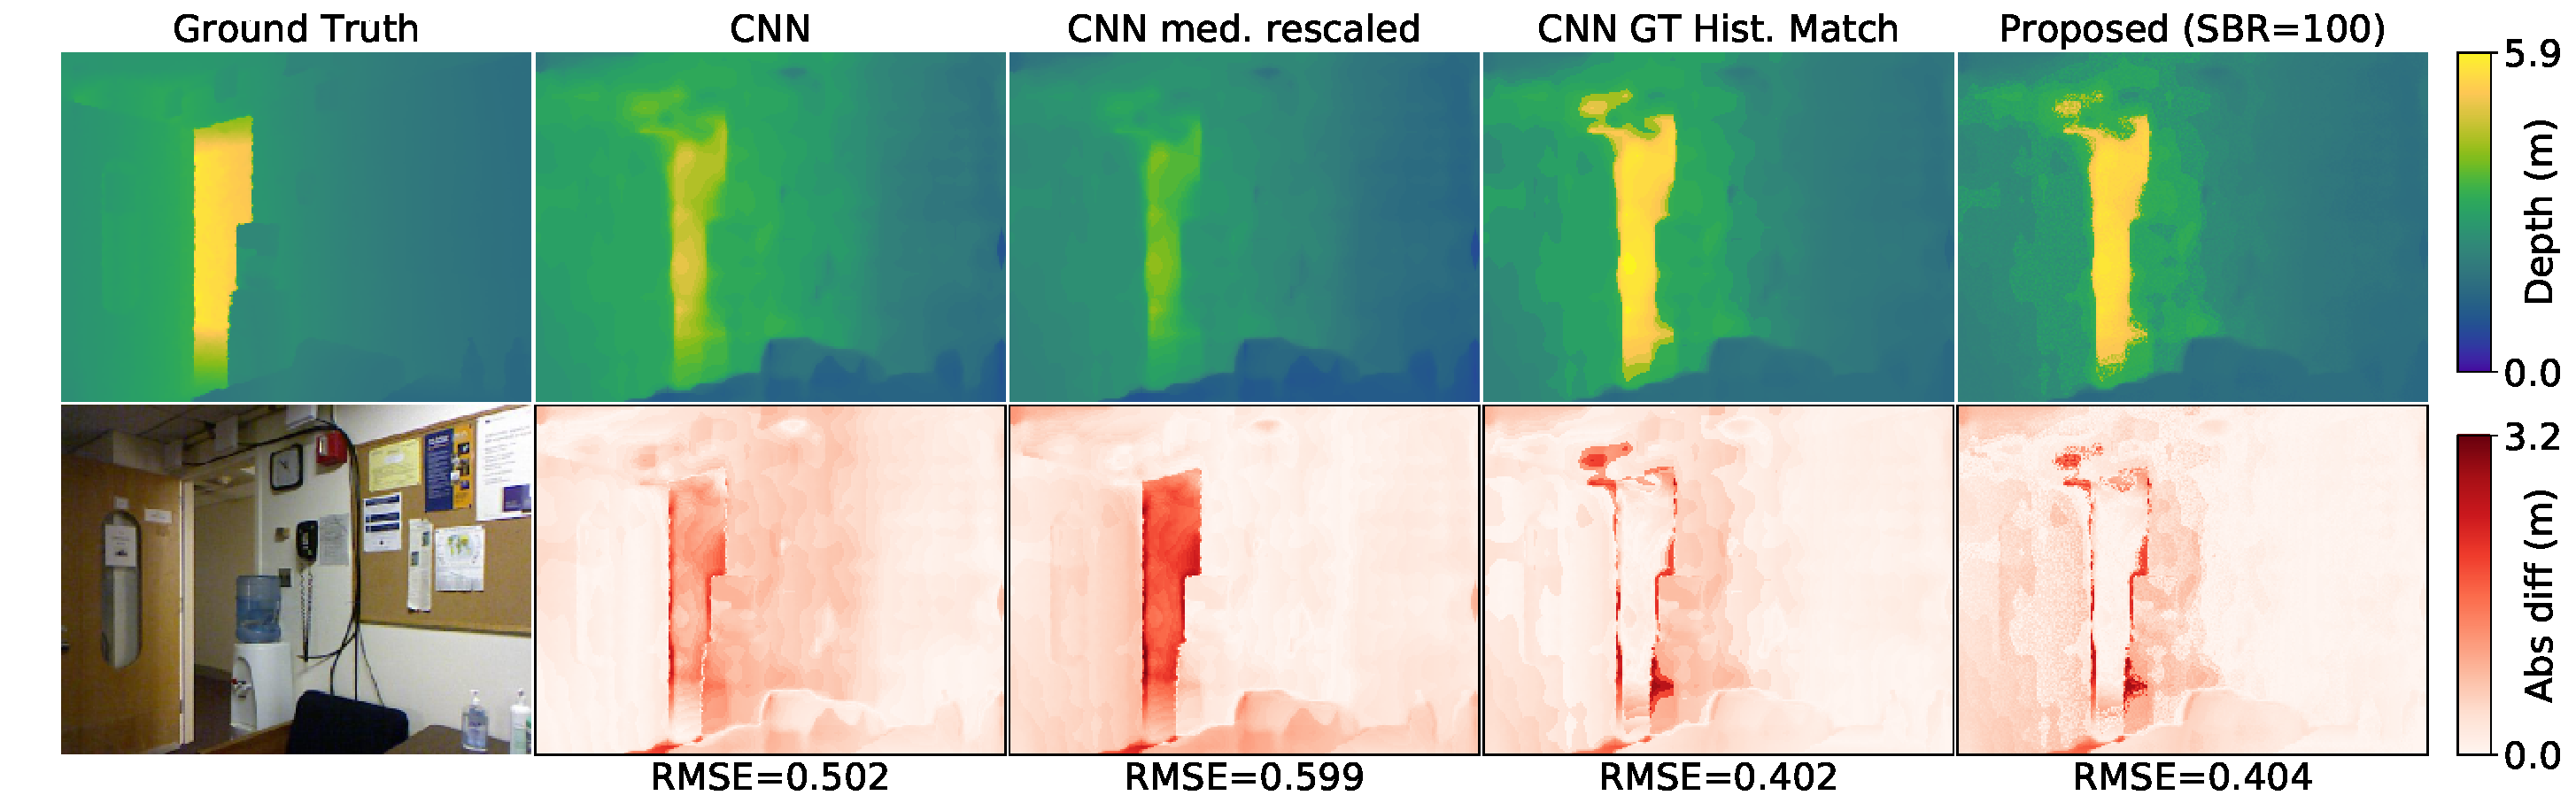
\includegraphics[width=\textwidth]{comparison/dorn_8_comparison.pdf}
  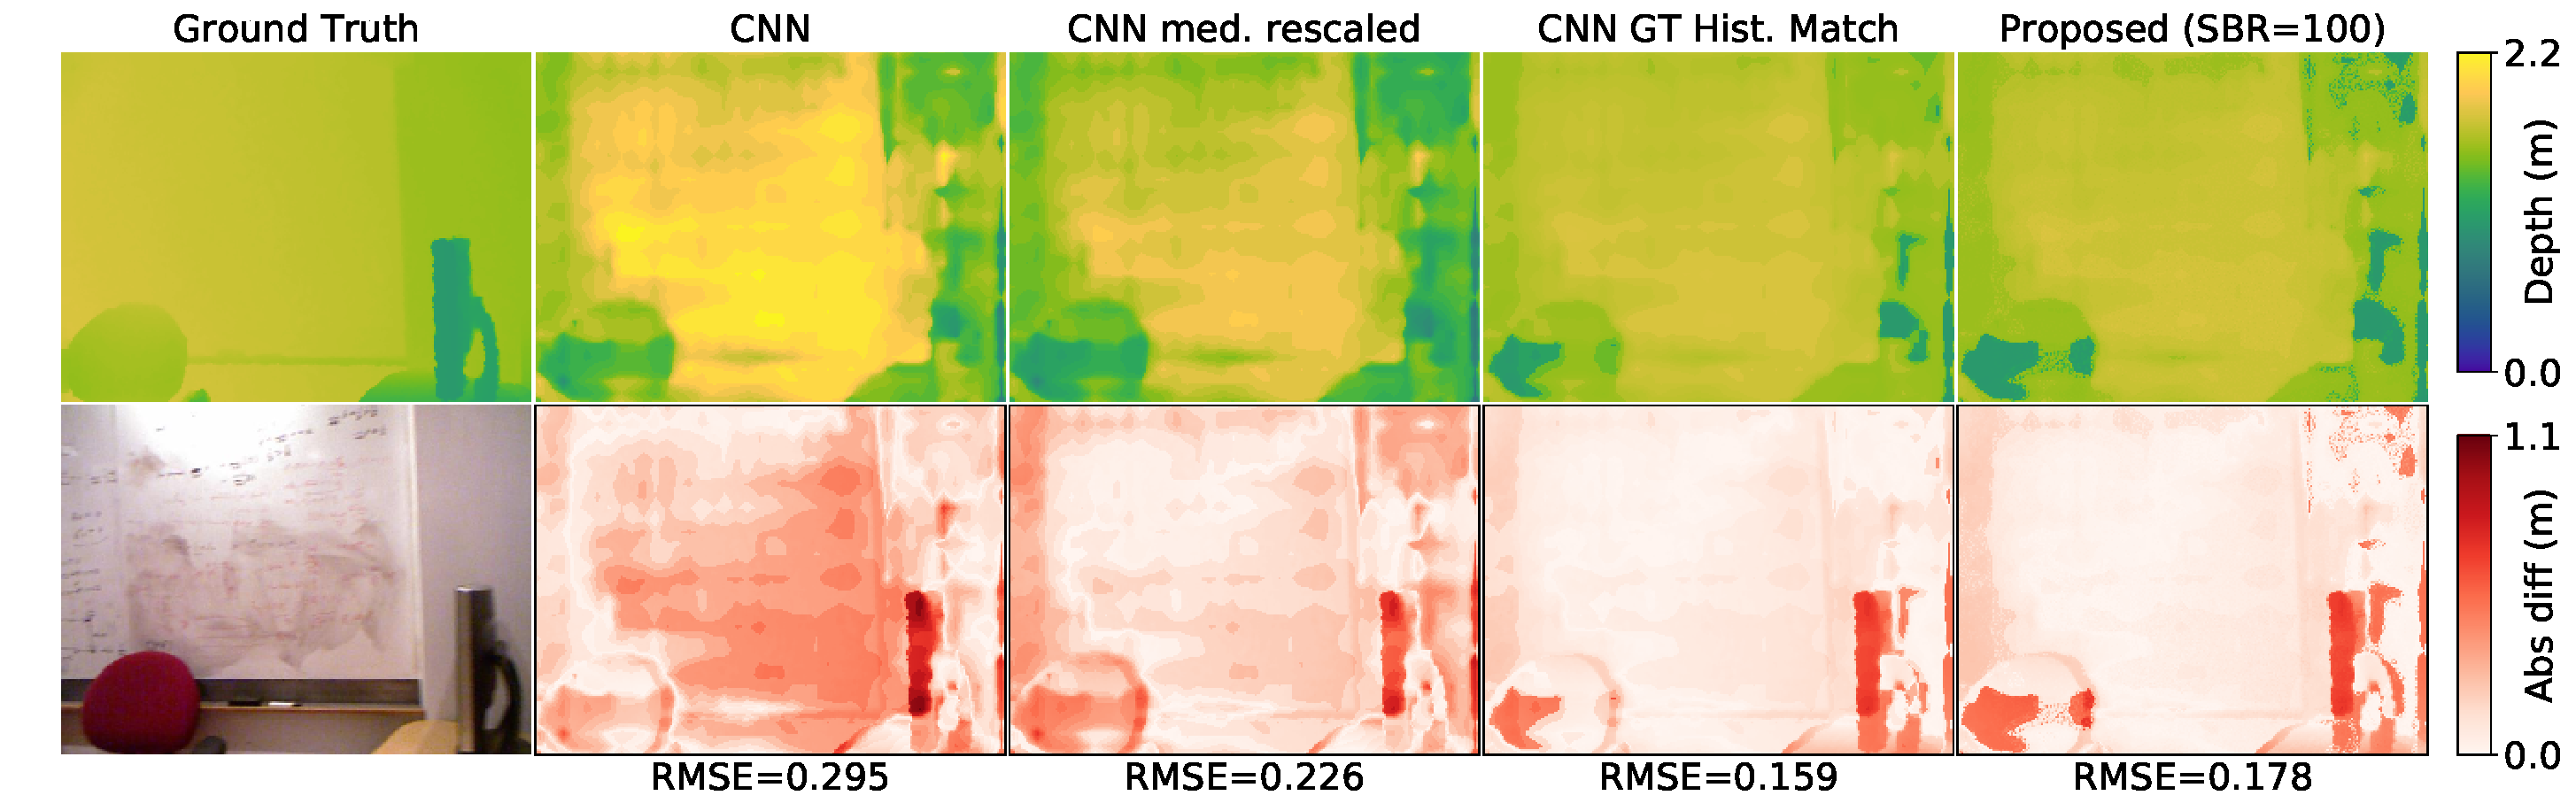
\includegraphics[width=\textwidth]{comparison/dorn_14_comparison.pdf}
  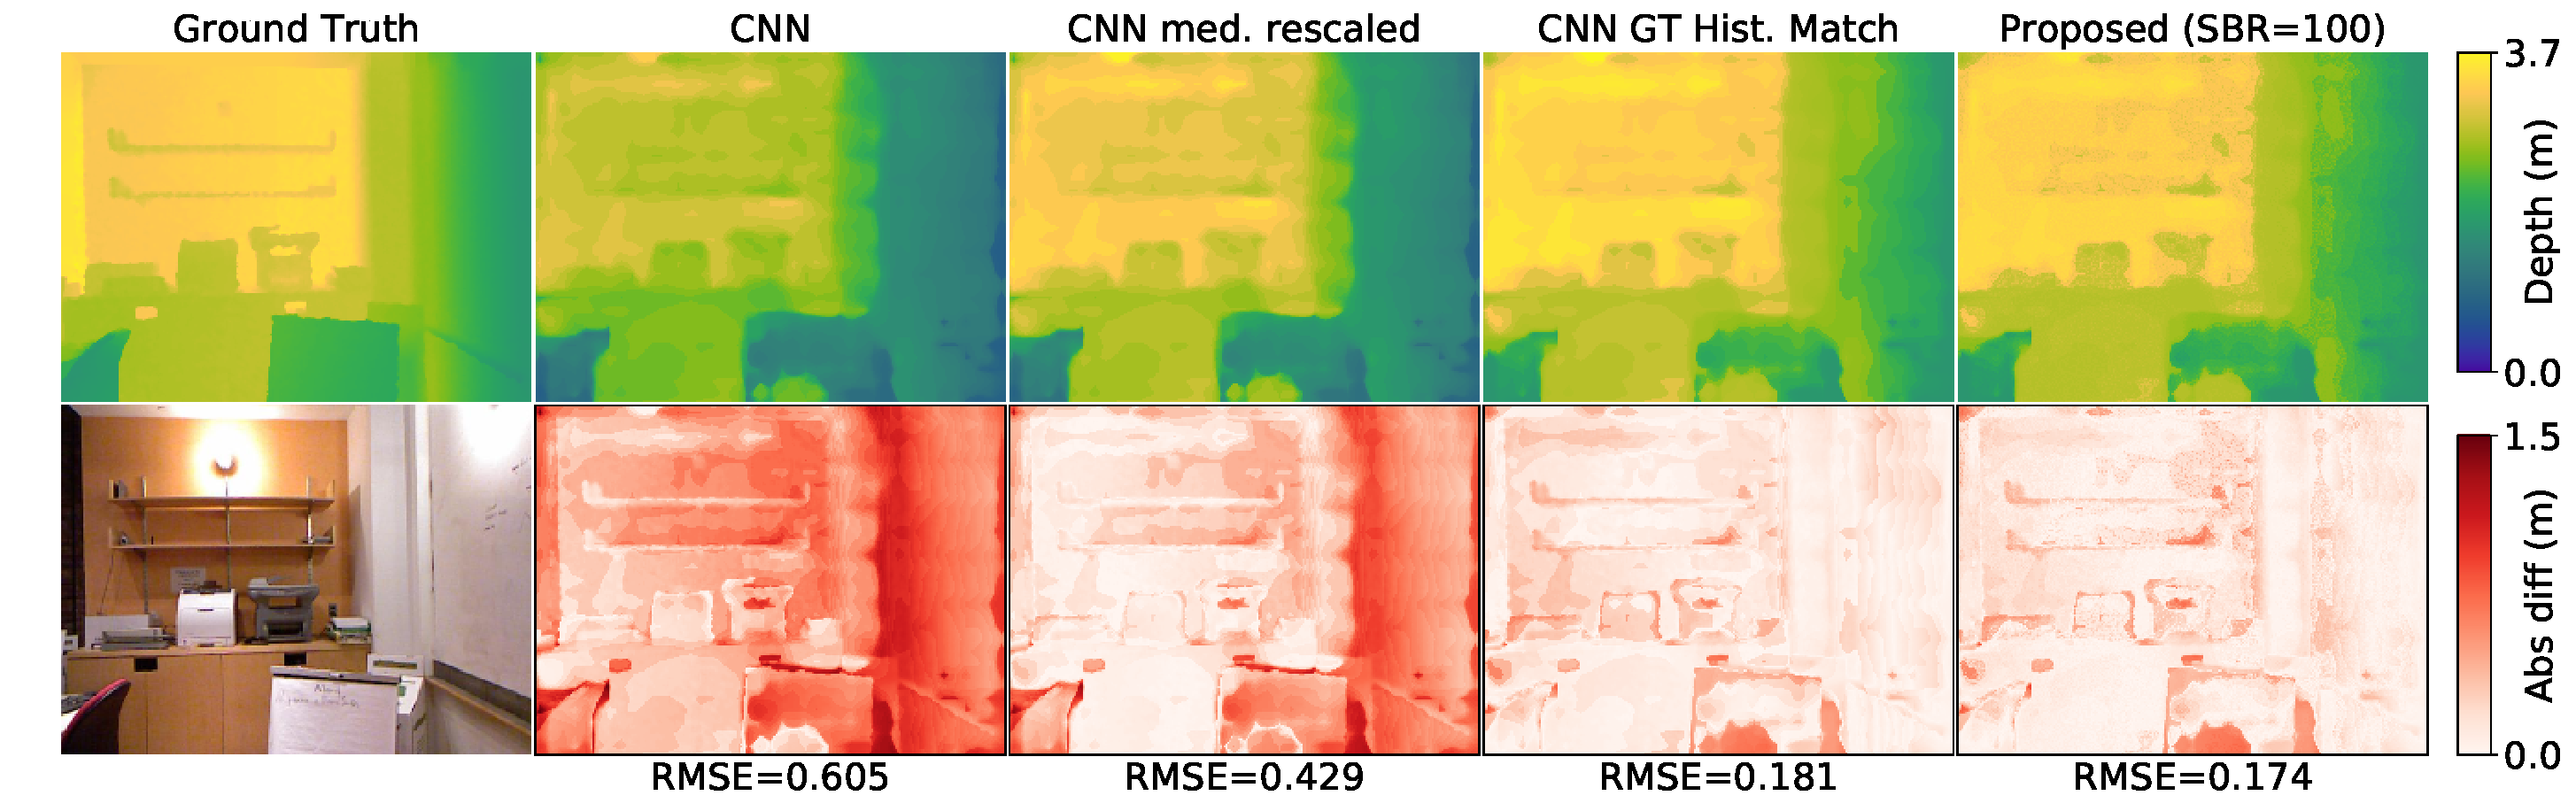
\includegraphics[width=\textwidth]{comparison/dorn_15_comparison.pdf}
  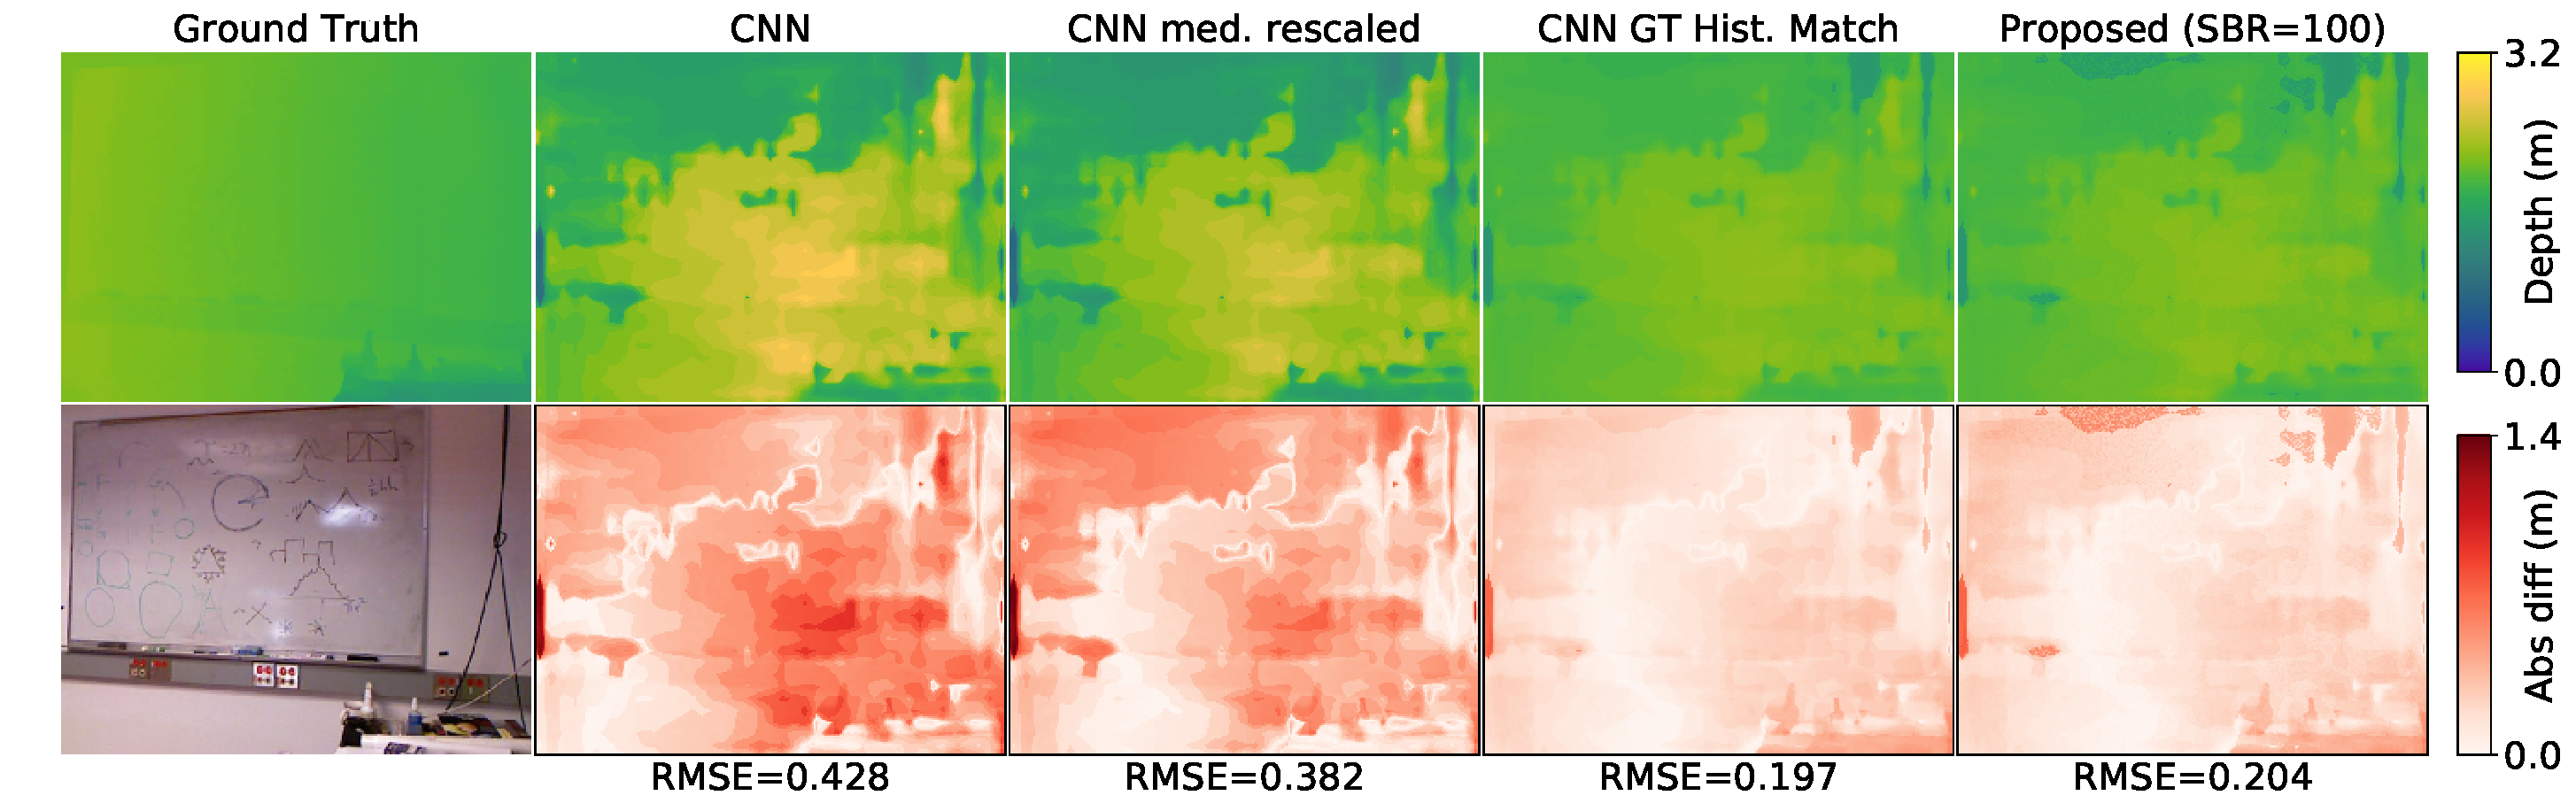
\includegraphics[width=\textwidth]{comparison/dorn_23_comparison.pdf}
  \caption{Results with DORN as the monocular depth estimator. Our method is able to scale and shift
    the depth maps to mitigate gross errors in depth scaling.}
  \label{fig:dorn_1}
\end{figure}
\begin{figure}[H]
  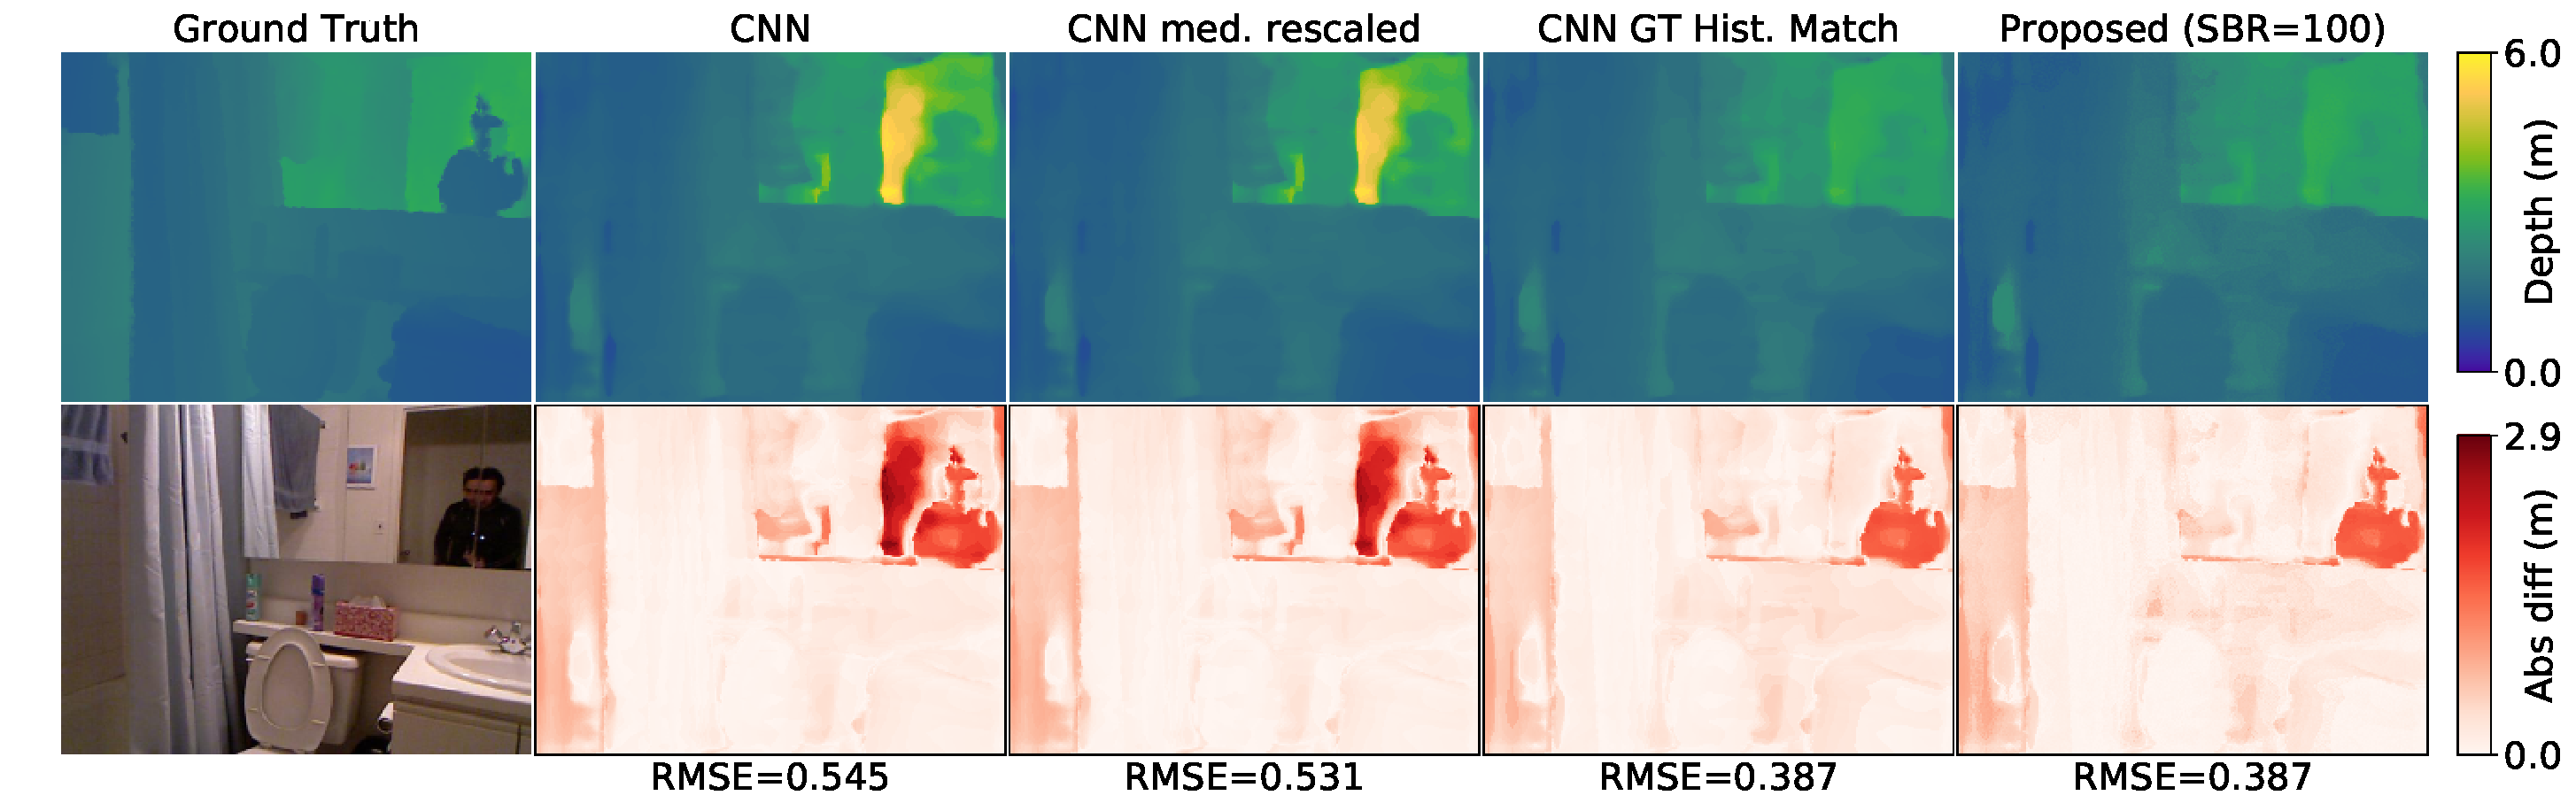
\includegraphics[width=\textwidth]{comparison/dorn_26_comparison.pdf}
  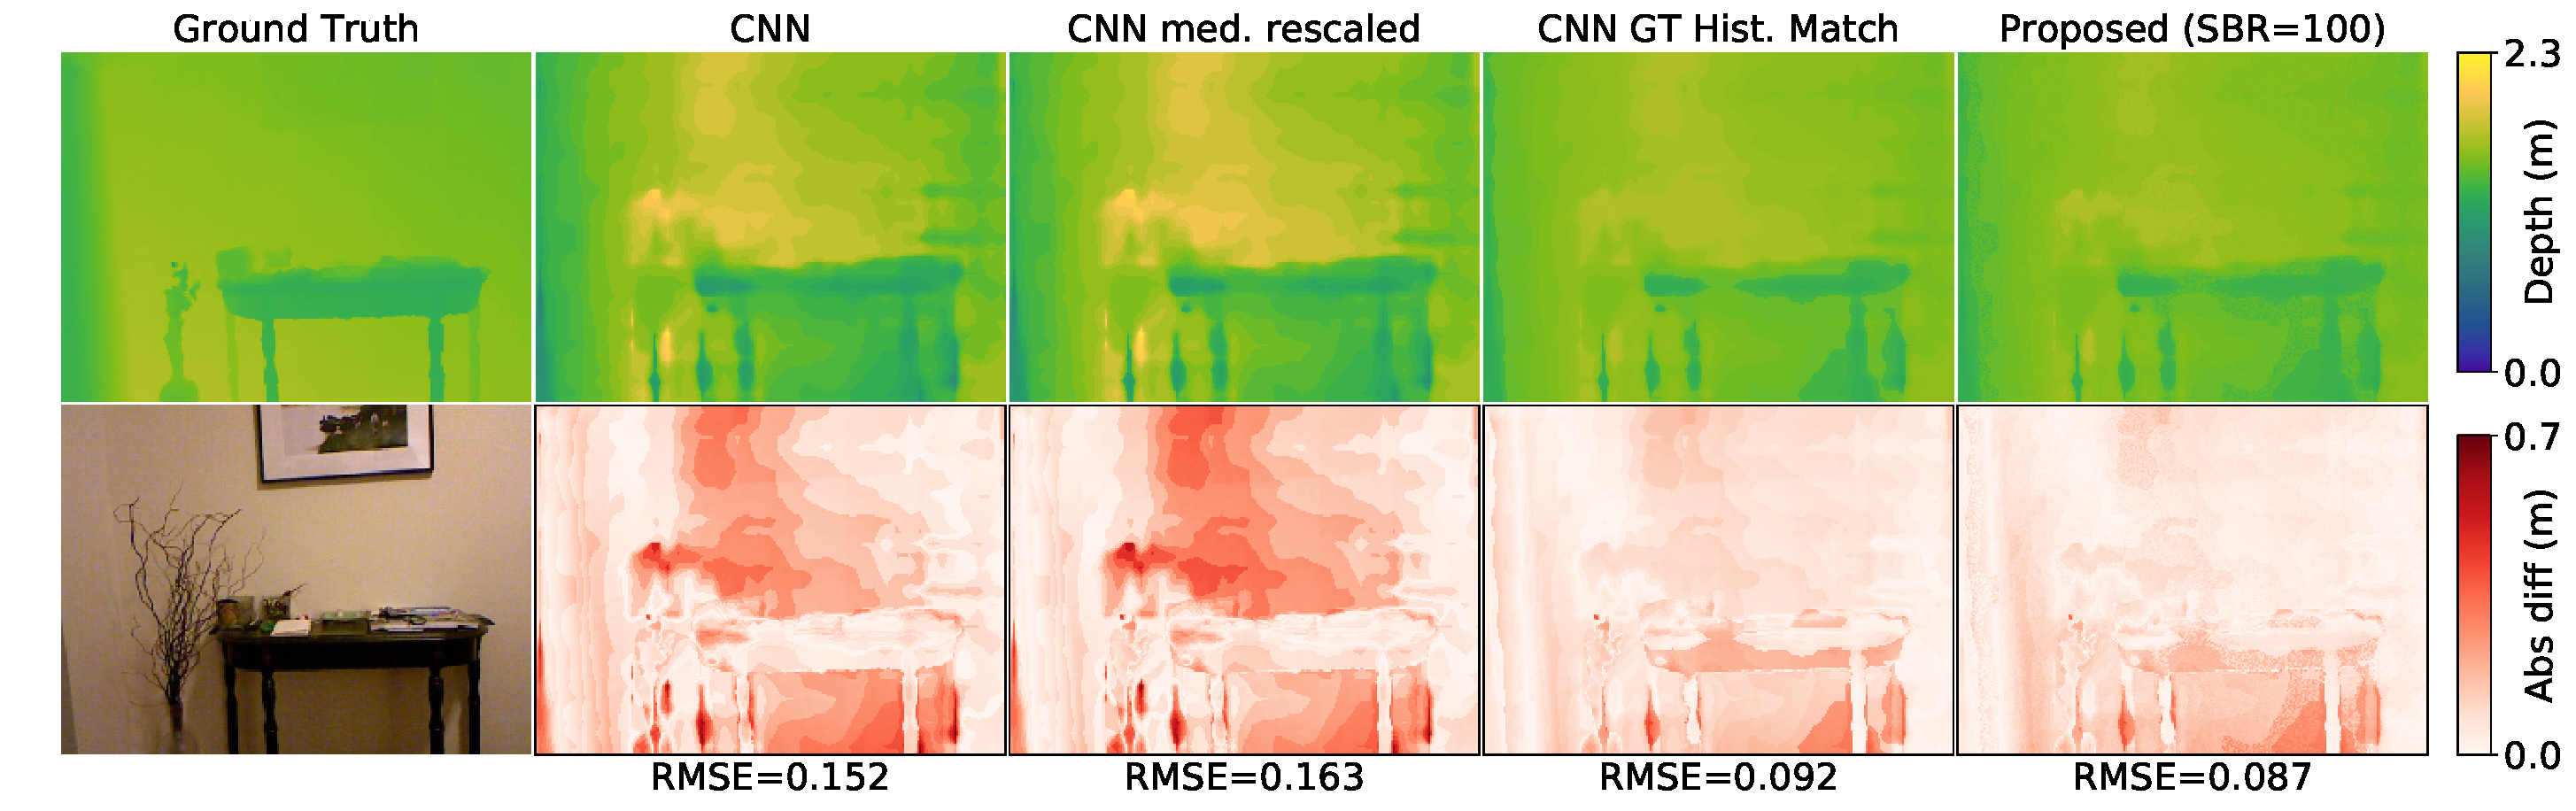
\includegraphics[width=\textwidth]{comparison/dorn_63_comparison.pdf}
  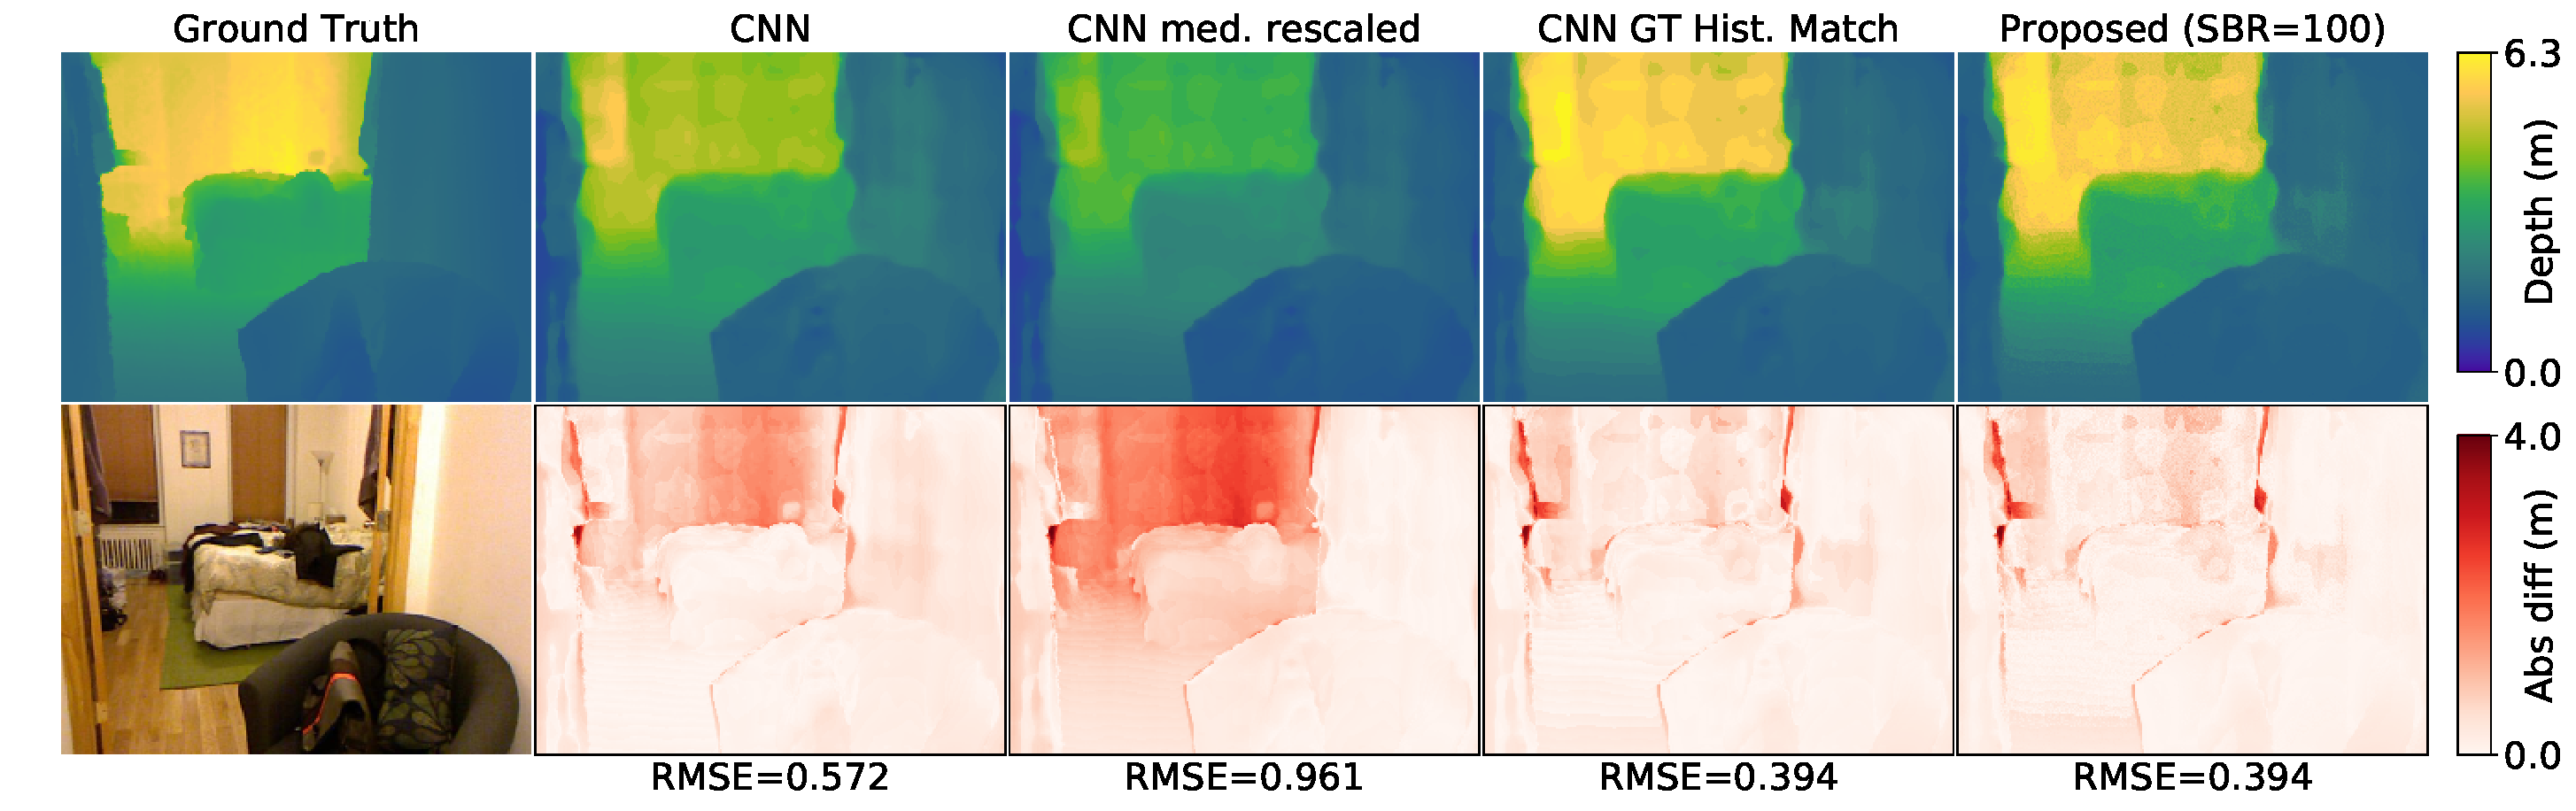
\includegraphics[width=\textwidth]{comparison/dorn_67_comparison.pdf}
  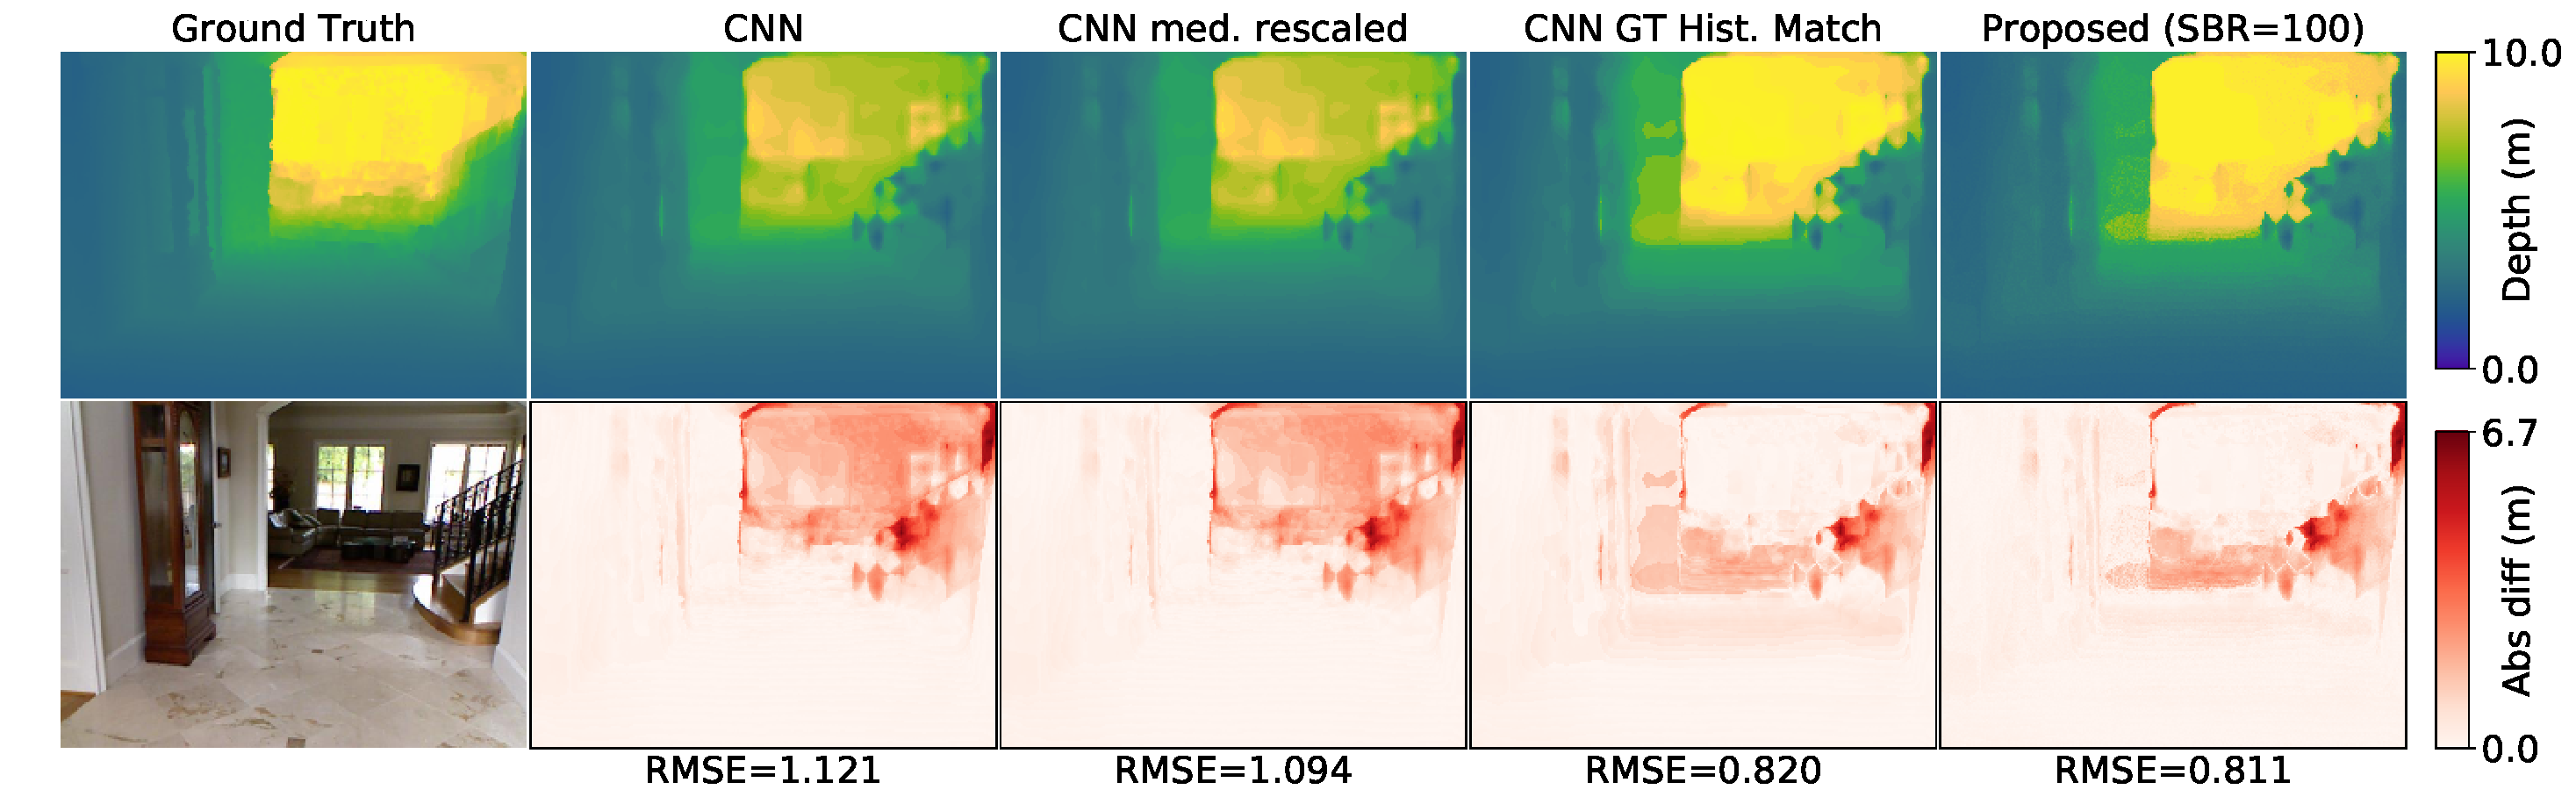
\includegraphics[width=\textwidth]{comparison/dorn_140_comparison.pdf}
  \caption{Results with DORN as the monocular depth estimator. Our method is able to scale and shift
    the depth maps to mitigate gross errors in depth scaling.}
  \label{fig:dorn_2}
\end{figure}
\begin{figure}[H]
  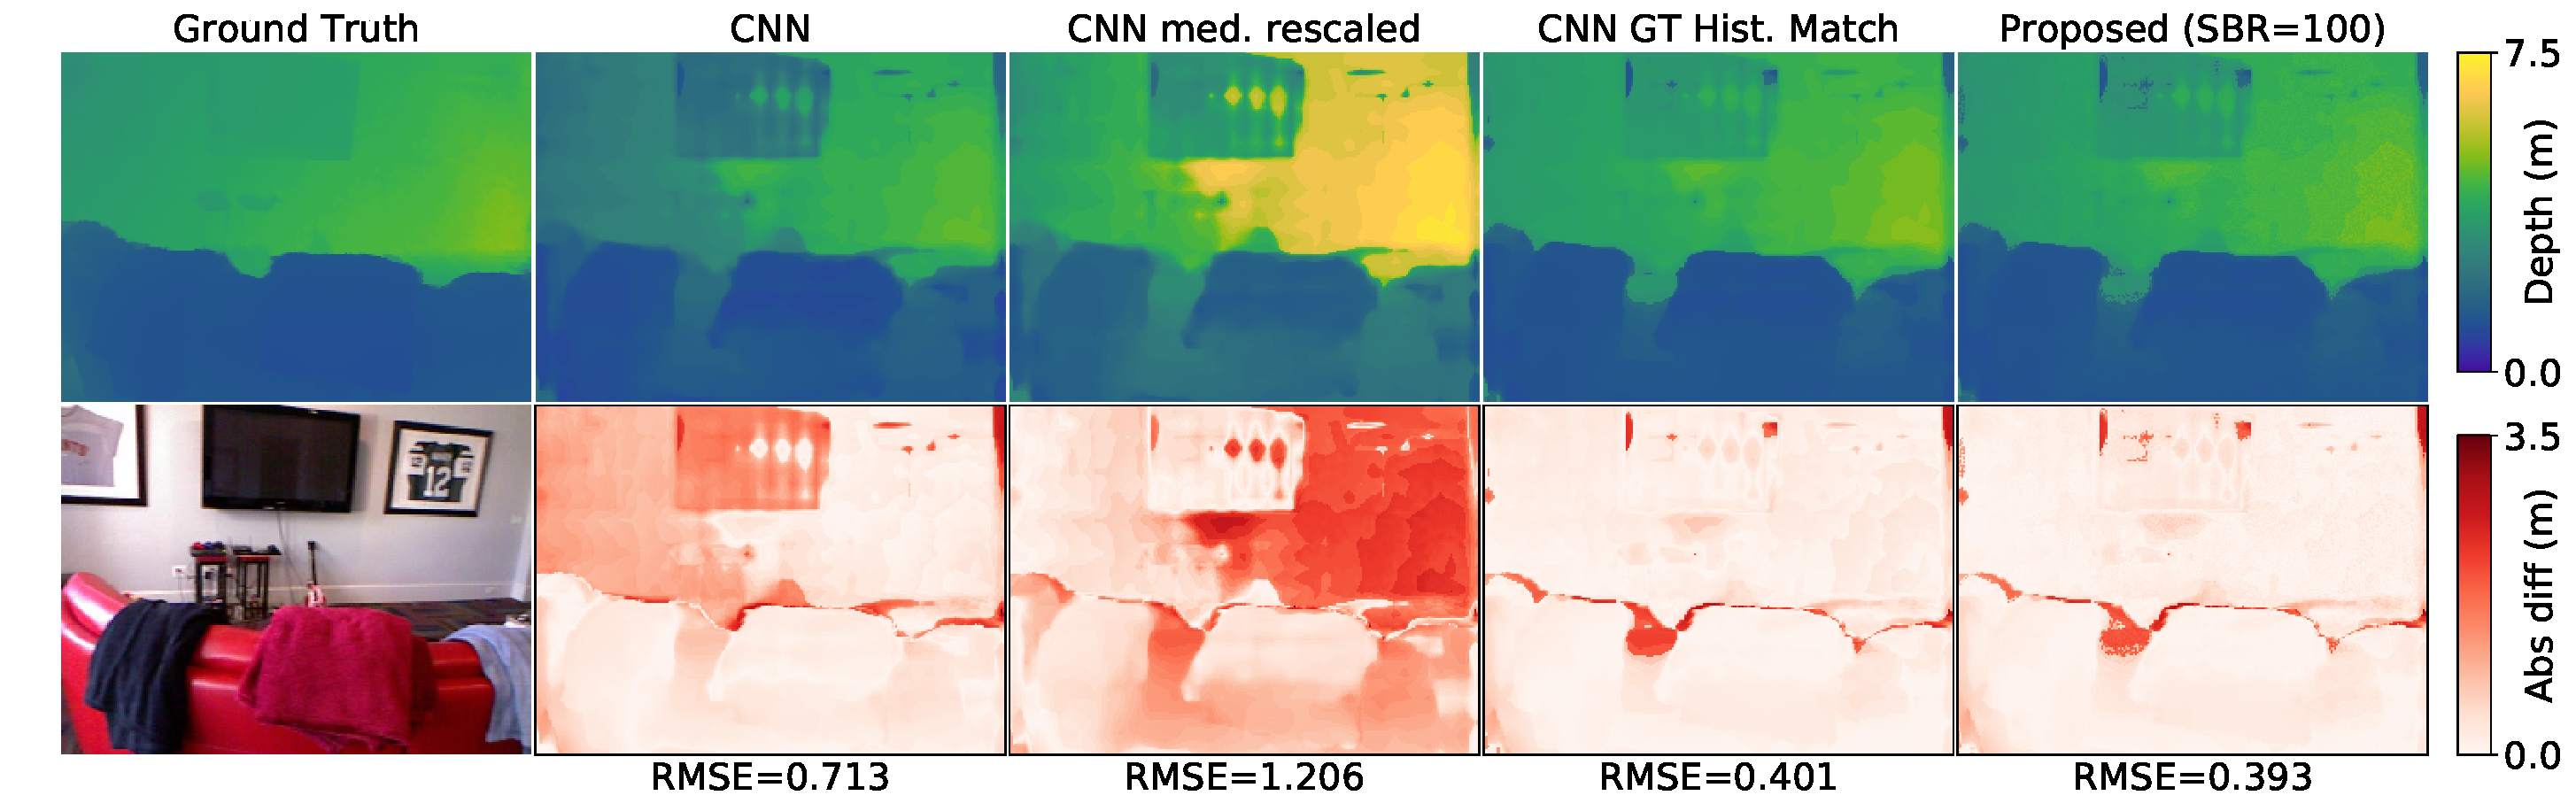
\includegraphics[width=\textwidth]{comparison/dorn_170_comparison.pdf}
  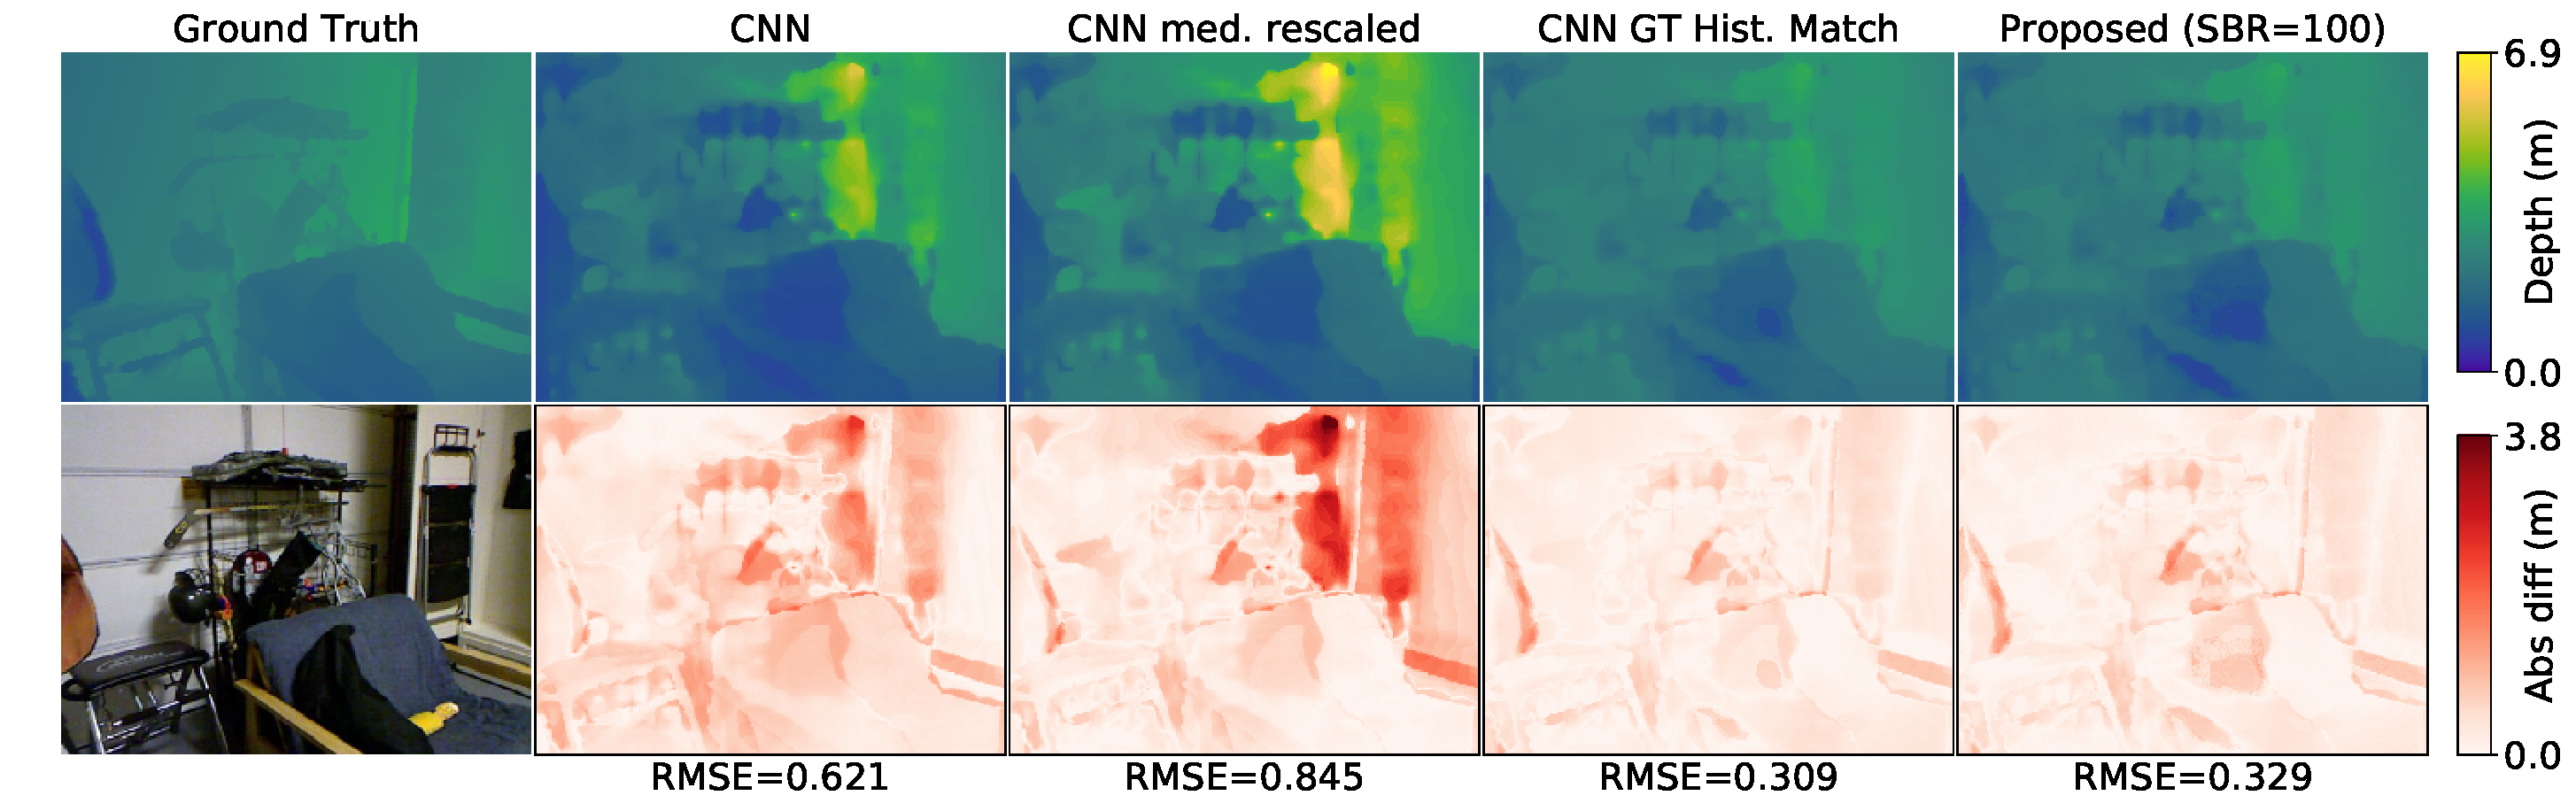
\includegraphics[width=\textwidth]{comparison/dorn_522_comparison.pdf}
  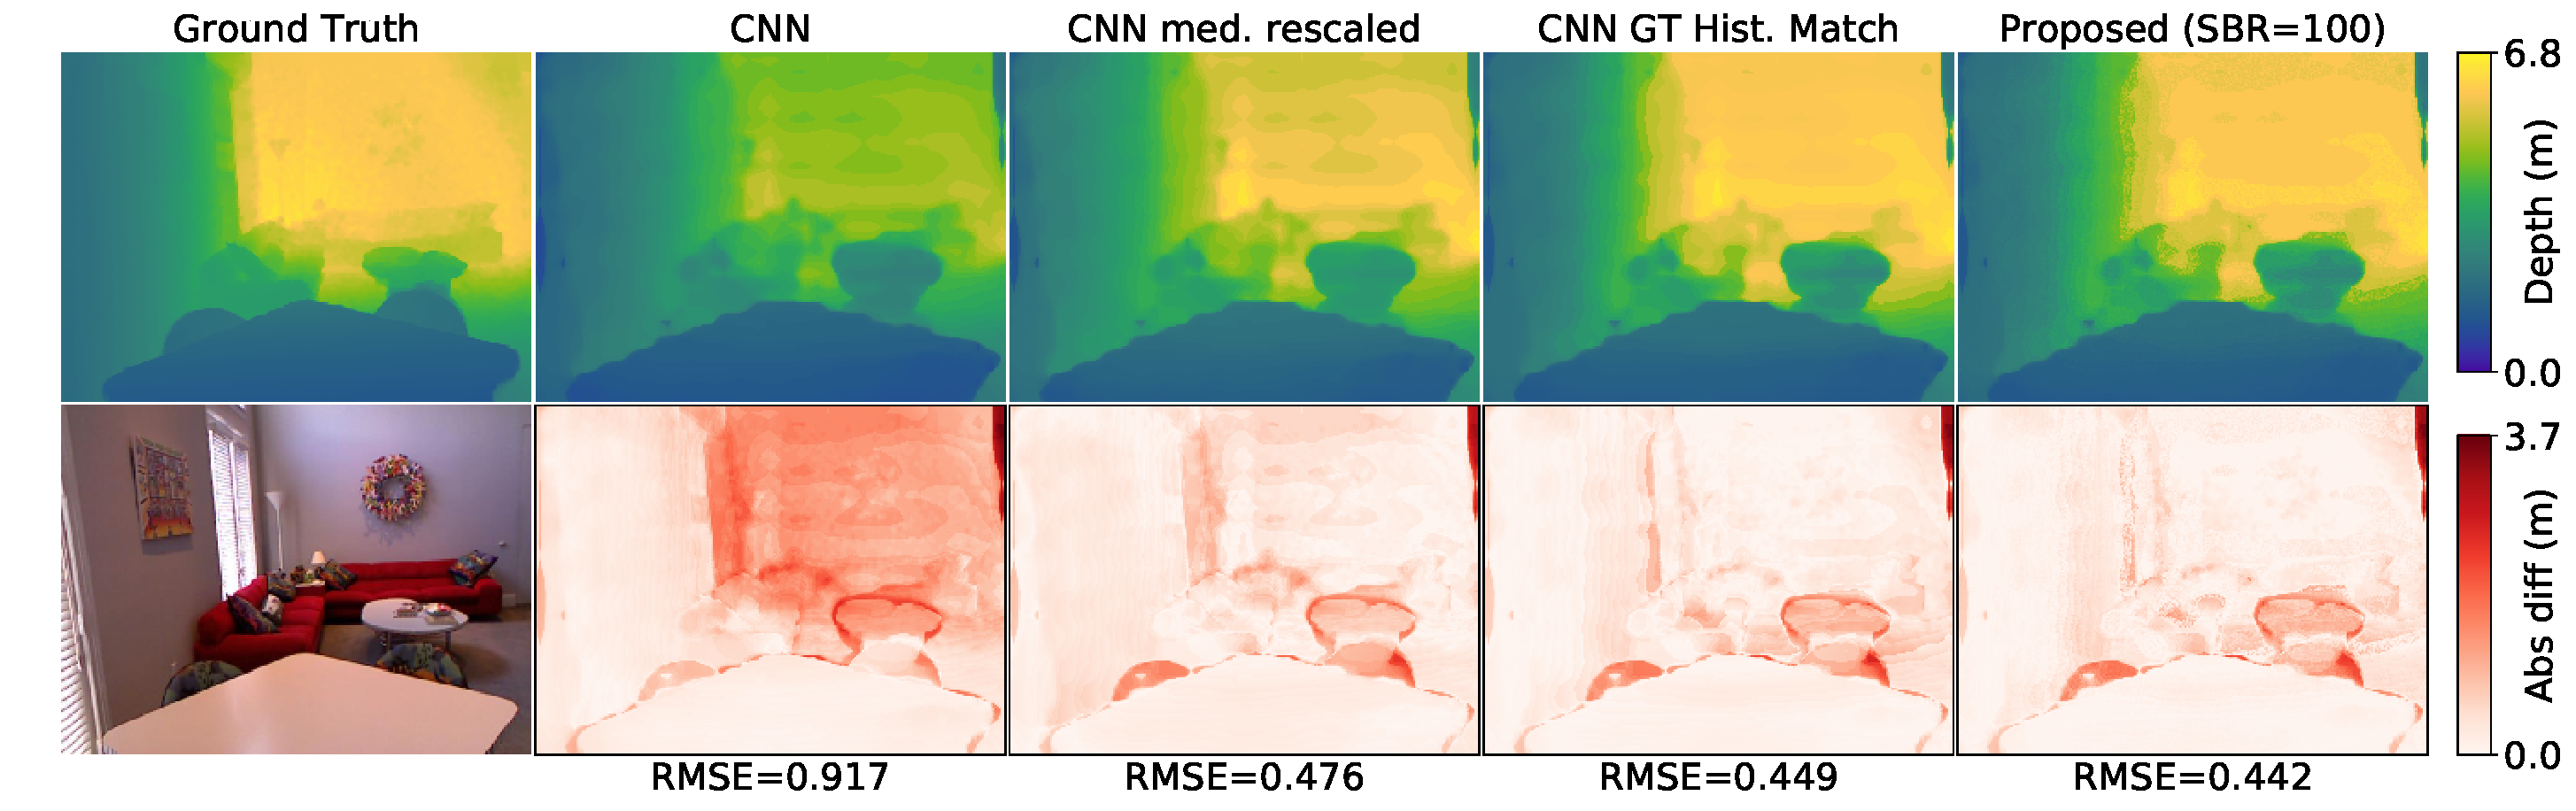
\includegraphics[width=\textwidth]{comparison/dorn_548_comparison.pdf}
  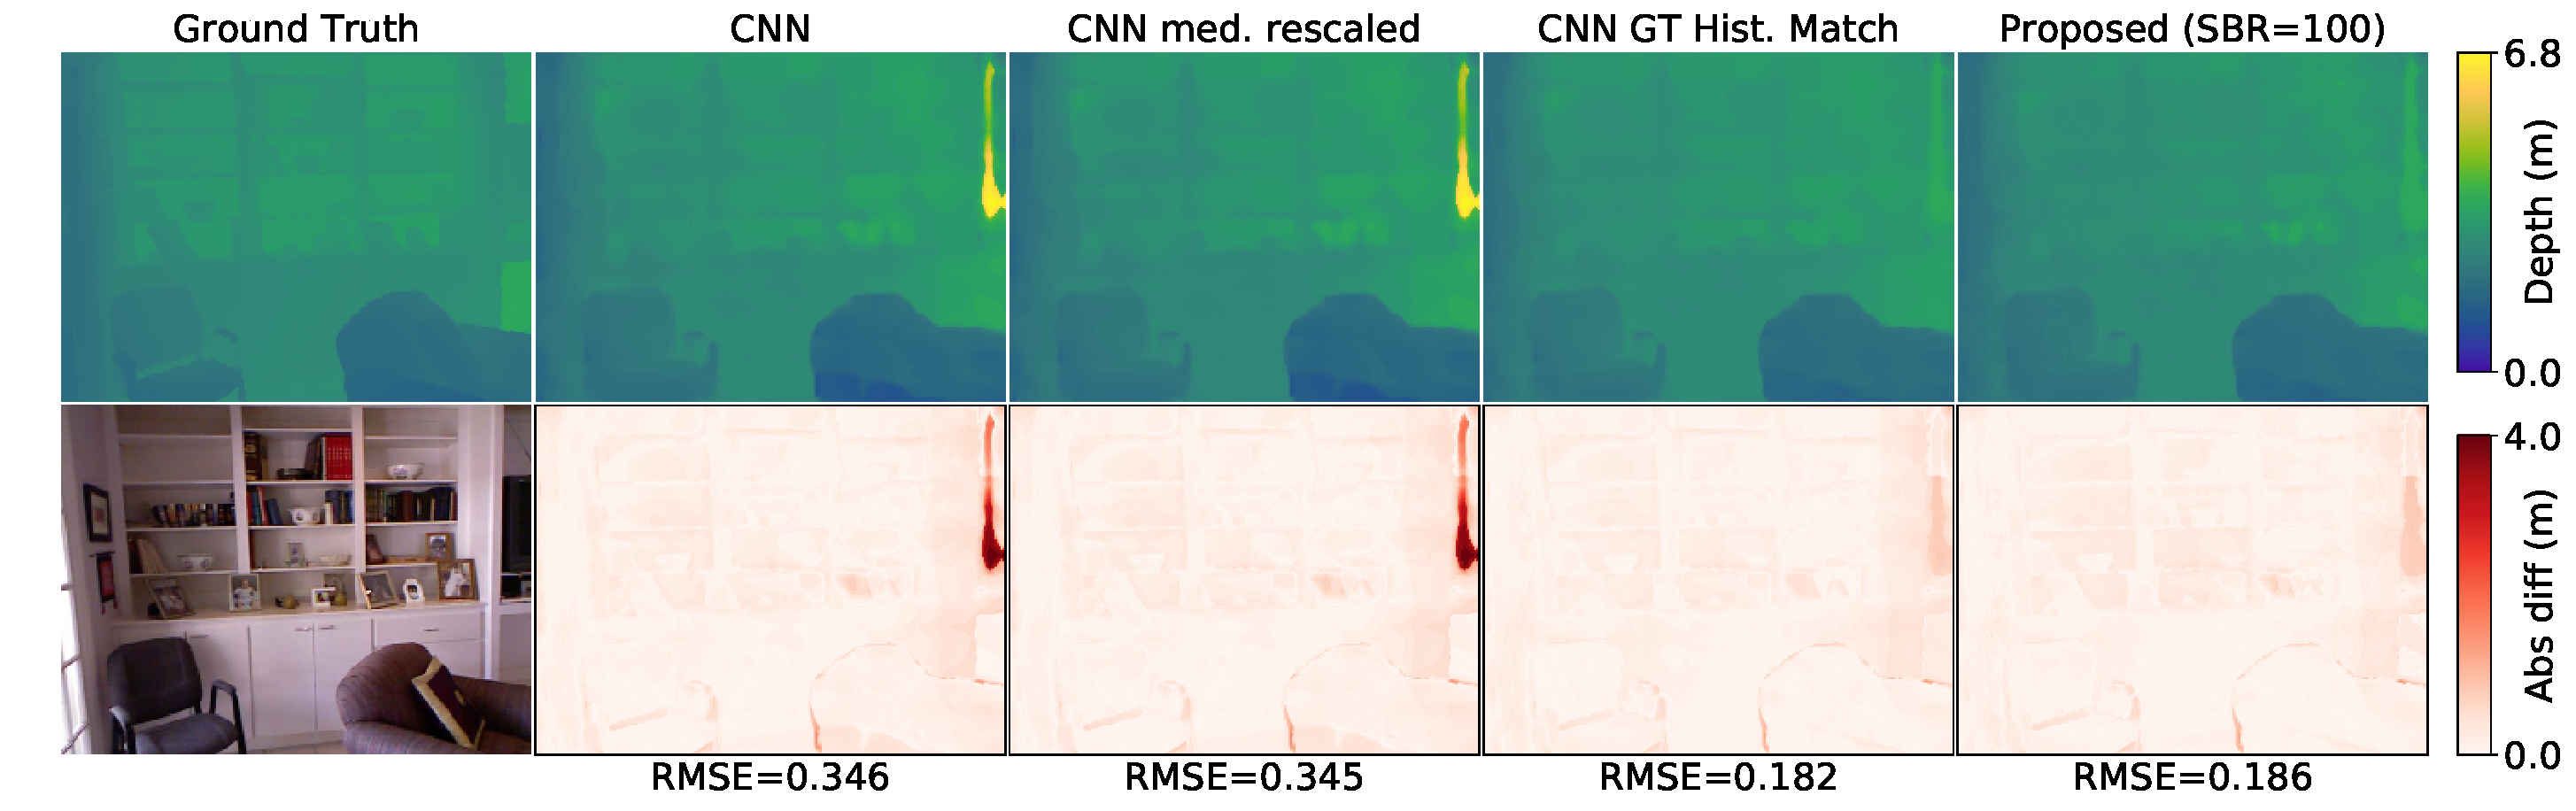
\includegraphics[width=\textwidth]{comparison/dorn_569_comparison.pdf}
  \caption{Results with DORN as the monocular depth estimator. Our method is able to scale and shift
    the depth maps to mitigate gross errors in depth scaling.}
  \label{fig:dorn_3}
\end{figure}
% \begin{figure}
%   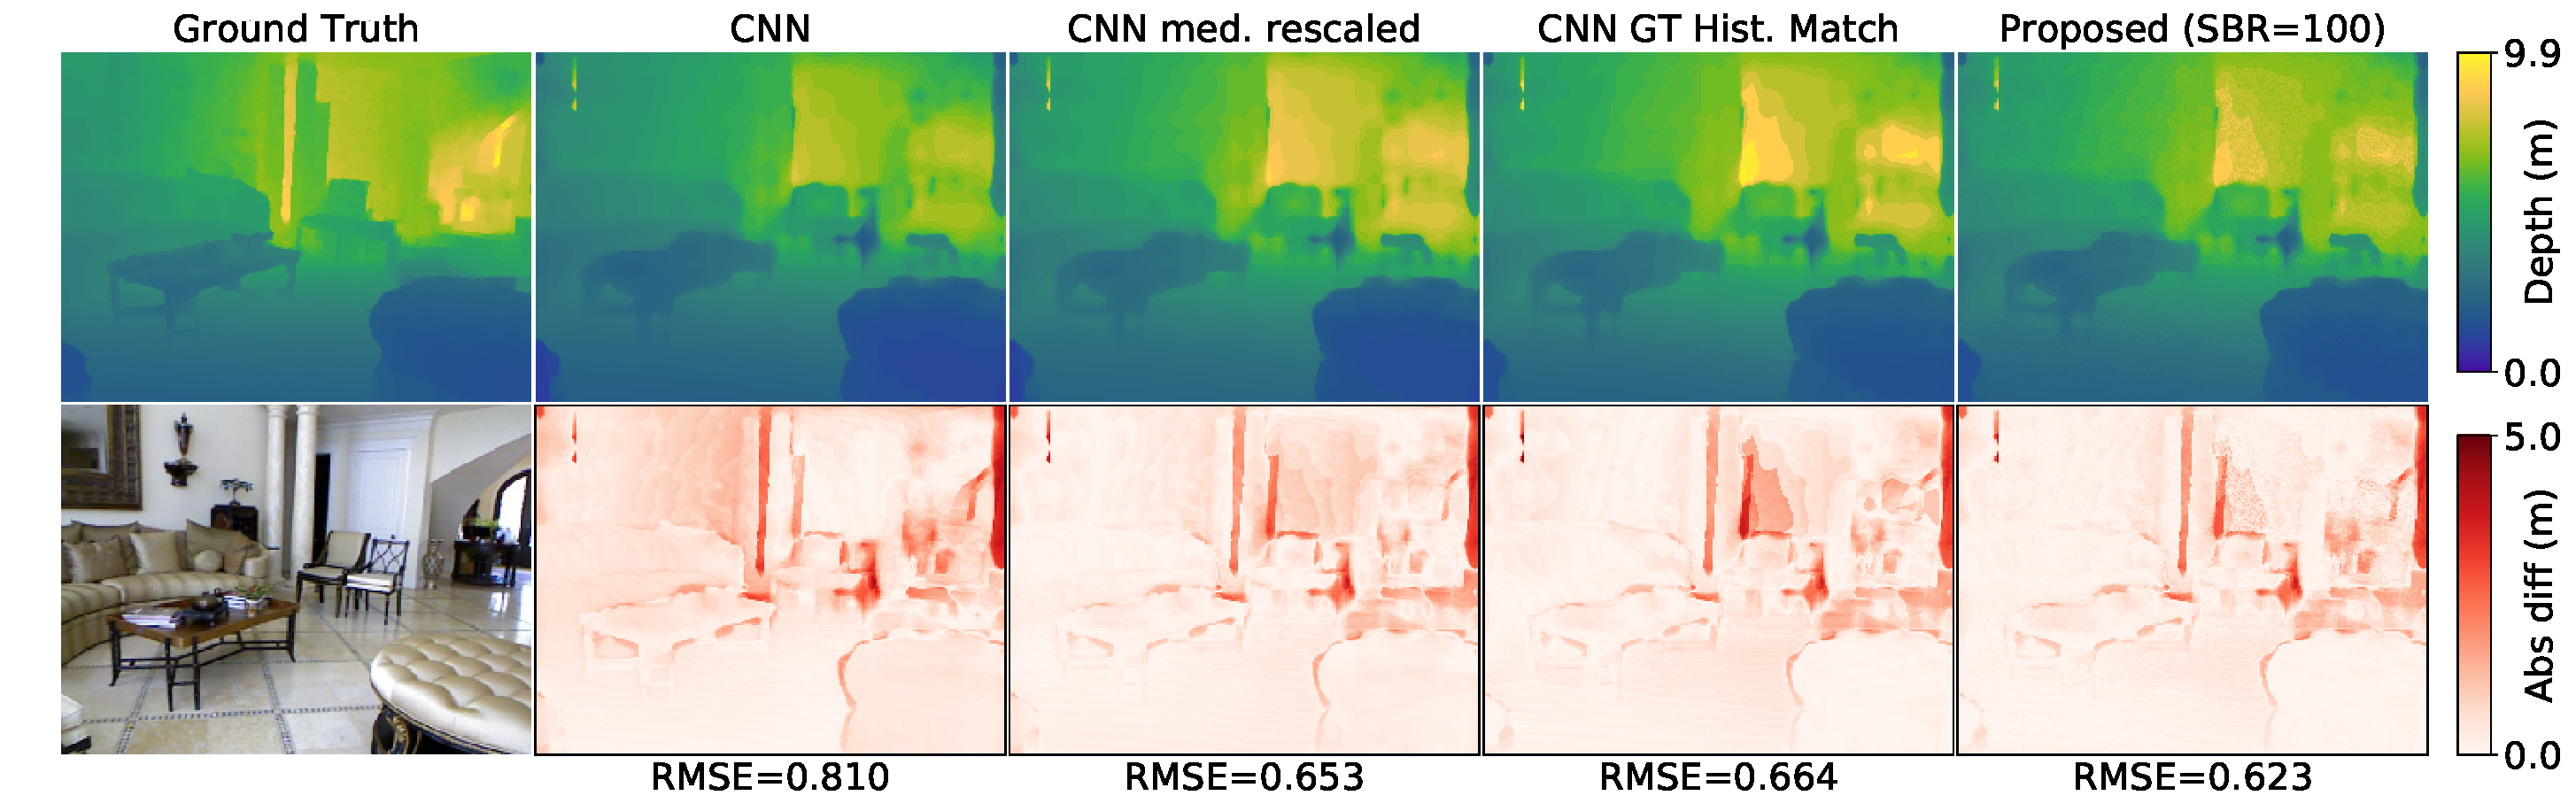
\includegraphics[width=\textwidth]{comparison/dorn_585_comparison.pdf}
%   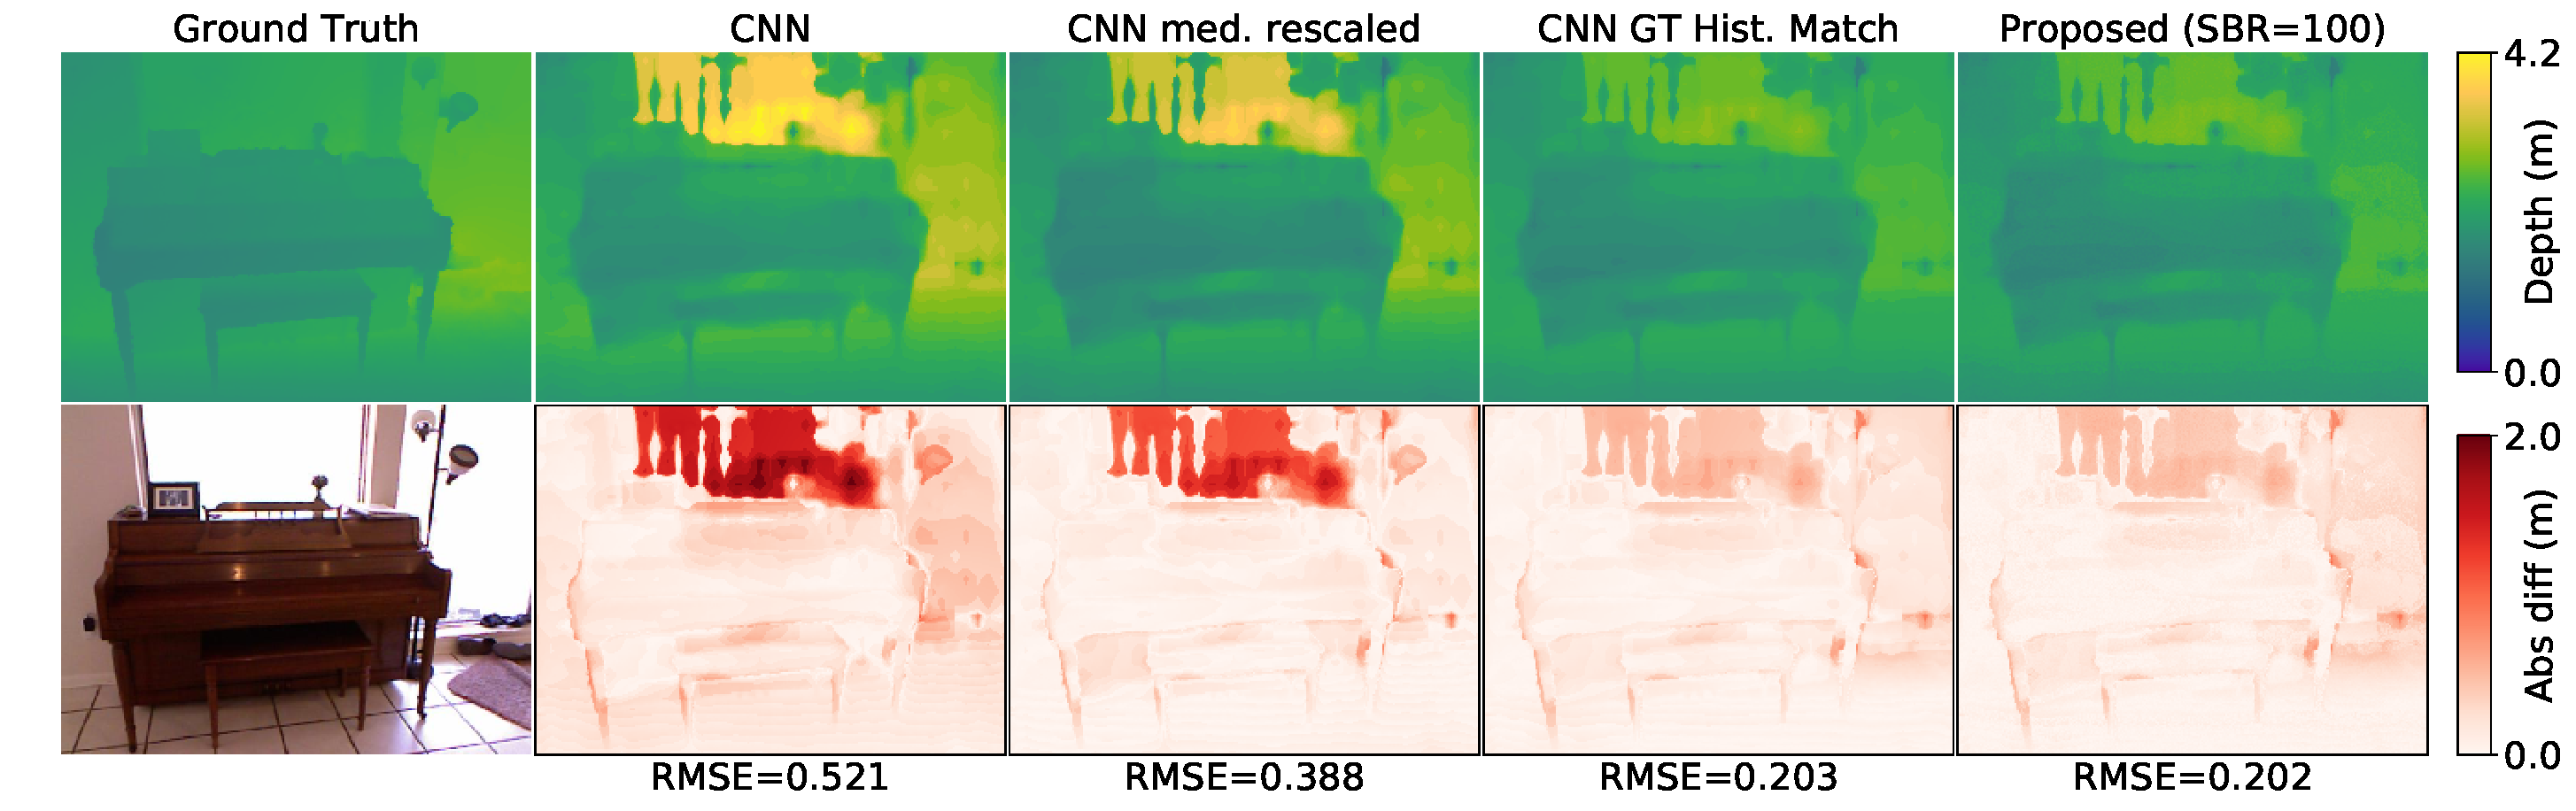
\includegraphics[width=\textwidth]{comparison/dorn_633_comparison.pdf}
%   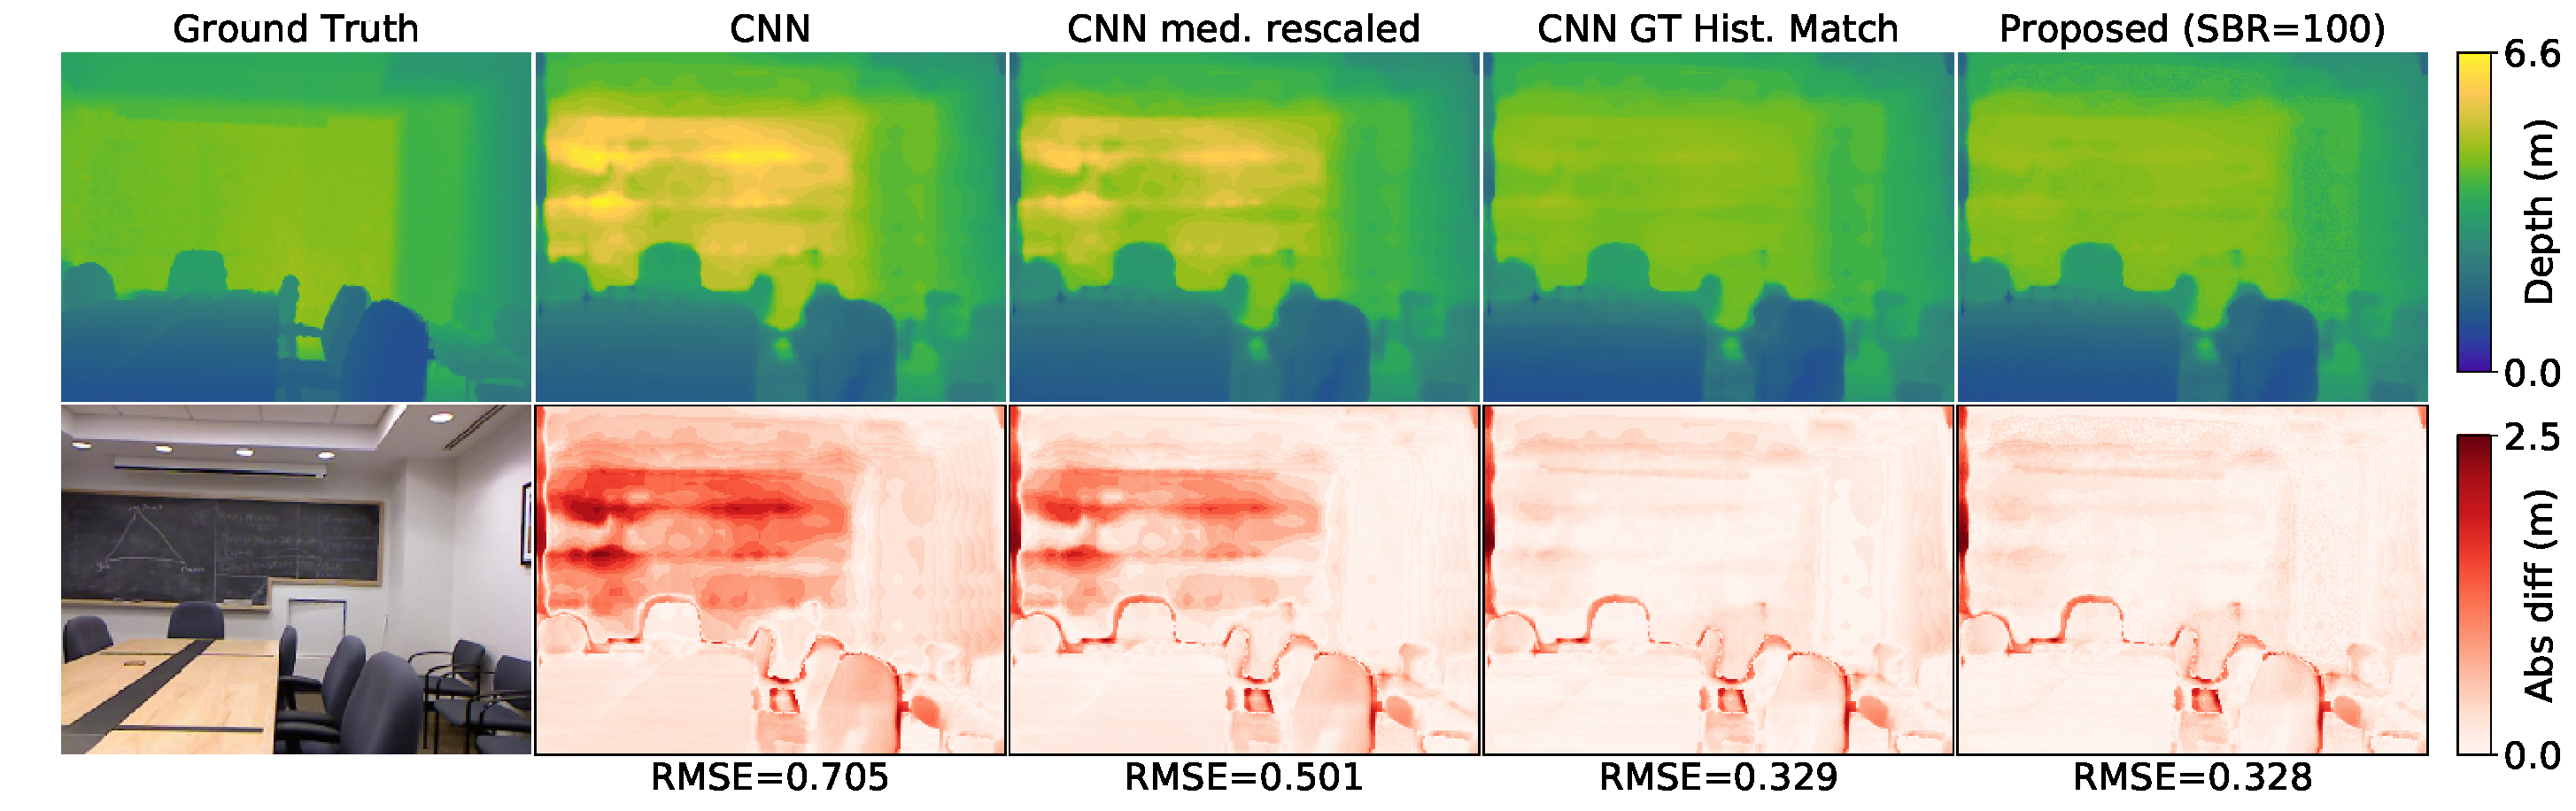
\includegraphics[width=\textwidth]{comparison/dorn_105_comparison.pdf}
%   \includegraphics[width=\textwidth]{comparison/dorn_220_comparison.pdf}
%   \caption{Results on DORN}
% \end{figure}
% \begin{figure}
%   \includegraphics[width=\textwidth]{comparison/dorn_252_comparison.pdf}
%   \includegraphics[width=\textwidth]{comparison/dorn_259_comparison.pdf}
%   \includegraphics[width=\textwidth]{comparison/dorn_178_comparison.pdf}
%   \includegraphics[width=\textwidth]{comparison/dorn_219_comparison.pdf}
%   \caption{Results on DORN}
% \end{figure}
% \begin{figure}
%   \includegraphics[width=\textwidth]{comparison/dorn_280_comparison.pdf}
%   \includegraphics[width=\textwidth]{comparison/dorn_293_comparison.pdf}
%   \includegraphics[width=\textwidth]{comparison/dorn_313_comparison.pdf}
%   \includegraphics[width=\textwidth]{comparison/dorn_413_comparison.pdf}
%   \caption{Results on DORN}
% \end{figure}
% \begin{figure}
  % \includegraphics[width=\textwidth]{comparison/dorn_477_comparison.pdf}
  % \includegraphics[width=\textwidth]{comparison/dorn_502_comparison.pdf}
%  \includegraphics[width=\textwidth]{comparison/dorn_428_comparison.pdf}
%  \includegraphics[width=\textwidth]{comparison/dorn_428_comparison.pdf}
  % \caption{Results on DORN}
% \end{figure}
% Densedepth:
% - Office: 18, 21
% - Bathroom: 25, 194, 285
% - Bookstore: 42
% - Kitchen: 52, 53, 103, 224, 226, 352, 362, 379
% - Office: 107, 187
% - Living Room: 140, 244, 527, 529
% - Dining Room: 219, 329, 346, 616
% - Bedroom: 390, 412, 420, 428, 457*, 468*, 477, 499
% Failure Cases: 258, 338(?), 341, 537 649 (minor)
% 
% DORN:
% - Office: 8, 14, 15, 23, 26
% - Living room: 63, 67, 140, 170, 522, 548, 569, 585, 633
% - Office: 105, 220, 252, 259* (interesting)
% - Kitchen: 178
% - Dining Room: 219
% - Bathroom: 280, 293, 313
% - Bedroom: 413, 477, 502
% 
% Failure Cases: 96, 266(?)
\begin{figure}[H]
  \includegraphics[width=\textwidth]{comparison/midas_597_comparison.pdf}
  \includegraphics[width=\textwidth]{comparison/midas_3_comparison.pdf}
  \includegraphics[width=\textwidth]{comparison/midas_61_comparison.pdf}
  \includegraphics[width=\textwidth]{comparison/midas_68_comparison.pdf}
  \caption{Results with MiDaS as the monocular depth estimator. Our method is able to scale and shift
    the depth maps to mitigate gross errors in depth scaling.}
  \label{fig:midas_1}
\end{figure}
\begin{figure}[H]
  \includegraphics[width=\textwidth]{comparison/midas_121_comparison.pdf}
  \includegraphics[width=\textwidth]{comparison/midas_218_comparison.pdf}
  \includegraphics[width=\textwidth]{comparison/midas_301_comparison.pdf}
  \includegraphics[width=\textwidth]{comparison/midas_337_comparison.pdf}
  \caption{Results with MiDaS as the monocular depth estimator. Our method is able to scale and shift
    the depth maps to mitigate gross errors in depth scaling.}
  \label{fig:midas_2}
\end{figure}
\begin{figure}[H]
  \includegraphics[width=\textwidth]{comparison/midas_408_comparison.pdf}
  \includegraphics[width=\textwidth]{comparison/midas_572_comparison.pdf}
  \includegraphics[width=\textwidth]{comparison/midas_15_comparison.pdf}
  \includegraphics[width=\textwidth]{comparison/midas_556_comparison.pdf}
  \caption{Results with MiDaS as the monocular depth estimator. Our method is able to scale and shift
    the depth maps to mitigate gross errors in depth scaling.}
  \label{fig:midas_3}
\end{figure}
